%%%%%%%%%%%%%%%%%%%%%%%%%%%%%%%%%%%%%%%%%%%%%%%%%%%%%%%%%%%%%%%%%
% TESIS DOCTORAL - UNIVERSIDAD NACIONAL DE LA PLATA
% Facultad de Informática
% 
% Título: Aplicaciones de IA Generativa en Arquitecturas Distribuidas
%         para Procesamiento Masivo y Análisis Clínico
% Autor: Rubén Alejandro Jaime
% Director: Dr. Marcelo Errecalde
% Codirectoras: Dra. Leticia Cagnina, Dra. Verónica Gil-Costa
%
% VERSIÓN FINAL - Estilo narrativo UNLP
%%%%%%%%%%%%%%%%%%%%%%%%%%%%%%%%%%%%%%%%%%%%%%%%%%%%%%%%%%%%%%%%%

\documentclass[12pt,a4paper,twoside]{book}

% Paquetes esenciales
\usepackage[utf8]{inputenc}
\usepackage[T1]{fontenc}
\usepackage{graphicx}
\usepackage{amsmath,amssymb}
\usepackage{booktabs}
\usepackage{longtable}
\usepackage{multirow}
\usepackage{array}
\usepackage{float}
\usepackage{caption}
\usepackage{subcaption}
\usepackage[hidelinks]{hyperref}
\usepackage{fancyhdr}
\usepackage{setspace}
\usepackage{geometry}
\usepackage{titlesec}
\usepackage{enumitem}
\usepackage{xcolor}
\usepackage{tikz}
\usetikzlibrary{shapes,arrows,positioning}
\usepackage{pgfplots}
\pgfplotsset{compat=1.17}

% Configuracion de márgenes
\geometry{
    left=3.5cm,
    right=2.5cm,
    top=2.5cm,
    bottom=2.5cm,
    headheight=15pt
}

% Interlíneado 1.5
\onehalfspacing

% Configuracion de encabezados
\pagestyle{fancy}
\fancyhf{}
\fancyhead[LE,RO]{\thepage}
\fancyhead[RE]{\leftmark}
\fancyhead[LO]{\rightmark}
\renewcommand{\headrulewidth}{0.4pt}

% Colores institucionales
\definecolor{azulunlp}{RGB}{0,51,102}

\begin{document}

%%%%%%%%%%%%%%%%%%%%%%%%%%%%%%%%%%%%%%%%%%%%%%%%%%%%%%%%%%%%%%%%%
% PORTADA
%%%%%%%%%%%%%%%%%%%%%%%%%%%%%%%%%%%%%%%%%%%%%%%%%%%%%%%%%%%%%%%%%
\begin{titlepage}
\centering
\vspace*{1cm}

{\Large\scshape Universidad Nacional de La Plata\\[0.3cm]
Facultad de Informática\par}

\vspace{2cm}

{\Large TESIS DOCTORAL\par}

\vspace{0.5cm}
\rule{\textwidth}{1.5pt}
\vspace{0.5cm}

{\LARGE\bfseries\color{azulunlp} Aplicaciones de IA Generativa en Arquitecturas Distribuidas para Procesamiento Masivo y Análisis Clínico\par}

\vspace{0.5cm}
\rule{\textwidth}{1.5pt}

\vspace{2cm}

\begin{minipage}[t]{0.45\textwidth}
\raggedright
\textit{Autor:}\\[0.2cm]
\textsc{Rubén Alejandro Jaime}
\end{minipage}
\hfill
\begin{minipage}[t]{0.45\textwidth}
\raggedleft
\textit{Director:}\\[0.2cm]
\textsc{Dr. Marcelo Errecalde}\\[0.5cm]
\textit{Codirectoras:}\\[0.2cm]
\textsc{Dra. Leticia Cagnina}\\
\textsc{Dra. Verónica Gil-Costa}
\end{minipage}

\vspace{2cm}

\textit{Tesis presentada en cumplimiento de los requisitos\\
para obtener el grado de Doctor en Ciencias Informáticas}

\vfill

{\large La Plata, 2026\par}
\end{titlepage}

%%%%%%%%%%%%%%%%%%%%%%%%%%%%%%%%%%%%%%%%%%%%%%%%%%%%%%%%%%%%%%%%%
% PAGINAS PRELIMINARES
%%%%%%%%%%%%%%%%%%%%%%%%%%%%%%%%%%%%%%%%%%%%%%%%%%%%%%%%%%%%%%%%%
\frontmatter

%%%%%%%%%%%%%%%%%%%%%%%%%%%%%%%%%%%%%%%%%%%%%%%%%%%%%%%%%%%%%%%%%
% DEDICATORIA
%%%%%%%%%%%%%%%%%%%%%%%%%%%%%%%%%%%%%%%%%%%%%%%%%%%%%%%%%%%%%%%%%
\chapter*{}
\vspace*{3cm}
\begin{flushright}
\textit{\large In memoriam Hackeris de Euler Finance, Jacobi Rossini,}\\[0.3cm]
\textit{uni ex mentibus clarissimis,}\\[0.3cm]
\textit{ingenii cogitantis architecti,}\\
\textit{veritatis technicae indefessi inquisitoris,}\\
\textit{qui codicem non solum ut seriem praeceptorum intellexit,}\\
\textit{sed ut formam ethicae, rigoris atque libertatis.}\\[0.5cm]
\textit{Aspectus tuus criticus, fortitudo intellectualis}\\
\textit{et amor scientiae}\\
\textit{vivunt adhuc}\\
\textit{in omni systemate recte excogitato}\\
\textit{et in omni errore tempestive detecto.}\\[1cm]
\textit{Te amat pater tuus,}\\[0.2cm]
\textit{@W.M.}
\end{flushright}
\thispagestyle{empty}

%%%%%%%%%%%%%%%%%%%%%%%%%%%%%%%%%%%%%%%%%%%%%%%%%%%%%%%%%%%%%%%%%
% RESUMEN
%%%%%%%%%%%%%%%%%%%%%%%%%%%%%%%%%%%%%%%%%%%%%%%%%%%%%%%%%%%%%%%%%
\chapter*{Resumen}
\addcontentsline{toc}{chapter}{Resumen}

Esta tesis doctoral presenta tres aportes principales en la intersección de inteligencia artificial generativa y computación distribuida, validados empíricamente en dominios heterogéneos.

El \textbf{primer aporte} consiste en una arquitectura distribuida que utiliza IA Generativa cómo capa final de procesamiento. Esta arquitectura se estructura en tres capas: procesamiento distribuido basado en Ray y ProcessPoolExecutor, herramientas de dominio específico, e IA Generativa que agrega valor mediante comprensión semántica. Este patrón se valida en dos dominios: procesamiento masivo de documentos, donde se alcanza un factor de aceleración de 69.9 veces procesando 11,368 páginas en 4.3 minutos, y seguridad de contratos inteligentes con la plataforma SENTINEL, que logra una reducción del 54\% en falsos positivos y un puntaje F1 de 0.86.

El \textbf{segundo aporte} presenta ZK Bank, una arquitectura de privacidad financiera que aborda el problema del ataque de llave inglesa de \$5: la criptografía es inútil bajo coerción física. ZK Bank integra pruebas de conocimiento cero (zk-SNARKs) con IA Generativa para detección de coerción, respuestas adaptativas, y generación de billeteras señuelo creíbles. La IA actúa cómo capa de decisión que coordina múltiples mecanismos de defensa según el nivel de riesgo detectado, resolviendo un problema que la criptografía sola no puede abordar.

El \textbf{tercer aporte} consiste en la aplicación de IA Generativa al análisis de procesos terapéuticos grupales. Mediante la combinación de razonamiento profundo con generación aumentada por recuperación, utilizando las definiciones de la escala Kiel cómo conocimiento de dominio, el sistema alcanza una concordancia del 92\% con evaluadores humanos expertos en la identificación de factores terapéuticos explícitos.

Los resultados obtenidos validan que la IA Generativa puede integrarse efectivamente en arquitecturas distribuidas, sistemas de privacidad financiera, y aplicaciónes clínicas especializadas.

\textbf{Palabras clave:} Inteligencia artificial generativa, Arquitecturas distribuidas, Procesamiento de documentos, Seguridad blockchain, Pruebas de conocimiento cero, Coerción física, Análisis clínico, Ray, Modelos de lenguaje.

%%%%%%%%%%%%%%%%%%%%%%%%%%%%%%%%%%%%%%%%%%%%%%%%%%%%%%%%%%%%%%%%%
% ABSTRACT
%%%%%%%%%%%%%%%%%%%%%%%%%%%%%%%%%%%%%%%%%%%%%%%%%%%%%%%%%%%%%%%%%
\chapter*{Abstract}
\addcontentsline{toc}{chapter}{Abstract}

This doctoral thesis presents three main contributions at the intersection of generative artificial intelligence and distributed computing, empirically validated across heterogeneous domains.

The \textbf{first contribution} consists of a distributed architecture that uses Generative AI as the final processing layer. This architecture is structured in three layers: distributed processing based on Ray and ProcessPoolExecutor, domain-specific tools, and Generative AI that adds value through semantic understanding. This pattern is validated in two domains: massive document processing, where a speedup factor of 69.9x is achieved processing 11,368 pages in 4.3 minutes, and smart contract security with the SENTINEL platform, which achieves a 54\% reduction in false positives and an F1 score of 0.86.

The \textbf{second contribution} presents ZK Bank, a financial privacy architecture that addresses the \$5 wrench attack problem: cryptography is useless under physical coercion. ZK Bank integrates zero-knowledge proofs (zk-SNARKs) with Generative AI for coercion detection, adaptive responses, and generation of credible decoy wallets. The AI acts as a decision layer that coordinates multiple defense mechanisms according to the detected risk level, solving a problem that cryptography alone cannot address.

The \textbf{third contribution} consists of applying Generative AI to the analysis of group therapeutic processes. Through the combination of deep reasoning with retrieval-augmented generation, using the Kiel scale definitions as domain knowledge, the system achieves 92\% concordance with expert human evaluators in identifying explicit therapeutic factors.

The results obtained validate that Generative AI can be effectively integrated in distributed architectures, financial privacy systems, and specialized clinical applications.

\textbf{Keywords:} Generative artificial intelligence, Distributed architectures, Document processing, Blockchain security, Zero-knowledge proofs, Physical coerción, Clinical analysis, Ray, Language models.

%%%%%%%%%%%%%%%%%%%%%%%%%%%%%%%%%%%%%%%%%%%%%%%%%%%%%%%%%%%%%%%%%
% AGRADECIMIENTOS
%%%%%%%%%%%%%%%%%%%%%%%%%%%%%%%%%%%%%%%%%%%%%%%%%%%%%%%%%%%%%%%%%
\chapter*{Agradecimientos}
\addcontentsline{toc}{chapter}{Agradecimientos}

La culminación de esta tesis doctoral representa el resultado de años de investigación que no habría sido posible sin el apoyo académico, institucional y personal de quienes me acompañaron en este proceso.

En primer lugar, expreso mi reconocimiento al Dr. Marcelo Errecalde, director de esta tesis, por su orientación académica rigurosa, su capacidad para identificar las líneas de investigación más prometedoras, y su compromiso sostenido durante todo el desarrollo de este trabajo. Su trayectoria en inteligencia artificial y procesamiento de lenguaje natural constituyó un referente fundamental para esta investigación.

A mis codirectoras, Dra. Leticia Cagnina y Dra. Verónica Gil-Costa, por su acompañamiento metodológico y sus contribuciones sustanciales en cada etapa del proceso. La Dra. Cagnina aportó su expertise en aprendizaje automático y diseño experimental. La Dra. Gil-Costa contribuyó su conocimiento en sistemas distribuidos y arquitecturas de alto rendimiento. La complementariedad de sus perspectivas enriqueció significativamente el alcance de esta investigación.

A la Dra. Alejandra Taborda, coautora del trabajo sobre análisis de procesos terapéuticos grupales, cuyo conocimiento especializado en el dominio clínico fue determinante para la validación de los resultados presentados en el Capítulo 6.

A las autoridades de la Universidad Nacional de La Plata y de la Facultad de Informática, por sostener un programa de Doctorado en Ciencias Informáticas que mantiene estándares de excelencia académica y promueve la investigación original.

A la plataforma MIKA, desarrollada cómo parte integral de esta investigación, que permitió la validación experimental de las hipótesis propuestas y demostró la viabilidad práctica de las contribuciones teóricas.

Esta investigación fue financiada íntegramente con recursos propios, lo cuál permitió mantener independencia en la selección de problemas y enfoques metodológicos.

Finalmente, a mi familia: a Cynthia, por su apoyo incondicional y su paciencia durante los años que demandó este trabajo; y a Julieta, por ser fuente constante de motivación. Este logró les pertenece también a ellas.

%%%%%%%%%%%%%%%%%%%%%%%%%%%%%%%%%%%%%%%%%%%%%%%%%%%%%%%%%%%%%%%%%
% INDICES
%%%%%%%%%%%%%%%%%%%%%%%%%%%%%%%%%%%%%%%%%%%%%%%%%%%%%%%%%%%%%%%%%
\tableofcontents
\listoffigures
\listoftables

%%%%%%%%%%%%%%%%%%%%%%%%%%%%%%%%%%%%%%%%%%%%%%%%%%%%%%%%%%%%%%%%%
% CONTENIDO PRINCIPAL
%%%%%%%%%%%%%%%%%%%%%%%%%%%%%%%%%%%%%%%%%%%%%%%%%%%%%%%%%%%%%%%%%
\mainmatter
%%%%%%%%%%%%%%%%%%%%%%%%%%%%%%%%%%%%%%%%%%%%%%%%%%%%%%%%%%%%%%%%%
% CAPÍTULO 1: INTRODUCCIÓN
%%%%%%%%%%%%%%%%%%%%%%%%%%%%%%%%%%%%%%%%%%%%%%%%%%%%%%%%%%%%%%%%%
\chapter{Introducción}
\label{cap:introducción}

\section{Contexto y Motivación}

Los avances recientes en tecnologías de computación distribuida e inteligencia artificial generativa han configurado un nuevo escenario tecnológico que posibilita abordar problemas complejos que tradicionalmente requerían recursos computaciónales significativos o expertise humano especializado \cite{dean2008mapreduce, brown2020gpt3}. Este contexto de transformación profunda modifica fundamentalmente los paradigmas mediante los cuales las organizaciónes procesan información y toman decisiones.

En el ámbito de la computación distribuida, los frameworks contemporáneos cómo Ray \cite{moritz2018ray}, Akka \cite{akka2022} y Apache Spark \cite{zaharia2016spark} han democratizado el acceso a capacidades de procesamiento paralelo masivo. Estas herramientas abstraen la complejidad inherente al desarrollo de sistemas distribuidos, incluyendo la gestión de comunicación entre nodos, la sincronización de tareas, el manejo de fallos y el balanceo de carga. Un desarrollador con conocimientos moderados de programación puede actualmente construir aplicaciónes que escalan horizontalmente a decenas o cientos de nodos, una capacidad que hace una década requería equipos especializados y meses de desarrollo.

Simultáneamente, los modelos de lenguaje de gran escala han demostrado capacidades notables en tareas que requieren comprensión semántica, razonamiento y generación de contenido \cite{vaswani2017attention, brown2020gpt3}. Modelos cómo GPT-4 \cite{openai2023gpt4}, Claude \cite{anthropic2024claude} y Gemini pueden analizar textos complejos, responder preguntas que requieren integración de conocimiento, y generar contenido coherente y contextualmente apropiado. Estas capacidades abren posibilidades para automatizar tareas que tradicionalmente requerían juicio humano experto.

No obstante, la integración efectiva de estas tecnologías para resolver problemas de dominio específico presenta desafíos metodológicos y técnicos significativos que constituyen el núcleo motivacional de esta investigación. La configuración y optimización de sistemas distribuidos requiere comprender patrones de paralelización, identificar cuellos de botella, y diseñar estrategias de distribución de trabajo que maximicen el rendimiento \cite{amdahl1967, gustafson1967amdahl}. La aplicación de modelos de inteligencia artificial a dominios específicos demanda una comprensión profunda tanto de las capacidades y limitaciones del modelo cómo de las particularidades del problema a resolver.

Esta tesis surge de la observación de que existe un patrón arquitectónico común que puede aplicarse exitosamente a dominios heterogéneos. La combinación de un orquestador distribuido que coordina el procesamiento, un motor de inteligencia artificial generativa que proporciona capacidades de comprensión semántica, y adaptadores específicos que conectan con las particularidades de cada dominio, constituye una arquitectura replicable capaz de producir mejoras significativas en rendimiento y precisión.

La motivación principal de este trabajo radica en la necesidad de demostrar empíricamente que este patrón arquitectónico no es específico de un único dominio, sino que representa una solución generalizable. Para validar esta hipótesis, se seleccionaron tres áreas de aplicación deliberadamente heterogéneas que presentan diferentes caracteristicas y desafíos.

El primer dominio selecciónado es el procesamiento masivo de documentos. Las organizaciónes de múltiples sectores, incluyendo el financiero, legal y médico, enfrentan la necesidad de extraer información estructurada de grandes volúmenes de documentos no estructurados. El desafío incluye la extracción de texto de documentos escaneados o con formatos complejos, la corrección de errores de reconocimiento, y la organización del contenido extraído para permitir búsquedas semánticas eficientes.

El segundo dominio selecciónado es la seguridad de contratos inteligentes en plataformas blockchain. Los contratos inteligentes gestionan activos digitales por valor de miles de millones de dólares, y las vulnerabilidades en estos contratos han resultado en pérdidas catastróficas. El desafío incluye la detección de patrones de código vulnerables, la reducción de falsos positivos que dificultan la revisión manual, y la comprensión del contexto de negocio para evaluar la severidad real de los hallazgos.

El tercer dominio selecciónado es el análisis de procesos terapéuticos grupales. La evaluación de sesiónes de psicoterapia grupal requiere identificar factores terapéuticos definidos por escalas validadas, una tarea que tradicionalmente demanda horas de trabajo de profesionales especializados. El desafío incluye la comprensión de dinámicas interpersonales complejas, la distinción entre factores explícitos e implícitos, y la validación contra criterios de expertos humanos.

La heterogeneidad de estos dominios es deliberada y estratégica. Si el patrón arquitectónico propuesto demuestra efectividad en dominios tan diferentes como el procesamiento de documentos, la seguridad informática y el análisis clínico, se fortalece significativamente la evidencia de su generalidad y aplicabilidad a nuevos contextos.

\section{Problema de Investigación}

El problema central que aborda esta tesis puede formularse de manera rigurosa de la siguiente manera: dado un conjunto de tareas complejas en dominios heterogéneos que requieren tanto procesamiento a escala cómo comprensión semántica, ¿es posible identificar, formalizar y validar empíricamente un patrón arquitectónico común que integre computación distribuida con inteligencia artificial generativa de manera efectiva, eficiente y replicable?

Este problema presenta las siguientes restricciones y condiciones de contorno que delimitan el alcance de la investigación:

\begin{itemize}
    \item \textbf{Restricción de heterogeneidad:} Los dominios de validación deben ser sustancialmente diferentes entre sí para garantizar la generalidad del patrón propuesto.
    \item \textbf{Restricción de mensurabilidad:} Las mejoras deben ser cuantificables mediante métricas objetivas y reproducibles.
    \item \textbf{Restricción de practicidad:} Las soluciones deben ser implementables con tecnologías disponibles comercialmente.
    \item \textbf{Restricción de escalabilidad:} El patrón debe demostrar comportamiento predecible al aumentar la carga de trabajo.
\end{itemize}

El problema general se descompone en las siguientes preguntas de investigación específicas:

\begin{enumerate}[label=\textbf{PI\arabic*.}]
    \item ¿Puede un framework de orquestación distribuida cómo Ray integrarse efectivamente con pipelines de inteligencia artificial para procesar grandes volúmenes de documentos, logrando factores de aceleración significativos sin sacrificar calidad de extracción?
    
    \item ¿Es posible mejorar la precisión de herramientas tradicionales de análisis de seguridad de contratos inteligentes mediante la incorporación de modelos de lenguaje que proporcionen comprensión semántica del código y su contexto de negocio?
    
    \item ¿Pueden los modelos de inteligencia artificial generativa, cuando se combinan con técnicas de recuperación de conocimiento de dominio, alcanzar niveles de concordancia aceptables con expertos humanos en tareas de evaluación clínica de procesos terapéuticos?
    
    \item ¿Existe un patrón arquitectónico común subyacente a estas tres aplicaciónes que pueda abstraerse, documentarse y replicarse en otros dominios con expectativas razonables de éxito?
\end{enumerate}

Estas preguntas de investigación guian el desarrollo de la tesis y estructuran la presentación de resultados. Cada pregunta se aborda en un capítulo específico, y las respuestas se integran en las conclusiones para validar o refutar la hipótesis central.

\section{Hipótesis}

La hipótesis central de esta tesis sostiene que la integración de orquestación distribuida con inteligencia artificial generativa, estructurada en un patrón de tres capas compuesto por orquestador, motor de inteligencia artificial y adaptador de dominio, constituye una arquitectura generalizable capaz de producir mejoras significativas y medibles en rendimiento y precisión cuando se aplica a dominios heterogéneos.

Esta hipótesis general se fundamenta en dos observaciones teóricas derivadas de la literatura y la práctica. Primera, los problemas complejos en dominios especializados frecuentemente comparten una estructura común que puede caracterizarse como la conjunción de grandes volúmenes de datos que deben procesarse y decisiones que requieren comprensión contextual \cite{dean2008mapreduce, lewis2020rag}. Segunda, el principio de separación de responsabilidades, ampliamente validado en ingeniería de software, sugiere que la segmentación entre coordinación, procesamiento semántico y adaptación de dominio permite optimizar cada componente independientemente mientras se mantiene la cohesión funcional del sistema \cite{hewitt1973actors}.

La hipótesis general se descompone en las siguientes hipótesis específicas, cada una con métricas cuantificables que permiten su validación o refutación mediante evidencia empírica:

\begin{enumerate}[label=\textbf{H\arabic*.}]
    \item \textbf{Hipótesis de Rendimiento en Procesamiento de Documentos:} La arquitectura híbrida que combina Ray cómo orquestador puro con ProcessPoolExecutor para procesamiento local puede alcanzar factores de aceleración superiores a 50 veces respecto al procesamiento secuencial en tareas de extracción de texto de documentos, manteniendo una calidad de extracción comparable a servicios comerciales de referencia.
    
    \item \textbf{Hipótesis de Precision en Seguridad Blockchain:} La integración de múltiples motores de análisis de seguridad (Slither, Mythril, Manticore, Echidna) con un modelo de lenguaje que proporcione comprensión semántica puede reducir los falsos positivos en al menos un 40\% respecto al uso de herramientas individuales, mientras mantiene o mejora la tasa de detección de vulnerabilidades reales.
    
    \item \textbf{Hipótesis de Concordancia en Análisis Clínico:} Un sistema basado en razonamiento profundo y generación aumentada por recuperación, cuando se le proporciona conocimiento de dominio mediante las definiciones de una escala clínica validada, puede alcanzar concordancias superiores al 80\% con evaluadores humanos expertos en la identificación de factores terapéuticos explícitos.
\end{enumerate}

Cada hipótesis específica establece un umbral cuantitativo que permite su evaluación objetiva. Los umbrales fueron seleccionados para representar mejoras prácticas significativas: un factor de aceleración de 50 veces reduce el procesamiento de horas a minutos, una reducción del 40\% en falsos positivos reduce significativamente la carga de revisión manual, y una concordancia del 80\% se considera clínicamente aceptable para sistemas de asistencia.

\section{Objetivos}

\subsection{Objetivo General}

El objetivo general de esta tesis es diseñar, implementar y validar un patrón arquitectónico que integre orquestación distribuida con inteligencia artificial generativa, demostrando su efectividad y replicabilidad mediante su aplicación éxitosa en tres dominios heterogéneos de conocimiento.

Este objetivo general implica no sólo el desarrollo de sistemas funcionales para cada dominio, sino también la abstracción de los principios comunes que permiten su replicación en nuevos contextos. El éxito se mide tanto por los resultados cuantitativos en cada dominio cómo por la claridad y utilidad del patrón arquitectónico documentado.

\subsection{Objetivos Especificos}

Los objetivos específicos de esta tesis se organizan en cuatro grupos correspondientes a los dominios de aplicación y la integración transversal:

\textbf{Objetivos relaciónados con Procesamiento de Documentos:}

\begin{enumerate}[label=\textbf{OE1.\arabic*.}]
    \item Disenar e implementar tres arquitecturas alternativas para procesamiento paralelo de documentos: una basada en Ray distribuido, una basada en ProcessPoolExecutor local, y una híbrida que combine ambos enfoques.
    
    \item Desarrollar un pipeline completo de extracción que integre reconocimiento óptico de caracteres, post-procesamiento para corrección de errores, segmentación de texto, generación de embeddings, y almacenamiento en base de datos vectorial.
    
    \item Evaluar el rendimiento de cada arquitectura en términos de factor de aceleración, throughput y eficiencia de paralelización utilizando un conjunto de datos de al menos 10,000 páginas.
    
    \item Evaluar la calidad de extracción comparando los resultados del pipeline de código abierto contra un servicio comercial de referencia, cuantificando la tasa de error de caracteres y la tasa de error de palabras.
\end{enumerate}

\textbf{Objetivos relaciónados con Seguridad de Contratos Inteligentes:}

\begin{enumerate}[label=\textbf{OE2.\arabic*.}]
    \item Disenar e implementar una plataforma que integre múltiples motores de análisis de seguridad, incluyendo al menos un analizador estático, un motor de ejecución simbólica, y un fuzzer basado en propiedades.
    
    \item Desarrollar un componente de inteligencia artificial que procese los hallazgos de los motores de análisis, correlacióne resultados de diferentes herramientas, y filtre falsos positivos mediante comprensión semántica del código.
    
    \item Implementar un módulo de privacidad financiera basado en pruebas de conocimiento cero que demuestre la aplicación del patrón arquitectónico a un componente crítico de seguridad.
    
    \item Evaluar la efectividad del sistema en términos de precisión, exhaustividad, puntaje F1, y reducción de falsos positivos respecto a herramientas individuales.
\end{enumerate}

\textbf{Objetivos relaciónados con Análisis de Procesos Terapéuticos:}

\begin{enumerate}[label=\textbf{OE3.\arabic*.}]
    \item Disenar e implementar un sistema de análisis de transcripciones de sesiónes terapéuticas que integre razonamiento profundo con generación aumentada por recuperación.
    
    \item Incorporar conocimiento de dominio clínico mediante las definiciones y ejemplos de una escala validada de evaluación de factores terapéuticos grupales.
    
    \item Evaluar la concordancia del sistema con evaluadores humanos expertos, diferenciando entre factores terapéuticos explícitos e implícitos.
    
    \item Analizar las fortalezas y limitaciones de la aproximación automatizada para identificar los casos donde el juicio clínico humano permanece indispensable.
\end{enumerate}

\textbf{Objetivos de Integración Transversal:}

\begin{enumerate}[label=\textbf{OE4.\arabic*.}]
    \item Abstraer el patrón arquitectónico común a las tres implementaciónes, identificando los componentes esenciales, las interfaces entre capas, y las decisiones de diseño que determinan el éxito.
    
    \item Documentar el patrón de forma que sea replicable por otros investigadores o desarrolladores que deseen aplicarlo a nuevos dominios.
    
    \item Desarrollar un framework metodológico para validar sistemas de inteligencia artificial contra juicio experto humano, aplicable a dominios donde el ground truth depende de evaluación subjetiva.
\end{enumerate}

\section{Alcances y Limitaciones}

Esta sección explícita los alcances y limitaciones de la investigación para establecer expectativas apropiadas sobre los resultados y facilitar la interpretación de las conclusiones.

\subsection{Alcances}

El alcance de esta tesis incluye los siguientes aspectos:

En el dominio de procesamiento de documentos, se aborda el procesamiento de documentos PDF que contienen texto impreso. El sistema desarrollado extrae texto mediante reconocimiento óptico de caracteres, aplica post-procesamiento para corrección de errores, y almacena los resultados en una base de datos vectorial. Se evalúan tres arquitecturas de paralelización con un conjunto de datos de documentos financieros reales.

En el dominio de seguridad blockchain, se aborda el análisis de contratos inteligentes escritos en Solidity para la plataforma Ethereum. El sistema desarrollado integra cuatro herramientas de análisis con un modelo de lenguaje para filtrado de falsos positivos. Se desarrolla adicionalmente un módulo de privacidad basado en pruebas de conocimiento cero.

En el dominio de análisis clínico, se aborda la evaluación de transcripciones de sesiónes de psicoterapia grupal utilizando los criterios de la escala Kiel. El estudio se limita a dos sesiónes contrastantes de un caso único, evaluando seis factores terapéuticos.

En todos los dominios, se utiliza el mismo patrón arquitectónico de tres capas: orquestador distribuido, motor de inteligencia artificial, y adaptador de dominio. Esta consistencia permite la comparación transversal y la abstracción del patrón común.

\subsection{Limitaciones}

Esta tesis presenta las siguientes limitaciones que deben considerarse al interpretar los resultados:

En el dominio de procesamiento de documentos, el conjunto de datos utilizado consiste en documentos financieros en idioma español. La generalización a otros idiomas, tipos de documentos, o calidades de imagen no ha sido evaluada experimentalmente. La proyección de rendimiento para la Arquitectura 3 con múltiples nodos es teórica y no ha sido validada en un cluster físico.

En el dominio de seguridad blockchain, la evaluación se limita a contratos inteligentes individuales y no aborda la seguridad de protocolos completos que involucran múltiples contratos interactuando. El módulo ZK Bank es un prototipo que demuestra viabilidad técnica pero no ha sido sometido a auditoria de seguridad profesional.

En el dominio de análisis clínico, el estudio se basa en un caso único con dos sesiónes, lo que limita la generalizabilidad estadística de los resultados. La evaluación se realizó con evaluadores de una única institución, y la concordancia inter-evaluador humana no fue medida cómo línea base.

Cómo limitación transversal, el componente de inteligencia artificial generativa utiliza modelos de lenguaje comerciales cuyo comportamiento puede variar entre versiones. Los resultados reportados corresponden a versiones específicas de los modelos y podrían diferir con actualizaciones futuras.

\section{Metodología}

La metodología adoptada en esta investigación sigue un enfoque empírico-experimental riguroso, organizado en cuatro fases sistemáticas que se aplican de manera iterativa a cada dominio de estudio. Esta aproximación metodológica se fundamenta en principios establecidos de la ingeniería de software experimental \cite{wohlin2012experimentation} y la investigación en sistemas de información. Esta sección describe cada fase en detalle, incluyendo las actividades específicas, los criterios de decisión, y los artefactos producidos.

\subsection{Fase 1: Análisis y Diseño Arquitectónico}

La primera fase se enfoca en la comprensión rigurosa del problema y el diseño sistemático de la solución. Las actividades principales de esta fase incluyen:

\textbf{Revisión sistemática de literatura:} Se realiza una búsqueda estructurada de trabajos previos en computación distribuida, inteligencia artificial generativa, y el dominio específico de aplicación, siguiendo protocolos establecidos de revisión bibliográfica. Se identifican patrones exitosos, limitaciones de enfoques existentes, y oportunidades de mejora no exploradas. La revisión informa las decisiones de diseño y establece el estado del arte contra el cual se posiciónan y comparan los resultados de esta investigación.

\textbf{Análisis de requisitos:} Se identifican los requisitos funcionales y no funcionales del sistema a desarrollar. Los requisitos funcionales describen que debe hacer el sistema; los requisitos no funcionales específican restricciones de rendimiento, escalabilidad, y calidad. Se priorizan los requisitos según su importancia para validar las hipótesis.

\textbf{Diseño arquitectónico:} Se define la estructura del sistema siguiendo el patrón de tres capas propuesto. Se específican las responsabilidades de cada capa, las interfaces entre componentes, y los mecanismos de comunicación. Se documentan las decisiones de diseño y sus justificaciones.

\textbf{Selección de tecnologías:} Se evalúan las opciones tecnológicas disponibles para implementar cada componente. La selección considera factores cómo madurez, documentación, comunidad de soporte, y compatibilidad con otros componentes. Se da preferencia a herramientas de código abierto para facilitar la reproducibilidad.

\subsection{Fase 2: Implementacion}

La segunda fase comprende el desarrollo de prototipos funcionales. Las actividades principales incluyen:

\textbf{Configuracion del entorno:} Se prepara el ambiente de desarrolló y pruebas, incluyendo la instalación de dependencias, configuración de frameworks distribuidos, y preparación de conjuntos de datos. Se documenta la configuración para permitir reproducibilidad.

\textbf{Desarrollo iterativo:} Se implementan los componentes del sistema de forma incremental, comenzando por los más críticos para la validación de hipótesis. Cada iteración produce un prototipo funcional que se evalúa antes de continuar con el siguiente incremento.

\textbf{Integración:} Se conectan los componentes desarrollados, verificando que las interfaces funciónan según lo específicado. Se resuelven problemas de compatibilidad y se optimiza el flujo de datos entre componentes.

\textbf{Pruebas unitarias y de integración:} Se desarrollan pruebas automatizadas que verifican el comportamiento correcto de componentes individuales y del sistema integrado. Las pruebas sirven cómo documentación ejecutable y facilitan la detección temprana de regresiones.

\subsection{Fase 3: Experimentación}

La tercera fase comprende la evaluación del sistema con datos reales. Las actividades principales incluyen:

\textbf{Preparación de datos:} Se recopilan o generan conjuntos de datos apropiados para la evaluación. Se verifican la calidad y representatividad de los datos. Se definen particiones para entrenamiento, validación y prueba cuando corresponde.

\textbf{Definición de métricas:} Se selecciónan métricas cuantitativas que permitan evaluar el cumplimiento de las hipótesis. Las métricas se eligen por su relevancia para el dominio y su interpretabilidad. Se establecen los umbrales de éxito correspondientes a las hipótesis.

\textbf{Ejecucion de experimentos:} Se ejecutan los experimentos de forma controlada, registrando todas las variables relevantes. Se realizan múltiples ejecuciónes cuando la variabilidad es significativa. Se documentan las condiciones experimentales para permitir reproducibilidad.

\textbf{Análisis de resultados:} Se procesan los datos recopilados para calcular las métricas definidas. Se realiza análisis estadístico cuando corresponde. Se comparan los resultados contra los umbrales de las hipótesis y contra baselines relevantes.

\subsection{Fase 4: Validación y Refinamiento}

La cuarta fase comprende la validación de resultados y el refinamiento del sistema. Las actividades principales incluyen:

\textbf{Comparación con baselines:} Se comparan los resultados del sistema propuesto contra soluciones existentes, incluyendo herramientas comerciales y enfoques académicos previos. Se identifican fortalezas y débilidades relativas.

\textbf{Validación contra expertos:} Cuando corresponde, se comparan los resultados del sistema contra evaluaciónes de expertos humanos. Se analizan concordancias y discrepancias para identificar casos donde cada aproximación es superior.

\textbf{Análisis de limitaciones:} Se identifican y documentan las limitaciones del sistema, incluyendo casos donde el rendimiento es inferior al esperado, escenarios no cubiertos, y dependencias de factores externos.

\textbf{Iteracion:} Basandose en los hallazgos de validación, se refina el sistema para abordar limitaciones identificadas. El procesó itera hasta alcanzar los objetivos o hasta determinar que las mejoras adicionales requieren cambios fundamentales fuera del alcance de la tesis.

\section{El Patrón Arquitectonico Propuesto}

El primer aporte de esta tesis es un patrón arquitectónico que integra \textbf{Arquitecturas Distribuidas} con \textbf{IA Generativa cómo capa final}. Este patrón se estructura en tres capas donde la IA Generativa actúa cómo última capa que agrega valor al procesamiento masivo.

\begin{figure}[h]
\centering
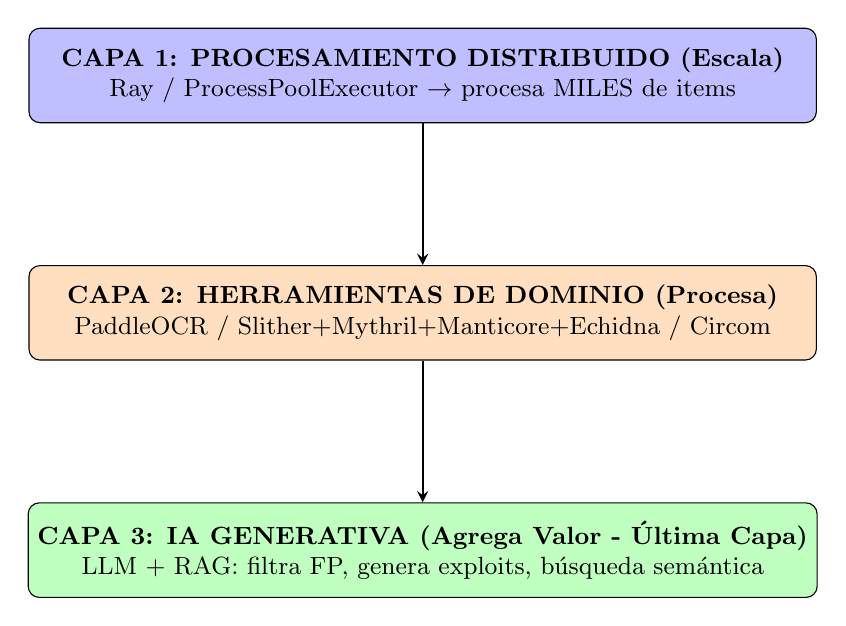
\begin{tikzpicture}[
    node distance=1.8cm,
    layer/.style={draw, rounded corners, minimum width=10cm, minimum height=1.2cm, align=center, font=\small},
    arrow/.style={->, thick, >=stealth}
]
    % Capa 1
    \node[layer, fill=blue!25] (dist) {
        \textbf{CAPA 1: PROCESAMIENTO DISTRIBUIDO (Escala)}\\
        Ray / ProcessPoolExecutor $\rightarrow$ procesa MILES de items
    };
    
    % Capa 2
    \node[layer, fill=orange!25, below=of dist] (tools) {
        \textbf{CAPA 2: HERRAMIENTAS DE DOMINIO (Procesa)}\\
        PaddleOCR / Slither+Mythril+Manticore+Echidna / Circom
    };
    
    % Capa 3
    \node[layer, fill=green!25, below=of tools] (ia) {
        \textbf{CAPA 3: IA GENERATIVA (Agrega Valor - Última Capa)}\\
        LLM + RAG: filtra FP, genera exploits, búsqueda semántica
    };
    
    % Flechas
    \draw[arrow] (dist) -- (tools);
    \draw[arrow] (tools) -- (ia);
    
\end{tikzpicture}
\caption{Patrón arquitectónico: Distribuido $\rightarrow$ Herramientas $\rightarrow$ IA Generativa}
\label{fig:patrón_arquitectónico}
\end{figure}

La \textbf{Capa de Procesamiento Distribuido} permite escalar el análisis a grandes volúmenes. Implementa el patrón Pure Dispatcher donde Ray y ProcessPoolExecutor coordinan el procesamiento de miles de documentos o contratos en paralelo. Esta capa resuelve el problema de escala.

La \textbf{Capa de Herramientas de Dominio} realiza el procesamiento especializado. Para documentos incluye PaddleOCR y Weaviate. Para contratos inteligentes incluye Slither, Mythril, Manticore, Echidna y Circom. Esta capa genera los datos que serán procesados por la IA.

La \textbf{Capa de IA Generativa} es la capa final que agrega valor. El LLM recibe los resultados de las herramientas y realiza comprensión semántica, filtrado de falsos positivos, generación automática de exploits, y búsqueda semántica mediante RAG. Esta capa transforma datos crudos en información accionable.

La Tabla \ref{tab:instanciacion_patrón} muestra como el patrón se instancia en los dos dominios del primer aporte.

\begin{table}[h]
\centering
\caption{Instanciacion del patrón arquitectónico (Aporte 1)}
\label{tab:instanciacion_patrón}
\begin{tabular}{p{3.5cm}p{5cm}p{5cm}}
\toprule
\textbf{Capa} & \textbf{Cap 3: Documentos} & \textbf{Cap 4: SENTINEL} \\
\midrule
\textbf{1. Distribuido} & Ray + ProcessPool & Ray + ProcessPool \\
\textbf{2. Herramientas} & PaddleOCR, Weaviate & Slither, Mythril, Manticore, Echidna, Circom \\
\textbf{3. IA (última)} & RAG + Embeddings & LLM filtra FP + genera exploits \\
\midrule
\textbf{Escala} & 11,368 páginas & Miles de contratos \\
\textbf{Metrica} & 69.9x speedup & -54\% FP, F1=0.86 \\
\bottomrule
\end{tabular}
\end{table}

El segundo aporte (Capítulo 5: Análisis Clínico) utiliza IA Generativa sin arquitectura distribuida significativa, demostrando que la IA Generativa tiene valor propio independiente de la escala.

\section{Contribuciones}

Esta tesis realiza tres aportes principales, cada uno de los cuales representa una contribución original al estado del conocimiento en su respectivo dominio. A diferencia de enfoques previos centrados exclusivamente en modelos o algoritmos aislados, la presente tesis aborda los problemas desde una perspectiva sistémica, integrando modelos de lenguaje dentro de arquitecturas distribuidas orientadas a entornos operativos reales.

\subsection{Aporte 1: Arquitectura Distribuida con IA Generativa cómo Última Capa}

Este aporte consiste en un patrón arquitectónico de tres capas donde la IA Generativa actúa cómo capa final que agrega valor semántico al procesamiento masivo. La contribución se distingue de trabajos previos en que posicióna la IA no cómo componente central que procesa todo, sino cómo capa de valor agregado que opera sobre resultados ya procesados por herramientas especializadas:

\begin{enumerate}[label=\textbf{1.\arabic*.}]
    \item \textbf{Patrón Pure Dispatcher para Escala:} Se introduce un patrón donde Ray y ProcessPoolExecutor coordinan el procesamiento distribuido, logrando factores de aceleración de 69.9x en documentos y permitiendo escalar el análisis a miles de contratos inteligentes.
    
    \item \textbf{IA Generativa cómo Última Capa en Documentos:} El sistema RAG con embeddings procesa los resultados del OCR distribuido, habilitando búsqueda semántica sobre 11,368 páginas procesadas en 4.3 minutos.
    
    \item \textbf{IA Generativa cómo Última Capa en SENTINEL:} El LLM recibe los hallazgos de cuatro herramientas de análisis (Slither, Mythril, Manticore, Echidna) ejecutadas en paralelo, filtra falsos positivos (-54\%), y genera automáticamente código de exploits ejecutables en Foundry.
\end{enumerate}

\subsection{Aporte 2: Defensa contra Coerción Física con IA Generativa (ZK Bank)}

Este aporte presenta una arquitectura de privacidad financiera que aborda el problema del ataque de llave inglesa de \$5:

\begin{enumerate}[label=\textbf{2.\arabic*.}]
    \item \textbf{Problema Original:} Se identifica que la criptografía es inútil bajo coerción física, un problema no resuelto por soluciones existentes.
    
    \item \textbf{Detección de Coerción con IA:} Se desarrolla un modelo de comportamiento que utiliza IA Generativa para detectar anomalías indicativas de coerción.
    
    \item \textbf{Respuestas Adaptativas:} El sistema escala sus protecciones según el nivel de riesgo detectado, desde verificación adicional hasta bloqueo total con alerta de emergencia.
    
    \item \textbf{Billeteras Señuelo Generadas por IA:} La IA genera historiales de transacciónes creíbles para billeteras falsas que enganan al atacante.
    
    \item \textbf{Integración ZK + IA:} Se combina privacidad criptográfica (zk-SNARKs) con inteligencia artificial para una defensa en profundidad.
\end{enumerate}

\subsection{Aporte 3: IA Generativa en Procesos Clínicos}

Este aporte demuestra la aplicabilidad de la IA Generativa en un dominio donde la arquitectura distribuida no es el factor determinante:

\begin{enumerate}[label=\textbf{3.\arabic*.}]
    \item \textbf{Sistema Deep Think + RAG para Análisis Terapéutico:} Se desarrolla un sistema que combina razonamiento profundo con generación aumentada por recuperación, utilizando las definiciones de la escala Kiel cómo conocimiento de dominio.
    
    \item \textbf{Validación contra Expertos Humaños:} El sistema alcanza 92\% de concordancia con evaluadores expertos en factores terapéuticos explícitos, identificando claramente los límites de la automatización en factores implícitos.
    
    \item \textbf{Framework de Validación IA vs Expertos:} Se desarrolla una métodología sistemática para comparar sistemas de IA contra juicio humano experto, aplicable a dominios donde el ground truth depende de evaluación subjetiva.
\end{enumerate}

\section{Publicaciones Derivadas}

Los resultados de esta tesis han sido públicados o enviados para su públicacion en los siguientes trabajos científicos:

\begin{enumerate}
    \item Gil-Costa, V., \textbf{Jaime, R.}, Cagnina, L., Errecalde, M. ``Parallel Architectures for Large-Scale Document Processing: Integrating OCR and RAG Pipelines''. \textit{The Journal of Supercomputing}, Springer Nature. Enviado, en proceso de revisión por pares.
    
    \item \textbf{Jaime, R.}, Cagnina, L., Errecalde, M., Taborda, A. ``Potencialidades de la IA en el Estudio de Procesos Terapéuticos Grupales: Un Enfoque Transdisciplinario''. Presentado en congreso nacional.
    
    \item \textbf{Jaime, R.}, Gil-Costa, V., Errecalde, M. ``SENTINEL: Distributed AI Platform for Smart Contract Security Analysis''. En preparación para sometimiento a revista internacional.
\end{enumerate}

Adicionalmente, componentes del sistema han sido presentados en seminarios internos del Laboratorio de Investigacion y Desarrollo en Inteligencia Computaciónal y han recibido retroalimentacion que contribuyó a su mejora.

\section{Organización de la Tesis}

La tesis se organiza en siete capítulos cuyo contenido se describe a continuacion, junto con un conjunto de apéndices que proporcionan información complementaria.

El \textbf{Capítulo 1}, correspondiente a la presente introducción, presenta el contexto y motivación de la investigación, formula el problema y las hipótesis, establece los objetivos generales y específicos, describe la métodología adoptada, y enumera las contribuciones originales.

El \textbf{Capítulo 2} proporciona el marco teórico necesario para comprender las contribuciones de la tesis. Se presentan los fundamentos de computación distribuida, incluyendo conceptos de paralelismo, el framework Ray, el modelo de actores, y ProcessPoolExecutor. Se introducen los conceptos de inteligencia artificial generativa, incluyendo modelos de lenguaje, generación aumentada por recuperación, y razonamiento profundo. Se describen los fundamentos de criptografía de conocimiento cero y se presenta el contexto de seguridad de contratos inteligentes.

El \textbf{Capítulo 3} presenta el primer caso de estudio (Aporte 1): arquitecturas paralelas para procesamiento masivo de documentos. Se describe la problemática del procesamiento documental a escala, se presenta el diseño de tres arquitecturas alternativas, se detallá el pipeline de extracción, y se reportan los resultados experimentales con un conjunto de datos de 11,368 páginas.

El \textbf{Capítulo 4} presenta el segundo caso de estudio (Aporte 1): la plataforma SENTINEL para análisis de seguridad de contratos inteligentes. Se describe la problemática de seguridad en el ecosistema DeFi, se presenta la arquitectura del sistema que integra múltiples motores con inteligencia artificial, y se reportan resultados de reducción de falsos positivos y puntaje F1.

El \textbf{Capítulo 5} presenta ZK Bank (Aporte 2): una arquitectura de privacidad financiera que aborda el problema del ataque de llave inglesa de \$5. Se describe como la IA Generativa permite detectar coerción física, generar respuestas adaptativas, y crear billeteras señuelo creíbles, resolviendo un problema que la criptografía sola no puede abordar.

El \textbf{Capítulo 6} presenta el tercer caso de estudio (Aporte 3): la aplicación de inteligencia artificial generativa al análisis de procesos terapéuticos grupales. Se describe el marco teórico clínico, incluyendo los factores terapéuticos y la escala Kiel. Se presenta la métodología del estudio y se reportan resultados de concordancia con evaluadores humanos.

El \textbf{Capítulo 7} sintetiza los resultados obtenidos en los tres aportes, valida las hipótesis planteadas, presenta el patrón arquitectónico abstraido, discute las limitaciones del trabajo, y propone direcciones de investigación futura.

Los \textbf{Apéndices} proporcionan información complementaria, incluyendo un glosario de términos técnicos, detalles del pipeline OCR, y las definiciones operativas de la escala Kiel.


%%%%%%%%%%%%%%%%%%%%%%%%%%%%%%%%%%%%%%%%%%%%%%%%%%%%%%%%%%%%%%%%%
% CAPÍTULO 2: MARCO TEÓRICO (EXPANDIDO)
%%%%%%%%%%%%%%%%%%%%%%%%%%%%%%%%%%%%%%%%%%%%%%%%%%%%%%%%%%%%%%%%%
\chapter{Marco Teorico}
\label{cap:marco_teórico}

Este capítulo presenta los fundamentos conceptuales necesarios para comprender las contribuciones de esta tesis. Los contenidos se organizan en cuatro secciones principales que abordan las tecnologías y conceptos fundamentales utilizados en los tres casos de estudio: computación distribuida, inteligencia artificial generativa, criptografía de conocimiento cero, y seguridad de contratos inteligentes.

\section{Computación Distribuida}

La computación distribuida se refiere al uso de múltiples sistemas computaciónales que trabajan de manera coordinada para resolver problemas que exceden la capacidad de un sistema individual. Esta sección presenta los fundamentos teóricos y las tecnologías específicas utilizadas en esta tesis.

\subsection{Fundamentos de Paralelismo}

El paralelismo computaciónal se fundamenta en la ejecución simultanea de múltiples tareas con el objetivo de reducir el tiempo total de procesamiento. Comprender sus principios teóricos es esencial para diseñar sistemas distribuidos efectivos.

\subsubsection{Taxonomía de Flynn}

La taxonomía de Flynn clasifica las arquitecturas computaciónales según el número de flujos de instrucciónes y datos que pueden procesar simultáneamente. Las cuatro categorías son SISD (Single Instruction, Single Data), correspondiente a computadoras secuenciales tradicionales; SIMD (Single Instruction, Múltiple Data), donde una instrucción se aplica simultáneamente a múltiples datos; MISD (Múltiple Instruction, Single Data), de interes principalmente teórico; y MIMD (Múltiple Instruction, Múltiple Data), que incluye la mayoría de los sistemas paralelos modernos.

Los sistemas desarrollados en esta tesis corresponden a la categoría MIMD, donde múltiples procesadores ejecutan diferentes instrucciónes sobre diferentes datos de forma independiente. Esta flexibilidad permite abordar problemas donde diferentes partes del trabajo requieren procesamiento diferente.

\subsubsection{Paralelismo de Datos versus Paralelismo de Tareas}

Se distinguen dos formas principales de paralelismo según como se divide el trabajo. El paralelismo de datos consiste en aplicar la misma operación simultáneamente a diferentes porciones de un conjunto de datos. Este enfoque es apropiado cuando se tiene un gran volumen de datos homogéneos que requieren procesamiento similar.

El paralelismo de tareas consiste en ejecutar diferentes operaciónes concurrentemente sobre los mismos o diferentes datos. Este enfoque es apropiado cuando el problema puede descomponerse en subtareas independientes con diferentes requisitos de procesamiento.

En la práctica, los sistemas complejos combinan ambas formas de paralelismo. El procesamiento de documentos desarrollado en esta tesis utiliza paralelismo de datos para procesar múltiples documentos simultáneamente, mientras que SENTINEL utiliza paralelismo de tareas para ejecutar diferentes herramientas de análisis concurrentemente.

\subsubsection{Ley de Amdahl y Ley de Gustafson}

La Ley de Amdahl, formulada por Gene Amdahl en 1967, establece un límite teórico para la aceleración que puede lograrse mediante paralelización. Si una fracción $p$ del programa puede ejecutarse en paralelo y la fracción restante $(1-p)$ debe ejecutarse secuencialmente, la aceleración máxima con $n$ procesadores está dada por:

\begin{equation}
S(n) = \frac{1}{(1-p) + \frac{p}{n}}
\label{eq:amdahl}
\end{equation}

Esta formulación tiene implicaciones importantes. Cuando $n$ tiende a infinito, la aceleración se apróxima a $\frac{1}{1-p}$, lo que significa que incluso con recursos infinitos, la aceleración está limitada por la fracción secuencial. Por ejemplo, si el 10\% del programa es inherentemente secuencial, la aceleración máxima teórica es 10x.

La Ley de Gustafson, formulada por John Gustafson en 1988, proporciona una perspectiva complementaria al observar que en la práctica, los usuarios frecuentemente escalan el tamaño del problema junto con los recursos disponibles. Bajo está perspectiva, la aceleración se define cómo:

\begin{equation}
S(n) = n - (1-p)(n-1) = 1 + (n-1)p
\label{eq:gustafson}
\end{equation}

Esta formulación indica que la aceleración puede crecer linealmente con el número de procesadores si el tamaño del problema crece proporcionalmente, manteniendo constante la fracción del tiempo dedicado a la porcion secuencial.

En el contexto de esta tesis, la Ley de Gustafson es más relevante porque los problemas abordados involucran conjuntos de datos grandes donde la fracción paralelizable domina ampliamente. El procesamiento de 11,368 páginas puede paralelizarse casi completamente, con overhead secuencial mínimo para coordinación.

\subsubsection{Métricas de Rendimiento Paralelo}

El rendimiento de sistemas paralelos se evalúa mediante varias métricas complementarias. El factor de aceleración o speedup se define como la razón entre el tiempo de ejecución secuencial y el tiempo de ejecución paralelo:

\begin{equation}
S = \frac{T_{secuencial}}{T_{paralelo}}
\end{equation}

La eficiencia mide que tan bien se utilizan los recursos disponibles, definiéndose como la razón entre el speedup y el número de procesadores:

\begin{equation}
E = \frac{S}{n}
\end{equation}

Una eficiencia de 1.0 (o 100\%) indica speedup lineal perfecto, donde duplicar los recursos reduce el tiempo a la mitad. En la práctica, la eficiencia es menor debido a overheads de comunicación, sincronización, y desbalance de carga.

La escalabilidad describe cómo cambia el rendimiento cuando se aumentan los recursos. Un sistema con escalabilidad fuerte mantiene eficiencia constante al aumentar el número de procesadores para un problema de tamaño fijo. Un sistema con escalabilidad débil mantiene eficiencia constante al aumentar el tamaño del problema proporcionalmente a los recursos.

\subsection{Framework Ray}

Ray es un framework de código abierto desarrollado inicialmente por el laboratorio RISELab de la Universidad de California en Berkeley para la construccion de aplicaciónes distribuidas. Su diseño se enfoca en simplicidad de uso, rendimiento, y flexibilidad para soportar diversos patrones de computación.

\subsubsection{Arquitectura de Ray}

La arquitectura de Ray se compone de varios componentes que trabajan coordinadamente. El driver es el proceso que ejecuta el programa principal y coordina la ejecución distribuida. Los workers son procesos que ejecutan tareas remotas en los nodos del cluster. El Global Control Store (GCS) mantiene metadatos del sistema incluyendo localización de objetos y estado de tareas. El object store local en cada nodo almacena objetos en memoria compartida para acceso eficiente.

Cuando se inicia una aplicación Ray, el driver se conecta al cluster y puede enviar tareas a cualquier nodo disponible. Las tareas se programan considerando localidad de datos, disponibilidad de recursos, y balanceo de carga. Los resultados se almacenan en object stores locales y se transfieren entre nodos según sea necesario.

\begin{figure}[h]
\centering
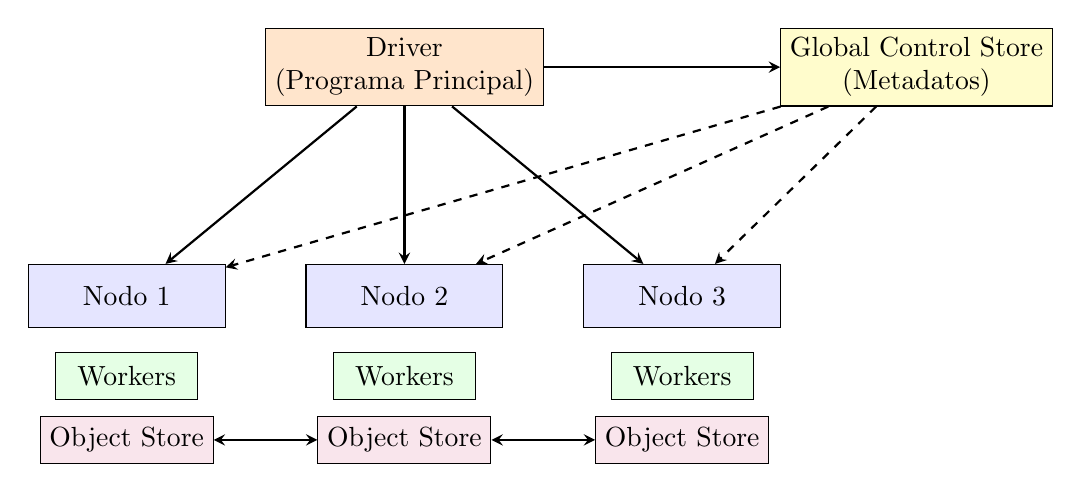
\begin{tikzpicture}[
    node distance=1.5cm,
    box/.style={rectangle, draw, minimum width=2.5cm, minimum height=0.8cm, align=center, fill=blue!10},
    smallbox/.style={rectangle, draw, minimum width=1.8cm, minimum height=0.6cm, align=center, fill=green!10},
    arrow/.style={->, >=stealth, thick}
]
% Driver
\node[box, fill=orange!20] (driver) {Driver\\(Programa Principal)};

% GCS
\node[box, right=3cm of driver, fill=yellow!20] (gcs) {Global Control Store\\(Metadatos)};

% Nodo 1
\node[box, below left=2cm and 0.5cm of driver] (nodo1) {Nodo 1};
\node[smallbox, below=0.3cm of nodo1] (worker1) {Workers};
\node[smallbox, below=0.2cm of worker1, fill=purple!10] (obj1) {Object Store};

% Nodo 2
\node[box, below=2cm of driver] (nodo2) {Nodo 2};
\node[smallbox, below=0.3cm of nodo2] (worker2) {Workers};
\node[smallbox, below=0.2cm of worker2, fill=purple!10] (obj2) {Object Store};

% Nodo 3
\node[box, below right=2cm and 0.5cm of driver] (nodo3) {Nodo 3};
\node[smallbox, below=0.3cm of nodo3] (worker3) {Workers};
\node[smallbox, below=0.2cm of worker3, fill=purple!10] (obj3) {Object Store};

% Conexiones
\draw[arrow] (driver) -- (gcs);
\draw[arrow] (driver) -- (nodo1);
\draw[arrow] (driver) -- (nodo2);
\draw[arrow] (driver) -- (nodo3);
\draw[arrow, dashed] (gcs) -- (nodo1);
\draw[arrow, dashed] (gcs) -- (nodo2);
\draw[arrow, dashed] (gcs) -- (nodo3);
\draw[arrow, <->] (obj1) -- (obj2);
\draw[arrow, <->] (obj2) -- (obj3);
\end{tikzpicture}
\caption{Arquitectura del framework Ray mostrando la relación entre el driver, el Global Control Store, y los nodos de trabajo con sus object stores locales.}
\label{fig:ray_architecture}
\end{figure}

\subsubsection{Tareas y Actores}

Ray proporciona dos abstracciones principales para programación distribuida: tareas y actores.

Las tareas en Ray representan funciones que pueden ejecutarse de forma remota en cualquier nodo del cluster. Una función se convierte en tarea remota mediante un decorador especial. Cuando se invoca una tarea remota, Ray serializa los argumentos, envía la solicitud al scheduler, ejecuta la función en un worker disponible, y retorna una referencia futura al resultado. El llamador puede continuar ejecutando código mientras la tarea se procesa remotamente, y obtener el resultado cuando lo necesite.

Este modelo simplifica significativamente el desarrollo de aplicaciónes paralelas porque el programador no necesita manejar explícitamente la comunicación entre nodos, la serialización de datos, ni la sincronización de resultados. Ray abstrae estos detalles y proporciona una interfaz que se asemeja a llamadas de funciones locales.

Los actores en Ray son objetos con estado que residen en un nodo específico del cluster y procesan métodos de forma secuencial. A diferencia de las tareas, que son sin estado y pueden ejecutarse en cualquier nodo, los actores mantienen su estado entre invocaciones de métodos. Esto los hace adecuados para escenarios donde se requiere mantener recursos costosos de inicializar, cómo modelos de aprendizaje automático cargados en memoria GPU.

Los actores se crean específicando una clase y sus parámetros de inicialización. Ray instancia el actor en un nodo apropiado y retorna una referencia que permite invocar métodos remotamente. Las invocaciones a métodos del mismo actor se procesan secuencialmente, garantizando consistencia del estado interno.

\subsubsection{Object Store y Transferencia de Datos}

Ray utiliza Apache Arrow cómo formato de serialización para objetos en memoria. El object store de cada nodo almacena objetos en memoria compartida, permitiendo acceso eficiente sin copias entre procesos del mismo nodo.

Cuando una tarea requiere datos que residen en otro nodo, Ray transfiere automáticamente los objetos necesarios. El scheduler considera la localidad de datos al asignar tareas, prefiriendo ejecutar tareas en nodos que ya tienen los datos requeridos. Esto reduce la transferencia de datos y mejora el rendimiento.

Para objetos grandes, Ray soporta streaming de datos que permite comenzar el procesamiento antes de que la transferencia complete. Esto es útil para pipelines donde etapas sucesivas pueden operar sobre datos parciales.

\subsubsection{Tolerancia a Fallos}

Ray proporciona tolerancia a fallos mediante reejecution automática de tareas fallidas. Cuando un worker fallá durante la ejecución de una tarea, el scheduler detecta el fallo y reprograma la tarea en otro worker disponible. Los argumentos de la tarea se reconstruyen desde el object store o mediante reejecución de las tareas que los produjeron.

Para actores, la tolerancia a fallos es más compleja porque involucra estado mutable. Ray soporta checkpointing de actores, donde el estado se guarda periódicamente y puede restaurarse tras un fallo. El programador puede configurar la frecuencia de checkpoints y el comportamiento ante fallos.

\subsection{Modelo de Actores y Akka}

El modelo de actores es un paradigma de computación concurrente donde los actores son las unidades fundamentales de computación. Propuesto originalmente por Carl Hewitt en 1973, el modelo ha ganado popularidad cómo alternativa a los modelos basados en memoria compartida y locks.

\subsubsection{Principios del Modelo de Actores}

En el modelo de actores, cada actor encapsula estado y comportamiento, y se comunica con otros actores exclusivamente mediante el envío de mensajes asíncronos. No existe memoria compartida entre actores, lo que elimina problemas de concurrencia cómo condiciones de carrera y deadlocks asociados con locks.

Cada actor tiene un buzon donde se almacenan mensajes entrantes. El actor procesa mensajes de su buzon uno a la vez, ejecutando comportamiento específico según el tipo de mensaje. El procesamiento de un mensaje puede resultar en envío de mensajes a otros actores, creacion de nuevos actores, o modificacion del estado interno del actor.

La asincronia del modelo permite alto grado de concurrencia. Un actor puede enviar un mensaje y continuar procesando sin esperar respuesta. Esto es especialmente útil en sistemas distribuidos donde la latencia de comunicación es significativa.

\subsubsection{Implementacion con Akka}

Akka es una implementación del modelo de actores para la plataforma JVM, soportando tanto Java cómo Scala. Proporciona abstracciones de alto nivel para construir sistemas concurrentes, distribuidos y tolerantes a fallos.

Los actores en Akka se definen cómo clases que extienden una clase base y específican su comportamiento mediante un método que describe cómo procesar diferentes tipos de mensajes. Los actores se crean mediante un sistema de actores que gestiona su ciclo de vida y comunicación.

Akka extiende el modelo básico de actores con caracteristicas adicionales. La supervisión jerárquica permite definir como los actores padre manejan fallos de sus hijos. Akka Cluster extiende actores a múltiples nodos con membership dinámico. Akka Persistence permite persistir el estado de actores para recuperación tras fallos.

\subsubsection{Comparación Ray versus Akka}

Ray y Akka representan diferentes aproximaciónes al problema de computación distribuida, cada una con fortalezas para diferentes escenarios.

Ray se enfoca en simplicidad de uso para aplicaciónes de datos y machine learning. Su modelo de tareas es más familiar para programadores acostumbrados a funciones, y su integración con Python lo hace accesible para la comunidad de ciencia de datos. Ray excele en escenarios donde el trabajo puede dividirse en tareas independientes que procesan datos de forma relativamente uniforme.

Akka se enfoca en sistemas reactivos con interacciónes complejas entre componentes. Su modelo de actores con estado es más apropiado para sistemas donde los componentes mantienen contexto entre interacciónes. Akka excele en sistemas de tiempo real, procesamiento de eventos, y aplicaciónes donde la consistencia eventual es aceptable.

En esta tesis, Ray se utiliza para el procesamiento de documentos donde las tareas son independientes y el modelo de tareas sin estado es apropiado. Akka se menciona cómo alternativa para SENTINEL donde la orquestación de múltiples herramientas con diferentes tiempos de respuesta se beneficia del modelo de actores.

\subsection{ProcessPoolExecutor}

ProcessPoolExecutor es una clase de la biblioteca estándar de Python que proporciona una interfaz de alto nivel para la ejecución paralela de tareas en múltiples procesos. Esta sección describe su funciónamiento y las consideraciones para su uso efectivo.

\subsubsection{Procesos versus Threads en Python}

Python presenta una limitación conocida cómo Global Interpreter Lock (GIL) que previene la ejecución simultanea de bytecode Python en múltiples threads del mismo proceso. Esto significa que aunque se utilicen múltiples threads, sólo uno puede ejecutar código Python en cualquier momento.

Para tareas limitadas por CPU, como el procesamiento de imágenes o cálculos numéricos, los threads no proporcionan paralelismo real. La solución es utilizar múltiples procesos, cada uno con su propio intérprete Python y por tanto su propio GIL. ProcessPoolExecutor facilita este patrón.

Para tareas limitadas por I/O, cómo acceso a red o disco, los threads pueden ser efectivos porque el GIL se libera durante operaciónes de I/O. Sin embargo, para el procesamiento de documentos con OCR, que es intensivo en CPU, los procesos separados son necesarios.

\subsubsection{Funciónamiento de ProcessPoolExecutor}

ProcessPoolExecutor mantiene un pool de procesos trabajadores que se crean al inicializar el executor y permanecen activos esperando trabajo. Cuando se envía una tarea al executor, este serializa la función y sus argumentos, envía los datos a un proceso trabajador disponible, espera el resultado, y lo deserializa para retornarlo al llamador.

La interfaz principal consiste en dos métodos. El método submit envía una tarea individual y retorna un objeto Future que representa el resultado pendiente. El método map aplica una función a una secuencia de argumentos, similar a la función map incorporada pero ejecutando en paralelo.

El número de procesos en el pool es configurable. Por defecto se utiliza el número de CPUs disponibles. Para tareas que utilizan GPU, puede ser apropiado utilizar menos procesos si la GPU es el recurso limitante.

\subsubsection{Inicializadores de Procesos}

Una caracteristica importante de ProcessPoolExecutor es la capacidad de específicar una función inicializadora que se ejecuta una vez en cada proceso trabajador antes de procesar tareas. Esto es útil para cargar recursos costosos cómo modelos de machine learning.

En el contexto de esta tesis, el inicializador se utiliza para cargar el modelo de PaddleOCR en cada proceso trabajador. Sin está optimización, el modelo se cargaría cada vez que se procesa un documento, desperdiciando varios segundos por documento. Con el inicializador, la carga ocurre una sola vez por proceso, y todas las tareas subsiguientes reutilizan el modelo cargado.

\subsubsection{Consideraciones de Memoria}

Cada proceso trabajador tiene su propio espacio de memoria. Cuando se envian datos a un proceso, estos se serializan mediante pickle y se copian al espacio de memoria del proceso. Para datos grandes, esto puede resultar en uso significativo de memoria y tiempo de transferencia.

Estrategias para mitigar estos problemas incluyen enviar referencias a archivos en lugar de datos en memoria, utilizar memoria compartida para datos de sólo lectura, y diseñar tareas que procesen datos en lotes apropiados.

\section{Inteligencia Artificial Generativa}

La inteligencia artificial generativa se refiere a sistemas capaces de crear contenido nuevo basándose en patrones aprendidos de datos de entrenamiento. Esta sección presenta los fundamentos de los modelos de lenguaje y las técnicas de aumentación que se utilizan en esta tesis.

\subsection{Modelos de Lenguaje de Gran Escala}

Los modelos de lenguaje de gran escala, conocidos por sus siglas en ingles LLM (Large Language Models), representan uno de los avances más significativos en inteligencia artificial de la última década. Su capacidad para comprender y generar texto los hace aplicables a una amplia gama de tareas.

\subsubsection{Arquitectura Transformer}

La arquitectura Transformer, introducida por Vaswani y colaboradores en 2017, constituye la base de los modelos de lenguaje modernos. Su innovacion principal es el mecanismo de atención que permite al modelo considerar todas las posiciónes de una secuencia simultáneamente, en contraste con arquitecturas recurrentes que procesan secuencias posición por posición.

El mecanismo de atención calcula la relevancia de cada posición de la secuencia para predecir cada otra posición. Formalmente, dadas matrices de consultas Q, claves K, y valores V, la atención se calcula cómo:

\begin{equation}
Attention(Q,K,V) = softmax\left(\frac{QK^T}{\sqrt{d_k}}\right)V
\end{equation}

donde $d_k$ es la dimensión de las claves. El factor de escala $\sqrt{d_k}$ previene que los productos punto crezcan demasiado para dimensiones grandes.

Los Transformers utilizan atención multi-cabeza, donde múltiples funciones de atención operan en paralelo sobre diferentes proyecciones de la entrada. Esto permite al modelo atender a diferentes tipos de relaciónes simultáneamente.

\subsubsection{Preentrenamiento y Ajuste Fino}

El entrenamiento de modelos de lenguaje típicamente ocurre en dos fases. La primera fase, denominada preentrenamiento, consiste en entrenar el modelo para predecir texto en grandes corpus no etiquetados. El objetivo puede ser predecir la siguiente palabra dada el contexto precedente, predecir palabras enmascaradas en el contexto, o una combinación de objetivos.

Durante el preentrenamiento, el modelo aprende representaciónes del lenguaje que capturan sintaxis, semántica, y conocimiento del mundo. Los corpus de entrenamiento incluyen texto de la web, libros, artículos científicos, y código. Los modelos más grandes utilizan trillones de tokens de entrenamiento.

La segunda fase, denominada ajuste fino o alíneación, adapta el modelo para seguir instrucciónes y producir respuestas útiles y seguras. Técnicas cómo RLHF (Reinforcement Learning from Human Feedback) utilizan retroalimentacion humana para entrenar el modelo a producir respuestas preferidas.

\subsubsection{Capacidades Emergentes}

Los modelos de lenguaje de gran escala exhiben capacidades emergentes que no están presentes en modelos más pequeños. Estas capacidades aparecen a partir de ciertos umbrales de tamaño y parecen surgir de forma no gradual.

El razonamiento de múltiples pasos permite al modelo resolver problemas que requieren secuencias de inferencias. La comprensión de contexto extenso permite procesar y relaciónar información de documentos largos. La generación de código permite producir programas funcionales a partir de descripciónes en lenguaje natural.

Estas capacidades hacen a los modelos de lenguaje aplicables a tareas que requieren comprensión semántica profunda, como el análisis de documentos, la evaluación de código, y la asistencia en decisiones clínicas.

\subsection{Generación Aumentada por Recuperacion}

La Generación Aumentada por Recuperacion, conocida por sus siglas en ingles RAG (Retrieval-Augmented Generation), es una técnica que combina la recuperación de información con la generación de texto para mejorar la precisión y fundamentacion de las respuestas.

\subsubsection{Motivación}

Los modelos de lenguaje tienen conocimiento limitado por sus datos de entrenamiento. Información posterior al entrenamiento no está disponible, y detalles específicos pueden no estar representados adecuadamente. Adicionalmente, los modelos pueden generar información plausible pero incorrecta, fenómeno conocido cómo alucinación.

RAG aborda estas limitaciones proporcionando al modelo acceso a una base de conocimientos externa durante la generación. En lugar de depender exclusivamente de conocimiento paramétrico, el modelo puede consultar documentos relevantes y basar sus respuestas en información verificable.

\subsubsection{Proceso de RAG}

El procesó típico de RAG consiste en tres etapas principales.

En la primera etapa, la consulta del usuario se convierte en un vector denso mediante un modelo de embeddings. Este modelo proyecta el texto a un espacio de alta dimensión donde textos semánticamente similares tienen vectores cercanos.

En la segunda etapa, el vector de la consulta se utiliza para buscar documentos similares en una base de datos vectorial. La búsqueda retorna los k documentos más cercanos según alguna métrica de distancia, típicamente distancia coseno o producto interno.

En la tercera etapa, los documentos recuperados se incluyen en el contexto del modelo de lenguaje junto con la consulta original. El modelo genera una respuesta basada tanto en su conocimiento interno cómo en la información de los documentos recuperados.

\begin{figure}[h]
\centering
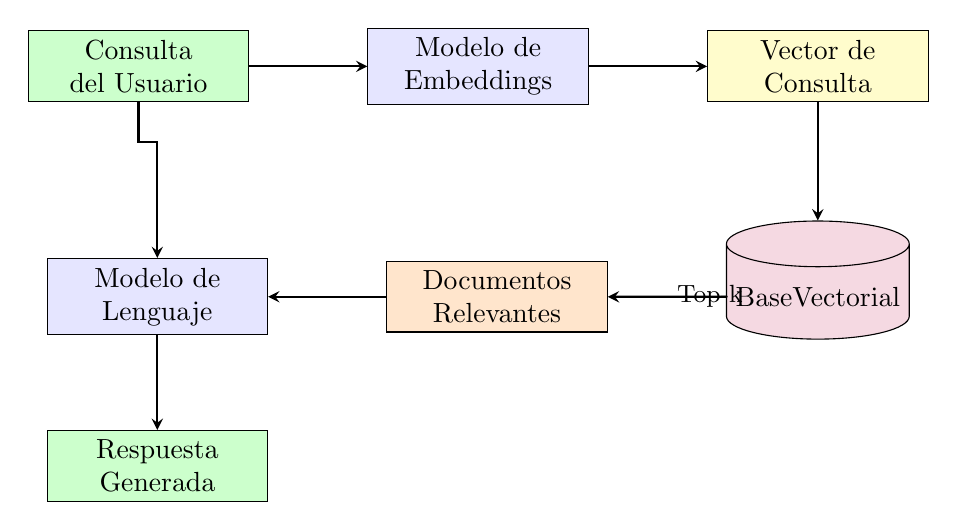
\begin{tikzpicture}[
    node distance=1.2cm,
    box/.style={rectangle, draw, minimum width=2.8cm, minimum height=0.8cm, align=center, fill=blue!10},
    db/.style={cylinder, draw, shape border rotate=90, aspect=0.25, minimum height=1.5cm, minimum width=1.2cm, fill=purple!15},
    arrow/.style={->, >=stealth, thick}
]
% Query
\node[box, fill=green!20] (query) {Consulta\\del Usuario};

% Embedding model
\node[box, right=1.5cm of query] (embed) {Modelo de\\Embeddings};

% Vector
\node[box, right=1.5cm of embed, fill=yellow!20] (vector) {Vector de\\Consulta};

% Vector DB
\node[db, below=1.5cm of vector] (db) {Base\\Vectorial};

% Retrieved docs
\node[box, left=1.5cm of db, fill=orange!20] (docs) {Documentos\\Relevantes};

% LLM
\node[box, left=1.5cm of docs] (llm) {Modelo de\\Lenguaje};

% Response
\node[box, below=1.2cm of llm, fill=green!20] (response) {Respuesta\\Generada};

% Arrows
\draw[arrow] (query) -- (embed);
\draw[arrow] (embed) -- (vector);
\draw[arrow] (vector) -- (db);
\draw[arrow] (db) -- node[right, font=\small] {Top-k} (docs);
\draw[arrow] (docs) -- (llm);
\draw[arrow] (query.south) -- ++(0,-0.5) -| (llm.north);
\draw[arrow] (llm) -- (response);
\end{tikzpicture}
\caption{Arquitectura de Generación Aumentada por Recuperacion (RAG) mostrando el flujo desde la consulta del usuario hasta la respuesta generada, pasando por la recuperación de documentos relevantes.}
\label{fig:rag_architecture}
\end{figure}

\subsubsection{Embeddings y Bases de Datos Vectoriales}

Los embeddings son representaciónes vectoriales densas de texto que capturan significado semántico. Modelos especializados cómo Sentence-BERT, OpenAI ada-002, y alternativas de código abierto producen embeddings donde la similitud coseno entre vectores correlacióna con la similitud semántica del texto.

Las bases de datos vectoriales cómo Weaviate, Pinecone, Milvus, y Qdrant están optimizadas para almacenar grandes cantidades de vectores y realizar búsquedas de similitud eficientes. Utilizan estructuras de datos especializadas cómo HNSW (Hierarchical Navigable Small World) para encontrar vecinos cercanos en tiempo sublineal.

En esta tesis, Weaviate se utiliza cómo base de datos vectorial para el sistema de procesamiento de documentos. Los fragmentos de texto extraído se convierten en embeddings y se almacenan en Weaviate, permitiendo búsquedas semánticas sobre el corpus completo.

\subsubsection{Ventajas de RAG}

RAG presenta varias ventajas sobre los modelos de lenguaje tradicionales.

La actúalización del conocimiento no requiere reentrenar el modelo. Agregar nuevos documentos a la base de conocimientos los hace inmediatamente disponibles para consulta. Esto es crítico para dominios donde la información cambia frecuentemente.

La trazabilidad permite identificar las fuentes utilizadas para generar una respuesta. Esto facilita la verificación y aumenta la confianza en las respuestas. Los usuarios pueden consultar los documentos originales para profundizar.

La reducción de alucinaciones resulta de anclar las respuestas en documentos verificables. Cuando el modelo basa su respuesta en texto recuperado, es menos probable que genere información incorrecta.

\subsection{Razónamiento Profundo}

El razonamiento profundo, conocido comercialmente cómo Deep Think en algunos modelos, es una capacidad que permite a los modelos de lenguaje analizar problemas de forma más exhaustiva antes de producir una respuesta.

\subsubsection{Concepto}

En el modo de razonamiento profundo, el modelo no produce una respuesta inmediata. En cambio, genera una secuencia de pasos de razonamiento que exploran diferentes aspectos del problema, consideran alternativas, y evalúan la consistencia de diferentes interpretaciones.

Este proceso es análogo a como un experto humano abordaría un problema complejo: considerando múltiples perspectivas, evaluando evidencia a favor y en contra de diferentes conclusiones, y refinando su análisis antes de comprometerse con una respuesta.

\subsubsection{Aplicaciones}

El razonamiento profundo es particularmente útil en tareas donde la respuesta correcta no es obvia y requiere considerar múltiples factores. Ejemplos incluyen problemas matemáticos complejos, análisis de situaciones ambiguas, y evaluación de textos donde el significado depende del contexto.

En el sistema de análisis clínico desarrollado en esta tesis, el razonamiento profundo se utiliza para evaluar transcripciones de sesiónes terapéuticas. El modelo considera cómo diferentes fragmentos de la sesión se relaciónan con los factores terapéuticos, evalúa interpretaciones alternativas, y produce puntuaciónes que reflejan un análisis exhaustivo.

\subsubsection{Limitaciones}

El razonamiento profundo tiene limitaciones que deben considerarse. El tiempo de respuesta es significativamente mayor que en generación directa. El costo computaciónal es proporcional a la longitud del razonamiento. Y aunque el razonamiento profundo mejora la calidad en muchos casos, no garantiza respuestas correctas.

\section{Criptografía de Conocimiento Cero}

Las pruebas de conocimiento cero son protocolos criptográficos que permiten demostrar la veracidad de una afirmación sin revelar información adicional. Esta sección presenta los fundamentos teóricos y las tecnologías utilizadas en el módulo ZK Bank.

\subsection{Fundamentos Teoricos}

\subsubsection{Definición Formal}

Un protocolo de conocimiento cero involucra dos partes: un probador que desea demostrar conocimiento de información secreta, y un verificador que desea convencerse de la veracidad de una afirmación sin aprender la información secreta.

Formalmente, un protocolo de conocimiento cero debe satisfacer tres propiedades:

\textbf{Completitud:} Si la afirmación es verdadera, un probador honesto puede convencer a un verificador honesto. Matemáticamente, si $x \in L$ donde L es el lenguaje de afirmaciones verdaderas, entonces la probabilidad de que el verificador acepte es cercana a 1.

\textbf{Solidez:} Si la afirmación es falsa, ningún probador puede convencer al verificador excepto con probabilidad negligible. Matemáticamente, si $x \notin L$, entonces la probabilidad de que el verificador acepte es cercana a 0.

\textbf{Conocimiento cero:} El verificador no aprende nada más allá de la veracidad de la afirmación. Formalmente, existe un simulador que puede producir transcripciones indistinguibles de interacciónes reales sin conocer el secreto del probador.

\subsubsection{Tipos de Pruebas de Conocimiento Cero}

Las pruebas de conocimiento cero se clasifican según varias dimensiones.

Según la interactividad, las pruebas interactivas requieren comunicación de ida y vuelta entre probador y verificador, mientras que las pruebas no interactivas consisten en un único mensaje del probador al verificador.

Según el tipo de solidez, las pruebas pueden tener solidez estadística, donde la probabilidad de error es negligible para cualquier probador computaciónalmente ilimitado, o solidez computaciónal, donde la solidez depende de suposiciónes sobre la dificultad de ciertos problemas.

Según el setup, algunos protocolos requieren una fase de configuración confiable donde se generan parámetros públicos, mientras que otros protocolos son transparentes y no requieren setup confiable.

\subsection{zk-SNARKs}

Los zk-SNARKs (Zero-Knowledge Succinct Non-Interactive Arguments of Knowledge) son un tipo específico de prueba de conocimiento cero con propiedades que los hacen particularmente adecuados para aplicaciónes blockchain.

\subsubsection{Propiedades}

Los zk-SNARKs se caracterizan por varias propiedades deseables:

\textbf{Sucintez:} Las pruebas son de tamaño constante independientemente del tamaño de la computación que verifican. Una prueba tipica ocupa unos pocos cientos de bytes.

\textbf{No interactividad:} La prueba consiste en un único mensaje del probador al verificador, lo que permite verificación sin comunicación.

\textbf{Verificacion rápida:} Verificar una prueba requiere tiempo constante o logaritmico en el tamaño de la computación, significativamente menos que ejecutar la computación directamente.

Estas propiedades hacen a los zk-SNARKs adecuados para blockchain, donde las pruebas deben almacenarse en la cadena y verificarse por todos los nodos.

\begin{figure}[h]
\centering
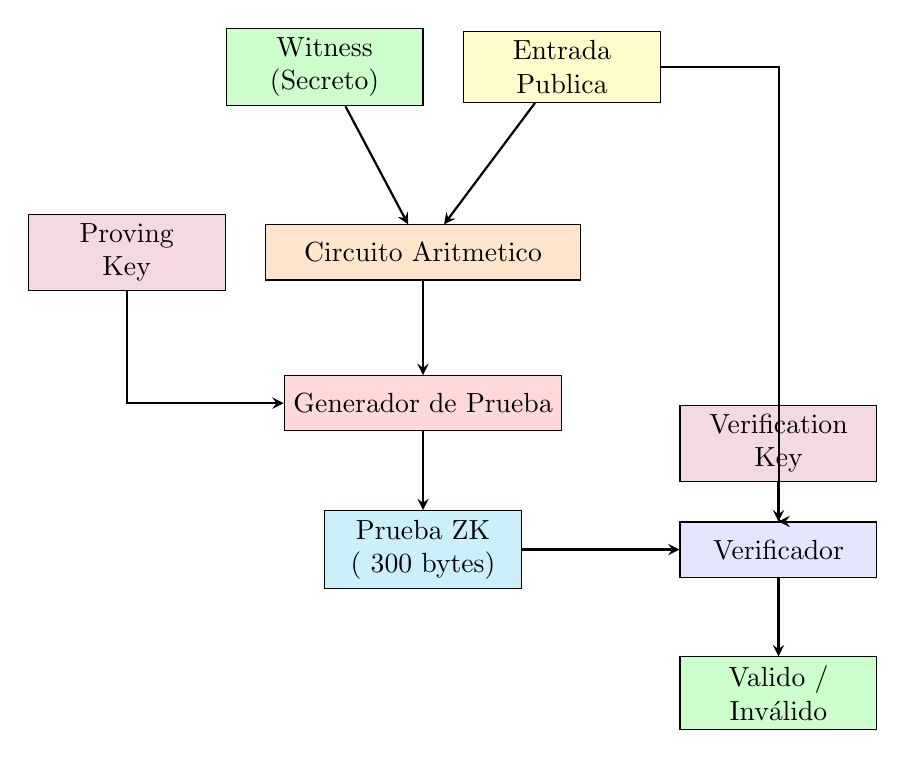
\begin{tikzpicture}[
    node distance=1cm,
    box/.style={rectangle, draw, minimum width=2.5cm, minimum height=0.7cm, align=center, fill=blue!10},
    arrow/.style={->, >=stealth, thick}
]
% Inputs
\node[box, fill=green!20] (witness) {Witness\\(Secreto)};
\node[box, right=0.5cm of witness, fill=yellow!20] (public) {Entrada\\Publica};

% Circuit
\node[box, below=1.5cm of witness, xshift=1.25cm, minimum width=4cm, fill=orange!20] (circuit) {Circuito Aritmetico};

% Proving key
\node[box, left=0.5cm of circuit, fill=purple!15] (pk) {Proving\\Key};

% Proof generation
\node[box, below=1.2cm of circuit, fill=red!15] (prover) {Generador de Prueba};

% Proof
\node[box, below=1cm of prover, fill=cyan!20] (proof) {Prueba ZK\\(~300 bytes)};

% Verification
\node[box, right=2cm of proof] (verifier) {Verificador};

% VK
\node[box, above=0.5cm of verifier, fill=purple!15] (vk) {Verification\\Key};

% Result
\node[box, below=1cm of verifier, fill=green!20] (result) {Valido /\\Inválido};

% Arrows
\draw[arrow] (witness) -- (circuit);
\draw[arrow] (public) -- (circuit);
\draw[arrow] (circuit) -- (prover);
\draw[arrow] (pk) |- (prover);
\draw[arrow] (prover) -- (proof);
\draw[arrow] (proof) -- (verifier);
\draw[arrow] (vk) -- (verifier);
\draw[arrow] (public.east) -- ++(1.5,0) |- (verifier.north);
\draw[arrow] (verifier) -- (result);
\end{tikzpicture}
\caption{Flujo de generación y verificación de pruebas zk-SNARK. El probador genera una prueba compacta a partir del witness secreto y la entrada pública, mientras el verificador puede validar la prueba sin conocer el secreto.}
\label{fig:zksnark_flow}
\end{figure}

\subsubsection{Construccion}

La construccion de zk-SNARKs típicamente involucra varios pasos.

Primero, la computación a probar se expresa como un circuito aritmetico sobre un campo finito. El circuito consiste en compuertas de suma y multiplicacion conectadas por cables que transportan valores del campo.

Segundo, el circuito se transforma en un sistema de restricciones cuadraticas (QAP o R1CS). Cada restriccion es una ecuacion cuadratica que los valores de los cables deben satisfacer.

Tercero, se ejecuta una ceremonia de setup que genera claves de prueba y verificación a partir del sistema de restricciones. La seguridad depende de que los parámetros secretos usados en el setup sean descartados.

Cuarto, el probador utiliza la clave de prueba junto con sus entradas privadas para generar una prueba. La prueba es un conjunto de elementos de curva elíptica que codifican conocimiento del testigo sin revelarlo.

Quinto, el verificador utiliza la clave de verificación y las entradas públicas para verificar la prueba mediante un número constante de operaciónes de emparejamiento en curvas elípticas.

\subsection{Circom}

Circom es un lenguaje de dominio específico para definir circuitos aritmeticos que pueden compilarse a zk-SNARKs. Su diseño enfatiza expresividad y fácilidad de uso para desarrolladores.

\subsubsection{Modelo de Programacion}

En Circom, los circuitos se definen mediante templates que específican señales de entrada y salida, señales intermedias, y restricciones entre ellas.

Las señales representan valores del campo finito. Las señales de entrada pueden ser públicas, conocidas por el verificador, o privadas, conocidas sólo por el probador. Las señales de salida son típicamente públicas y representan el resultado de la computación.

Las restricciones son ecuaciones cuadraticas que las señales deben satisfacer. El compilador de Circom verifica que las restricciones son satisfacibles y genera los artefactos necesarios para crear y verificar pruebas.

\subsubsection{Componentes}

Circom soporta modularidad mediante templates parametrizados que pueden instanciarse múltiples veces. Los templates pueden invocar otros templates, permitiendo construir circuitos complejos a partir de componentes simples.

La biblioteca circomlib proporciona implementaciónes optimizadas de operaciónes comunes, incluyendo funciones hash cómo Poseidon y MiMC, operaciónes de curva elíptica, y comparadores.

\subsubsection{Flujo de Trabajo}

El flujo de trabajo típico con Circom incluye varios pasos.

Primero, se escribe el circuito en lenguaje Circom específicando señales y restricciones. Se ejecutan pruebas con entradas conocidas para verificar el comportamiento.

Segundo, se compila el circuito para generar el sistema de restricciones en formato R1CS y el código para calcular el testigo.

Tercero, se ejecuta la ceremonia de setup utilizando herramientas cómo snarkjs o rapidsnark. Para circuitos de producción, se utilizan ceremonias de Powers of Tau con múltiples participantes.

Cuarto, el probador calcula el testigo ejecutando el circuito con sus entradas, y genera la prueba utilizando la clave de prueba.

Quinto, el verificador verifica la prueba utilizando la clave de verificación. Para verificación en blockchain, se genera un contrato Solidity que implementa el verificador.

\section{Seguridad de Contratos Inteligentes}

Los contratos inteligentes son programas que se ejecutan en plataformas blockchain y controlan activos digitales. Esta sección presenta el contexto de seguridad y las herramientas utilizadas en SENTINEL.

\subsection{Contexto de Seguridad en DeFi}

\subsubsection{Ecosistema DeFi}

Las finanzas descentralizadas (DeFi) constituyen un ecosistema de aplicaciónes financieras construidas sobre plataformas blockchain, principalmente Ethereum. El valor total bloqueado en protocolos DeFi ha alcanzado decenas de miles de millones de dólares, creando incentivos significativos para atacantes.

Los protocolos DeFi incluyen intercambios descentralizados que permiten intercambiar tokens sin intermediarios, protocolos de prestamo que permiten depositar colateral y tomar prestamos, agregadores de rendimiento que optimizan retornos automáticamente, y puentes que permiten transferir activos entre blockchains.

\subsubsection{Caracteristicas que Amplifican Riesgos}

Varias caracteristicas del ecosistema DeFi amplifican los riesgos de seguridad.

La inmutabilidad significa que una vez desplegado, un contrato no puede modificarse. Las vulnerabilidades no pueden corregirse sin migrar a un nuevo contrato, procesó complejo que puede requerir movimiento de fondos de usuarios.

La irreversibilidad de transacciónes significa que los fondos robados no pueden recuperarse mediante mecanismos tradicionales. A diferencia de sistemas financieros tradicionales donde las transacciónes fraudulentas pueden revertirse, en blockchain las transacciónes son finales.

La composabilidad permite que contratos interactuen entre si de formas no anticipadas por sus desarrolladores. Un contrato seguro en aislamiento puede ser vulnerable cuando se combina con otros contratos.

El código abierto permite que atacantes analicen el código en busca de vulnerabilidades. Aunque la transparencia tiene beneficios, también facilita el descubrimiento de exploits.

\subsection{Vulnerabilidades Comúnes}

\subsubsection{Reentrada}

La reentrada es una vulnerabilidad donde un contrato malicioso puede llamar repetidamente a una función del contrato víctima antes de que se actualice el estado. El ataque clásico ocurre cuando un contrato envía Ether a una dirección externa antes de actualizar el balance del remitente.

El atacante despliega un contrato con una función de recepción que llama de vuelta al contrato víctima. Cuando la víctima envía Ether al atacante, la función de recepción se ejecuta y reinicia el procesó de retiro antes de que el balance se actualice, drenando los fondos del contrato.

La prevención incluye actualizar el estado antes de realizar llamadas externas, utilizar el patrón checks-effects-interactions, y emplear guardias de reentrada que previenen llamadas recursivas.

\subsubsection{Desbordamiento de Enteros}

El desbordamiento de enteros ocurre cuando una operación aritmética produce un resultado fuera del rango representable. En versiones antiguas de Solidity, estas operaciónes envolvían silenciosamente, produciendo resultados incorrectos.

Por ejemplo, si un uint8 con valor 255 se incrementa, el resultado es 0 en lugar de 256. Un atacante podría explotar esto para manipular balances o evadir validaciónes.

A partir de Solidity 0.8, las operaciónes aritméticas incluyen verificaciones automáticas que revierten la transacción en caso de desbordamiento. Sin embargo, contratos antiguos o aquellos que utilizan bloques unchecked permanecen vulnerables.

\subsubsection{Control de Acceso}

Las vulnerabilidades de control de acceso permiten que funciones críticas sean invocadas por actores no autorizados. Ejemplos incluyen funciones administrativas sin modificadores de acceso, uso incorrecto de tx.origin en lugar de msg.sender para autenticación, y falta de validación de parámetros de inicialización.

La prevención incluye utilizar modificadores de acceso consistentemente, preferir msg.sender sobre tx.origin, y validar que funciones de inicialización sólo puedan ejecutarse una vez.

\subsubsection{Manipulacion de Oraculos}

Los oráculos proporcionan datos externos a contratos inteligentes, cómo precios de activos. Los ataques de manipulación de oráculos explotan la confianza en estos datos para beneficio del atacante.

Los ataques de prestamos flash permiten tomar prestadas grandes cantidades de activos sin colateral si se devuelven en la misma transacción. Un atacante puede usar un prestamo flash para manipular temporalmente el precio en un exchange, explotar un protocolo que depende de ese precio, y devolver el prestamo con ganancias.

La prevención incluye utilizar oráculos resistentes a manipulación cómo Chainlink, promediar precios sobre múltiples bloques, y limitar el impacto de cambios bruscos de precio.

\subsection{Herramientas de Análisis}

\subsubsection{Slither}

Slither es un framework de análisis estático para Solidity desarrollado por Trail of Bits. Examina el código fuente sin ejecutarlo, construyendo representaciónes intermedias que facilitan la detección de patrones vulnerables.

Slither construye un árbol de sintaxis abstracta (AST) del código fuente, lo transforma en una representación intermedia llamada SlithIR, y ejecuta detectores sobre está representación. Los detectores identifican patrones asociados con vulnerabilidades conocidas, malas prácticas, y oportunidades de optimización.

Las fortalezas de Slither incluyen su velocidad, que permite analizar contratos en segundos, su amplia cobertura con más de 80 detectores, y su capacidad de extensión mediante detectores personalizados. Sus limitaciones incluyen la incapacidad de detectar vulnerabilidades que dependen del estado de ejecución y la generación de falsos positivos que requieren revisión manual.

\subsubsection{Mythril}

Mythril es una herramienta de análisis de seguridad que utiliza ejecución simbólica para explorar caminos de ejecución posibles. En lugar de ejecutar el contrato con valores concretos, utiliza variables simbólicas y resuelve restricciones para determinar que entradas pueden alcanzar estados vulnerables.

Mythril analiza bytecode compilado, lo que permite analizar contratos desplegados sin acceso al código fuente. Utiliza el motor Z3 para resolver restricciones y determinar la satisfacibilidad de condiciones.

Las fortalezas de Mythril incluyen su capacidad para detectar vulnerabilidades que dependen de valores específicos de entrada y su independencia del código fuente. Sus limitaciones incluyen tiempos de análisis largos para contratos complejos y la posibilidad de no explorar todos los caminos debido a explosion combinatoria.

\subsubsection{Manticore}

Manticore es otra herramienta de ejecución simbólica desarrollada por Trail of Bits. Complementa a Mythril utilizando diferentes estrategias de exploración del espacio de estados.

Manticore soporta análisis de contratos Ethereum y binarios x86/ARM. Para Ethereum, puede analizar tanto bytecode cómo código fuente con información de debug.

Las fortalezas de Manticore incluyen su profundidad de análisis y su capacidad para generar casos de prueba concretos que demuestran vulnerabilidades. Sus limitaciones son similares a Mythril en términos de tiempo de análisis y explosion combinatoria.

\subsubsection{Echidna}

Echidna es un fuzzer basado en propiedades específicamente diseñado para contratos inteligentes. En lugar de buscar crashes cómo fuzzers tradicionales, Echidna intenta violar propiedades definidas por el usuario.

El usuario define propiedades cómo funciones que retornan un booleano. Echidna genera secuencias de transacciónes aleatorias y verifica que las propiedades se mantienen. Cuando encuentra una secuencia que viola una propiedad, reporta el contraejemplo.

Las fortalezas de Echidna incluyen su efectividad para encontrar vulnerabilidades en lógica de negocio y su capacidad para descubrir secuencias de transacciónes complejas que llevan a estados vulnerables. Sus limitaciones incluyen la necesidad de definir propiedades manualmente y la posibilidad de no alcanzar estados vulnerables si la exploración no es suficientemente exhaustiva.

\section{Trabajos Relaciónados}

Esta sección presenta un análisis de los trabajos previos más relevantes en cada una de las áreas abordadas por esta tesis, identificando sus contribuciones y las brechas que motivan la presente investigación.

\subsection{Procesamiento Distribuido de Documentos}

El procesamiento de documentos a gran escala ha sido abordado mediante diversas arquitecturas. Apache Spark ha sido utilizado extensivamente para procesamiento de texto distribuido, con trabajos como los de Zaharía et al. que demuestran su efectividad para análisis de logs y extracción de información. Sin embargo, estos enfoques típicamente asumen texto ya digitalizado y no abordan el desafío del OCR.

En el ámbito de OCR distribuido, Tesseract ha sido paralelizado mediante MapReduce en varios trabajos, logrando mejoras de rendimiento significativas. No obstante, estos enfoques no integran la extracción con sistemas de búsqueda semántica ni aprovechan modelos de lenguaje para post-procesamiento.

Trabajos recientes han explorado la integración de OCR con pipelines de RAG. LangChain y LlamaIndex proporcionan frameworks para construir estos pipelines, pero su enfoque está orientado a la funcionalidad más que al rendimiento, y no documentan estrategias de paralelización efectivas.

La brecha identificada es la ausencia de arquitecturas que integren OCR, post-procesamiento con IA, y búsqueda semántica en un pipeline distribuido optimizado para rendimiento. El Aporte 1 de esta tesis aborda está brecha mediante el patrón Pure Dispatcher.

\subsection{Análisis de Seguridad de Smart Contracts con IA}

Las herramientas tradicionales de análisis de smart contracts, incluyendo Slither, Mythril, Manticore y Echidna, han demostrado efectividad individual pero presentan altas tasas de falsos positivos cuando se usan en aislamiento. Trabajos cómo SmartCheck y Securify han propuesto enfoques alternativos basados en patrones, con resultados mixtos.

La aplicación de aprendizaje automático a la detección de vulnerabilidades ha sido explorada en varios trabajos. Qian et al. propusieron el uso de redes neuronales para clasificar contratos vulnerables, mientras que Liu et al. exploraron grafos de flujo de control con graph neural networks. Estos enfoques logran buenos resultados en benchmarks pero enfrentan desafíos de generalización a vulnerabilidades nuevas.

La integración de LLMs para análisis de seguridad es más reciente. GPTScan propuso usar GPT-4 para detectar vulnerabilidades lógicas, reportando mejoras sobre herramientas tradicionales. Sin embargo, este enfoque no integra múltiples herramientas ni aborda la generación automática de exploits.

La brecha identificada es la falta de sistemas que combinen múltiples herramientas de análisis con LLMs para filtrado inteligente y generación de exploits. SENTINEL aborda está brecha mediante la arquitectura de tres capas del Aporte 1.

\subsection{Privacidad en Blockchain con Conocimiento Cero}

Los sistemas de privacidad en blockchain han evoluciónado desde mixers centralizados hasta protocolos descentralizados basados en pruebas de conocimiento cero. Zcash fue pionero en el uso de zk-SNARKs para transacciónes privadas, mientras que Tornado Cash popularizo el modelo de mixer descentralizado en Ethereum.

Trabajos académicos han analizado la seguridad y privacidad de estos sistemas. Meiklejohn et al. demostraron que el análisis de grafos puede desanonimizar transacciónes en Bitcoin, motivando el desarrollo de técnicas de privacidad más robustas. Biryukov et al. analizaron vulnerabilidades específicas de Tornado Cash relaciónadas con patrones de deposito y retiro.

La brecha identificada es la ausencia de arquitecturas de defensa en profundidad que combinen múltiples técnicas de privacidad con optimización adaptativa. ZK Bank aborda está brecha mediante su arquitectura de siete capas.

\subsection{IA en Análisis de Procesos Terapéuticos}

La aplicación de procesamiento de lenguaje natural a transcripciones clínicas tiene una historia extensa. Trabajos tempranos utilizaron análisis de sentimiento y extracción de entidades para identificar temas en sesiónes terapéuticas. Más recientemente, modelos transformer han sido aplicados para clasificación de actos de habla y detección de alianza terapéutica.

La evaluación automatizada de factores terapéuticos grupales es un área menos explorada. La escala Kiel (KGPPS) ha sido utilizada principalmente en estudios manuales, con pocos intentos de automatización. Trabajos en procesamiento de conversaciones grupales han abordado la dinámica de turnos y participación, pero no la evaluación de factores curativos específicos.

El uso de LLMs con razonamiento profundo para análisis clínico es emergente. Trabajos recientes han explorado el uso de GPT-4 y Claude para tareas de salud mental, con resultados prometedores en detección de depresión y ansiedad. Sin embargo, la aplicación específica a factores terapéuticos grupales no ha sido explorada.

La brecha identificada es la ausencia de sistemas que combinen razonamiento profundo con conocimiento de dominio clínico para evaluar factores terapéuticos. El Aporte 2 de esta tesis aborda está brecha.

\subsection{Síntesis de Brechas y Posiciónamiento}

La Tabla \ref{tab:brechas_literatura} sintetiza las brechas identificadas y cómo esta tesis las aborda.

\begin{table}[h]
\centering
\caption{Brechas en la literatura y contribuciones de esta tesis}
\label{tab:brechas_literatura}
\begin{tabular}{p{4cm}p{5cm}p{5cm}}
\toprule
\textbf{Area} & \textbf{Brecha Identificada} & \textbf{Contribución} \\
\midrule
Procesamiento de Documentos & Pipeline distribuido OCR+RAG optimizado & Pure Dispatcher (69.9x) \\
Seguridad Blockchain & Multi-herramienta + LLM + exploits & SENTINEL (-54\% FP) \\
Privacidad ZK & Defensa en profundidad adaptativa & ZK Bank (7 capas) \\
Análisis Clínico & LLM + factores terapéuticos grupales & Deep Think + Kiel (92\%) \\
\bottomrule
\end{tabular}
\end{table}

Esta tesis se posicióna en la intersección de estas áreas, proponiendo un patrón arquitectónico que integra procesamiento distribuido con IA generativa cómo capa final de agregacion de valor.


%%%%%%%%%%%%%%%%%%%%%%%%%%%%%%%%%%%%%%%%%%%%%%%%%%%%%%%%%%%%%%%%%
% CAPÍTULO 3: ARQUITECTURAS PARALELAS PARA PROCESAMIENTO DE DOCUMENTOS
%%%%%%%%%%%%%%%%%%%%%%%%%%%%%%%%%%%%%%%%%%%%%%%%%%%%%%%%%%%%%%%%%
\chapter{Arquitecturas Paralelas para Procesamiento de Documentos}
\label{cap:documentos}

\begin{center}
\textit{Este capítulo está basado en el trabajo: Gil-Costa, V., Jaime, R., Cagnina, L., Errecalde, M. ``Parallel Architectures for Large-Scale Document Processing: Integrating OCR and RAG Pipelines''. Enviado a The Journal of Supercomputing, Springer Nature.}
\end{center}

\vspace{0.5cm}

\fbox{\parbox{0.95\textwidth}{
\textbf{INSTANCIACION DEL APORTE 1 EN PROCESAMIENTO DE DOCUMENTOS}\\[0.3cm]
Este capítulo presenta la primera instanciacion del patrón arquitectónico del Aporte 1:\\[0.2cm]
\begin{tabular}{p{3.5cm}p{9.5cm}}
\textbf{Capa 1 - Distribuido:} & Ray + ProcessPoolExecutor escalan a \textbf{miles de páginas} \\
\textbf{Capa 2 - Herramientas:} & PaddleOCR, post-procesamiento, segmentación \\
\textbf{Capa 3 - IA (última):} & RAG + Embeddings para búsqueda semántica \\
\textbf{Resultado:} & 69.9x speedup, 11,368 páginas en 4.3 minutos \\
\end{tabular}
}}

\vspace{1cm}

\section{Introducción}

El procesamiento masivo de documentos representa un desafío significativo que afecta a organizaciónes de múltiples sectores industriales. La transformacion digital ha generado volúmenes crecientes de documentos que deben procesarse para extraer información útil, alimentar sistemas de búsqueda, y soportar la toma de decisiones basada en datos.

Los enfoques tradicionales para abordar este problema presentan limitaciones importantes que motivan la investigación de alternativas. Los servicios de procesamiento en la nube, aunque convenientes por su escalabilidad y fácilidad de uso, implican costos recurrentes que escalan linealmente con el volumen de documentos procesados. Para organizaciónes que procesan millones de páginas, estos costos pueden representar una fracción significativa del presupuesto de tecnología. Adicionalmente, el envío de documentos potencialmente sensibles a servidores externos plantea preocupaciones de privacidad y cumplimiento normativo que no siempre pueden mitigarse.

Las soluciones locales tradicionales, por otro lado, frecuentemente carecen de la escalabilidad necesaria para procesar grandes volúmenes en tiempos razonables. Un pipeline secuencial que procesa una página en dos segundos requeriria más de seis horas para procesar diez mil páginas, un tiempo que puede ser inaceptable para aplicaciónes que requieren actúalización frecuente del corpus documental.

Este capítulo presenta tres arquitecturas alternativas para el procesamiento paralelo de documentos, cada una optimizada para diferentes escenarios de uso y restricciones de recursos. Las arquitecturas comparten un pipeline común de extracción que integra reconocimiento óptico de caracteres, post-procesamiento para corrección de errores, segmentación semántica, generación de embeddings, y almacenamiento en base de datos vectorial. La diferencia entre arquitecturas radica en como se paraleliza y distribuye el trabajo.

La primera arquitectura utiliza Ray cómo framework de orquestación distribuida, proporcionando tolerancia a fallos intrínseca y escalabilidad horizontal. La segunda arquitectura emplea ProcessPoolExecutor para maximizar el rendimiento en un único nodo con múltiples núcleos de CPU y aceleración GPU. La tercera arquitectura combina ambos enfoques en un diseño híbrido denominado Pure Dispatcher que escala horizontalmente mientras mantiene alto rendimiento local en cada nodo.

\section{Problematica del Procesamiento Masivo de Documentos}

El procesamiento de grandes volúmenes de documentos enfrenta múltiples desafíos técnicos que deben abordarse para construir un sistema efectivo. Esta sección describe estos desafíos en detalle para motivar las decisiones de diseño presentadas posteriormente.

\subsection{Extraccion de Texto}

El primer desafío corresponde a la extracción de texto de documentos con formatos diversos. Los documentos pueden contener texto nativo extraible directamente, texto renderizado cómo imagen que requiere reconocimiento óptico de caracteres, o una combinación de ambos.

Los documentos PDF, el formato más común en entornos empresariales, pueden generarse de múltiples formas. Los PDF generados digitalmente contienen texto cómo caracteres con posiciónes específicadas, permitiendo extracción directa. Los PDF escaneados contienen imágenes de las páginas sin información textual, requiriendo OCR para extraer contenido. Los PDF híbridos combinan texto nativo con imágenes, requiriendo procesamiento diferenciado según la naturaleza de cada elemento.

El reconocimiento óptico de caracteres introduce errores que dependen de la calidad de la imagen, la complejidad del layout, y las caracteristicas tipográficas del documento. Documentos históricos o formularios completados manualmente presentan desafíos adicionales debido a degradacion del papel, variabilidad caligráfica, y superposición de elementos.

\subsection{Calidad de Extraccion}

El segundo desafío se relacióna con la calidad del texto extraído. Los errores de OCR se propagan a las etapas posteriores del pipeline, afectando la precisión de búsquedas y la calidad del análisis.

Los errores típicos de OCR incluyen confusion entre caracteres visualmente similares cómo '0' y 'O', 'l' y '1', 'rn' y 'm'. La segmentación incorrecta puede unir palabras separadas o dividir palabras individuales. Los caracteres especiales y acentos son particularmente susceptibles a errores dependiendo del conjunto de entrenamiento del modelo OCR.

La tasa de error aceptable depende de la aplicación. Para búsqueda semántica, errores moderados pueden ser tolerables porque los modelos de embeddings tienen cierta robustez a variaciones. Para extracción de datos estructurados cómo números de cuenta o fechas, la precisión debe ser mucho mayor.

\subsection{Tiempo de Procesamiento}

El tercer desafío corresponde al tiempo total de procesamiento. Cada página puede requerir varios segundos para su procesamiento completo, acumulandose en tiempos totales de horas o dias para volúmenes grandes.

El tiempo de OCR por página depende de la resolución de la imagen, la complejidad del contenido, y el hardware utilizado. Con GPU, el tiempo típico es de 0.5 a 2 segundos por página. La generación de embeddings agrega tiempo adicional, típicamente 0.1 a 0.5 segundos por fragmento de texto.

Para un corpus de 10,000 páginas procesadas secuencialmente a 2 segundos por página, el tiempo total seria apróximadamente 5.5 horas. Este tiempo puede ser aceptable para procesamiento batch nocturno pero inaceptable para aplicaciónes que requieren actúalización en tiempo real o respuesta rápida a consultas sobre documentos recien ingresados.

\subsection{Integración de Componentes}

El cuarto desafío se relacióna con la integración de múltiples etapas de procesamiento en un pipeline coherente. Un sistema completo de procesamiento de documentos incluye extracción de imágenes, OCR, post-procesamiento, segmentación, embeddings, y almacenamiento.

Cada etapa tiene requisitos diferentes de recursos. La extracción de imágenes es intensiva en I/O y memoria. El OCR es intensivo en GPU. La generación de embeddings puede ser intensiva en CPU o GPU según el modelo. El almacenamiento es intensivo en I/O de red o disco.

El diseño del pipeline debe considerar estas diferencias para evitar cuellos de botella. Si una etapa es significativamente más lenta que las demas, determinara el throughput total del sistema independientemente de cuánto se optimicen las otras etapas.

\section{Arquitectura Propuesta}

El sistema propuesto se estructura en cinco componentes principales que operan de forma coordinada para procesar documentos desde su forma original hasta su almacenamiento en una base de datos vectorial lista para consultas semánticas.

\subsection{Vision General del Sistema}

La arquitectura sigue un diseño de pipeline donde cada documento atraviesa una secuencia de etapas de procesamiento. La Figura \ref{fig:pipeline_documentos} ilustra el flujo general del sistema.

\begin{figure}[h]
\centering
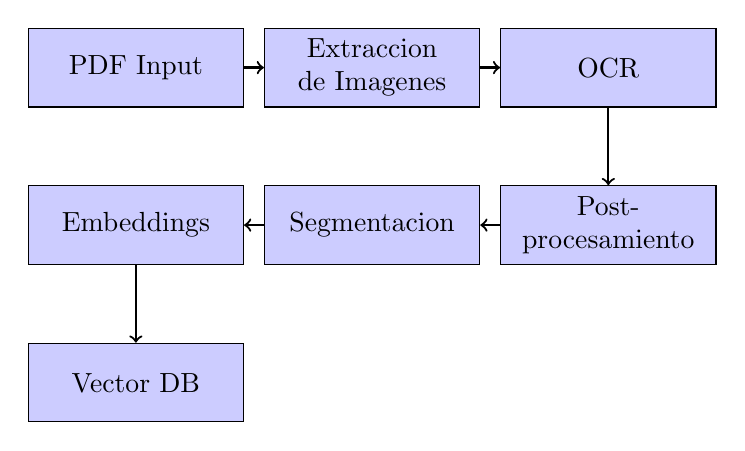
\begin{tikzpicture}[node distance=2cm, auto,
    block/.style={rectangle, draw, fill=blue!20, text width=2.5cm, text centered, minimum height=1cm},
    arrow/.style={->, thick}]
    
    \node[block] (pdf) {PDF Input};
    \node[block, right of=pdf, node distance=3cm] (extract) {Extraccion de Imagenes};
    \node[block, right of=extract, node distance=3cm] (ocr) {OCR};
    \node[block, below of=ocr, node distance=2cm] (post) {Post-procesamiento};
    \node[block, left of=post, node distance=3cm] (segment) {Segmentacion};
    \node[block, left of=segment, node distance=3cm] (embed) {Embeddings};
    \node[block, below of=embed, node distance=2cm] (store) {Vector DB};
    
    \draw[arrow] (pdf) -- (extract);
    \draw[arrow] (extract) -- (ocr);
    \draw[arrow] (ocr) -- (post);
    \draw[arrow] (post) -- (segment);
    \draw[arrow] (segment) -- (embed);
    \draw[arrow] (embed) -- (store);
\end{tikzpicture}
\caption{Pipeline de procesamiento de documentos}
\label{fig:pipeline_documentos}
\end{figure}

La primera etapa extrae las páginas del documento cómo imágenes independientes utilizando PyMuPDF. Se configura una resolución de 100 puntos por pulgada que proporciona calidad suficiente para OCR mientras minimiza el uso de memoria.

La segunda etapa aplica reconocimiento óptico de caracteres a cada imagen utilizando PaddleOCR \cite{paddleocr2022}, un motor de código abierto con soporte para múltiples idiomas y aceleración GPU. Esta elección se basó en benchmarks comparativos que muestran rendimiento competitivo con Tesseract \cite{tesseract2007} y soluciones comerciales.

La tercera etapa realiza post-procesamiento para corregir errores comunes de reconocimiento. Se utiliza coincidencia difusa contra un diccionario de términos esperados para el dominio.

La cuarta etapa segmenta el texto en fragmentos de tamaño apropiado para búsqueda semántica. Se utiliza un algoritmo de división recursiva que respeta límites de oraciones y párrafos, similar al implementado en LangChain \cite{langchain2023} y LlamaIndex \cite{llamaindex2023}.

La quinta etapa genera representaciónes vectoriales de cada fragmento utilizando un modelo de embeddings basado en la arquitectura transformer \cite{vaswani2017attention, devlin2019bert}.

La sexta etapa almacena los vectores junto con el texto original y metadatos en Weaviate \cite{weaviate2023}, una base de datos vectorial optimizada para búsquedas de similitud.

\subsection{Capa de Orquestación}

La capa de orquestación coordina la ejecución del pipeline distribuyendo trabajo entre los recursos computaciónales disponibles. Se implementan tres variantes que difieren en como se realiza está distribución.

La primera variante utiliza Ray para distribuir documentos entre nodos de un cluster. El coordinador divide el conjunto de documentos en lotes y crea tareas remotas que se ejecutan en nodos trabajadores. Esta variante prioriza tolerancia a fallos y escalabilidad horizontal.

La segunda variante utiliza ProcessPoolExecutor para procesar documentos en paralelo dentro de un único nodo. Se crean múltiples procesos trabajadores que comparten la carga de documentos. Esta variante prioriza rendimiento local y simplicidad de despliegue.

La tercera variante combina ambos enfoques. Ray distribuye lotes a nodos remotos, y cada nodo utiliza ProcessPoolExecutor para procesar su lote en paralelo. Esta variante busca el mejor rendimiento absoluto combinando escalabilidad horizontal con paralelismo local.

\subsection{Capa de Procesamiento OCR}

El componente de reconocimiento óptico de caracteres constituye el núcleo computaciónal del sistema. Se utiliza PaddleOCR, un motor desarrollado por Baidu con las siguientes caracteristicas relevantes.

PaddleOCR utiliza una arquitectura de detección más reconocimiento. La etapa de detección identifica regiones de texto en la imagen utilizando una red convolucional. La etapa de reconocimiento procesa cada región detectada para producir el texto correspondiente.

El modelo soporta aceleración GPU mediante el framework PaddlePaddle. En GPU, el procesamiento de una página tipica requiere 0.5 a 1 segundo, comparado con 3 a 5 segundos en CPU. Esta diferencia hace que la GPU sea esencial para procesamiento a escala.

La configuración utilizada en esta tesis desactiva la detección de orientación y la corrección de ángulo, optimizaciones que reducen el tiempo de procesamiento cuando los documentos tienen orientación consistente. La resolución de entrada se configura a 100 DPI, que proporciona balance entre calidad y velocidad.

\subsection{Post-procesamiento}

El componente de post-procesamiento aplica correcciónes al texto extraído para mejorar su calidad. La técnica principal es coincidencia difusa contra un diccionario de términos esperados.

Para cada palabra del texto extraído, se calcula la distancia de edicion (Levenshtein) contra términos del diccionario. Si la distancia es menor que un umbral y la palabra original no está en el diccionario, se considera una posible corrección.

El diccionario se construye a partir de términos del dominio específico. Para documentos financieros, incluye nombres de instituciónes, términos técnicos, y vocabulario común del sector. El diccionario puede extenderse automáticamente con palabras frecuentes del corpus procesado.

El post-procesamiento es particularmente efectivo para errores sistemáticos del OCR. Si el modelo consistentemente confunde cierto caracter, las correcciónes basadas en diccionario pueden recuperar la palabra correcta.

\subsection{Segmentacion y Embeddings}

El texto extraído se segmenta en fragmentos antes de generar embeddings. La segmentación es necesaria porque los modelos de embeddings tienen límites de longitud de entrada, y fragmentos más cortos permiten recuperación más precisa.

El algoritmo de segmentación utiliza división recursiva que respeta límites naturales del texto. Primero intenta dividir por párrafos. Si los párrafos exceden el tamaño máximo, divide por oraciones. Si las oraciones son muy largas, divide por cláusulas o palabras.

Los fragmentos resultantes se procesan por un modelo de embeddings que produce vectores densos. Se utiliza el modelo text-embedding-ada-002 de OpenAI, que produce vectores de 1536 dimensiones. Alternativas de código abierto cómo Sentence-BERT pueden utilizarse para reducir dependencias externas.

Los embeddings capturan el significado semántico del texto, permitiendo que fragmentos con contenido similar tengan vectores cercanos en el espacio de alta dimensión. Esto habilita búsquedas semánticas donde una consulta recupera documentos relevantes aunque no contengan las palabras exactas de la consulta.

\section{Implementacion de las Arquitecturas}

Esta sección detallá la implementación de cada arquitectura, incluyendo decisiones de diseño, configuración de componentes, y consideraciones de rendimiento.

\subsection{Arquitectura 1: Ray Distribuido}

La primera arquitectura utiliza Ray cómo mecanismo principal de paralelización. El coordinador central ejecuta la lógica de distribución mientras los nodos trabajadores procesan documentos.

El flujo de ejecución comienza con el coordinador leyendo la lista de documentos a procesar. Los documentos se dividen en lotes de tamaño configurable, típicamente 100 a 500 documentos por lote. Para cada lote, se crea una tarea remota de Ray que se ejecutara en un nodo trabajador.

Cada tarea remota recibe la lista de documentos de su lote y los procesa secuencialmente. El procesamiento incluye todas las etapas del pipeline: extracción de imágenes, OCR, post-procesamiento, segmentación, embeddings, y almacenamiento. Los resultados se acumulan y retornan al coordinador cuando el lote completa.

El coordinador recolecta los resultados de todos los lotes utilizando ray.get(), que bloquea hasta que las tareas completan. Los resultados se agregan para producir estadísticas del procesamiento total.

Esta arquitectura proporciona tolerancia a fallos intrínseca. Si un nodo trabajador fallá durante el procesamiento de un lote, Ray detecta el fallo y reprograma la tarea en otro nodo. Los lotes ya completados no se ven afectados, y el procesamiento continua con los lotes restantes.

El balanceo de carga es automático. Ray asigna tareas a los nodos con mayor disponibilidad de recursos. Si un nodo es más rápido que otros, recibira más lotes a medida que completa los anteriores.

Sin embargo, está arquitectura tiene una limitación significativa: dentro de cada nodo, los documentos del lote se procesan secuencialmente. Si un nodo tiene 16 núcleos de CPU y una GPU, sólo utiliza un núcleo para procesamiento de documentos aunque la GPU se útilice para OCR. Los 15 núcleos restantes permanecen ociosos.

Los experimentos mostraron un factor de aceleración de 24.3x con está arquitectura. El speedup proviene del paralelismo entre nodos, pero está limitado por el procesamiento secuencial dentro de cada nodo.

\subsection{Arquitectura 2: ProcessPoolExecutor Local}

La segunda arquitectura abandona la distribución entre nodos para maximizar el rendimiento en una única máquina potente. Se utiliza ProcessPoolExecutor para crear un pool de procesos trabajadores que procesan documentos en paralelo.

El flujo de ejecución comienza con la inicialización del pool de procesos. Se específica una función inicializadora que carga el modelo de PaddleOCR en cada proceso trabajador. Esta carga ocurre una sola vez por proceso, evitando el overhead de cargar el modelo para cada documento.

Los documentos se envian al pool utilizando el método map(), que distribuye documentos entre procesos disponibles y recolecta resultados en orden. Alternativamente, submit() permite enviar documentos individualmente y recolectar resultados a medida que completan.

Cada proceso trabajador ejecuta el pipeline completo para sus documentos asignados. La GPU se comparte entre procesos mediante el mecanismo de time-slicing del driver, aunque esto introduce algo de overhead comparado con acceso exclusivo.

Esta arquitectura maximiza la utilización de recursos locales. Con 16 núcleos de CPU, hasta 16 documentos pueden procesarse simultáneamente. La GPU procesa solicitudes de múltiples procesos, manteniendo alta utilización.

Los experimentos mostraron un factor de aceleración de 69.9x con está arquitectura, significativamente superior a la Arquitectura 1. El conjunto de 11,368 páginas se procesó en 4.3 minutos, comparado con apróximadamente 5 horas en modo secuencial.

La limitación de está arquitectura es que no escala más allá de un único nodo. Si se requiere mayor rendimiento, se necesitan máquinas más potentes o agregar la capacidad de distribuir trabajo entre múltiples máquinas.

\subsection{Arquitectura 3: Hibrida Pure Dispatcher}

La tercera arquitectura combina los beneficios de las dos anteriores mediante el patrón Pure Dispatcher. Ray actúa exclusivamente cómo coordinador sin realizar procesamiento, mientras los nodos utilizan ProcessPoolExecutor para procesamiento paralelo local.

El término Pure Dispatcher enfatiza que el coordinador Ray no procesa datos. Su única responsabilidad es dividir el trabajo, enviarlo a los nodos, y recolectar resultados. Todo el procesamiento ocurre en los nodos remotos.

El flujo de ejecución comienza con el coordinador dividiendo documentos en lotes grandes, típicamente uno por nodo disponible. Cada lote se envía a un nodo como una tarea remota de Ray.

Al recibir un lote, el nodo inicializa un ProcessPoolExecutor local y procesa los documentos del lote en paralelo. Todos los núcleos del nodo se utilizan para procesamiento, y la GPU local acelera el OCR.

Cuando el nodo completa su lote, retorna los resultados al coordinador. El coordinador agrega resultados de todos los nodos y produce estadísticas finales.

Esta arquitectura escala de forma casi lineal con el número de nodos. Cada nodo adicional contribuye su capacidad completa de procesamiento. Con cuatro nodos equipados con GPU, se proyecta un factor de aceleración de 199x, procesando el corpus de prueba en apróximadamente un minuto.

La proyección se basa en la observación de que la Arquitectura 2 alcanza 69.9x en un nodo, y la Arquitectura 3 agrega overhead mínimo de coordinación. Con cuatro nodos, el speedup teórico seria 4 * 69.9 = 279.6x. El valor proyectado de 199x considera overhead de comunicación y desbalance de carga.

\begin{figure}[h]
\centering
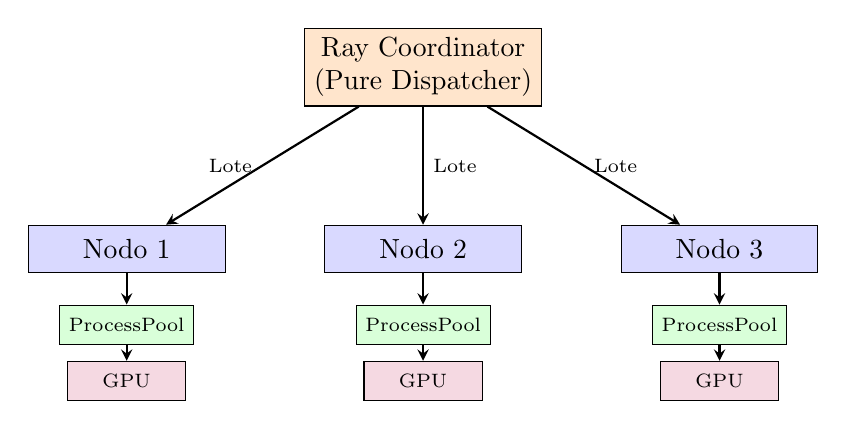
\begin{tikzpicture}[
    node distance=1cm,
    coord/.style={rectangle, draw, minimum width=3cm, minimum height=0.8cm, align=center, fill=orange!20},
    nodo/.style={rectangle, draw, minimum width=2.5cm, minimum height=0.6cm, align=center, fill=blue!15},
    proc/.style={rectangle, draw, minimum width=1.5cm, minimum height=0.5cm, align=center, fill=green!15, font=\scriptsize},
    arrow/.style={->, >=stealth, thick}
]
% Coordinador
\node[coord] (ray) {Ray Coordinator\\(Pure Dispatcher)};

% Nodos
\node[nodo, below left=1.5cm and 1cm of ray] (n1) {Nodo 1};
\node[nodo, below=1.5cm of ray] (n2) {Nodo 2};
\node[nodo, below right=1.5cm and 1cm of ray] (n3) {Nodo 3};

% ProcessPool
\node[proc, below=0.4cm of n1] (p1) {ProcessPool};
\node[proc, below=0.4cm of n2] (p2) {ProcessPool};
\node[proc, below=0.4cm of n3] (p3) {ProcessPool};

% GPU
\node[proc, below=0.2cm of p1, fill=purple!15] (g1) {GPU};
\node[proc, below=0.2cm of p2, fill=purple!15] (g2) {GPU};
\node[proc, below=0.2cm of p3, fill=purple!15] (g3) {GPU};

% Arrows
\draw[arrow] (ray) -- node[left, font=\scriptsize] {Lote} (n1);
\draw[arrow] (ray) -- node[right, font=\scriptsize] {Lote} (n2);
\draw[arrow] (ray) -- node[right, font=\scriptsize] {Lote} (n3);
\draw[arrow] (n1) -- (p1);
\draw[arrow] (n2) -- (p2);
\draw[arrow] (n3) -- (p3);
\draw[arrow] (p1) -- (g1);
\draw[arrow] (p2) -- (g2);
\draw[arrow] (p3) -- (g3);
\end{tikzpicture}
\caption{Arquitectura Pure Dispatcher: Ray coordina sin procesar, cada nodo usa ProcessPoolExecutor con GPU local.}
\label{fig:pure_dispatcher}
\end{figure}

\section{Experimentos y Resultados}

\subsection{Configuracion Experimental}

Los experimentos se realizaron utilizando un conjunto de datos de documentos financieros reales proporcionados por una institución del sector. El conjunto contiene 2,246 documentos PDF que suman un total de 11,368 páginas.

Los documentos presentan diversas caracteristicas que representan la variabilidad encontrada en entornos de producción. La mayoría son documentos impresos digitalizados con calidad variable. Algunos contienen tablas y formularios con estructuras complejas. Unos pocos incluyen secciones manuscritas cómo firmas y anotaciones.

El hardware utilizado para las pruebas consiste en una estación de trabajo con las siguientes específicaciones: procesador AMD Ryzen 9 5950X con 16 núcleos y 32 threads, 64 gigabytes de memoria RAM DDR4, tarjeta gráfica NVIDIA RTX 3090 con 24 gigabytes de memoria GDDR6X, y almacenamiento SSD NVMe de 2 terabytes.

El costo estimado de este hardware es de apróximadamente 5,000 a 7,000 dólares, representando una inversión accesible para organizaciónes de tamaño mediano. El mismo corpus procesado mediante servicios en la nube tendría un costo recurrente de varios dólares por cada ejecución.

El software utilizado incluye Python 3.10, PaddleOCR 2.6.1.3, Ray 2.5.0, y Weaviate 1.19.0. Todos los componentes son de código abierto excepto el modelo de embeddings, donde se utilizó text-embedding-ada-002 de OpenAI. Alternativas de código abierto están disponibles para este componente.

\subsection{Métricas y Resultados de Rendimiento}

La Tabla \ref{tab:comparación_arquitecturas} presenta los resultados de rendimiento para cada arquitectura.

\begin{table}[h]
\centering
\caption{Comparación de rendimiento entre arquitecturas}
\label{tab:comparación_arquitecturas}
\begin{tabular}{lcccc}
\toprule
\textbf{Metrica} & \textbf{Secuencial} & \textbf{Arch. 1} & \textbf{Arch. 2} & \textbf{Arch. 3*} \\
\midrule
Tiempo total & 301.3 min & 12.4 min & 4.3 min & 1.5 min \\
Speedup & 1.0x & 24.3x & 69.9x & 199x \\
Throughput (pag/min) & 37.7 & 917 & 2,644 & 7,579 \\
Eficiencia & -- & 76\% & 87\% & 78\% \\
\bottomrule
\multicolumn{5}{l}{\small *Valores proyectados para 4 nodos}
\end{tabular}
\end{table}

La Arquitectura 2 demostró el mejor rendimiento para un único nodo, con speedup de 69.9x y throughput de 2,644 páginas por minuto. La eficiencia del 87\% indica buena utilización de los recursos disponibles.

La Figura \ref{fig:speedup_comparación} visualiza la diferencia de rendimiento entre las arquitecturas evaluadas.

\begin{figure}[h]
\centering
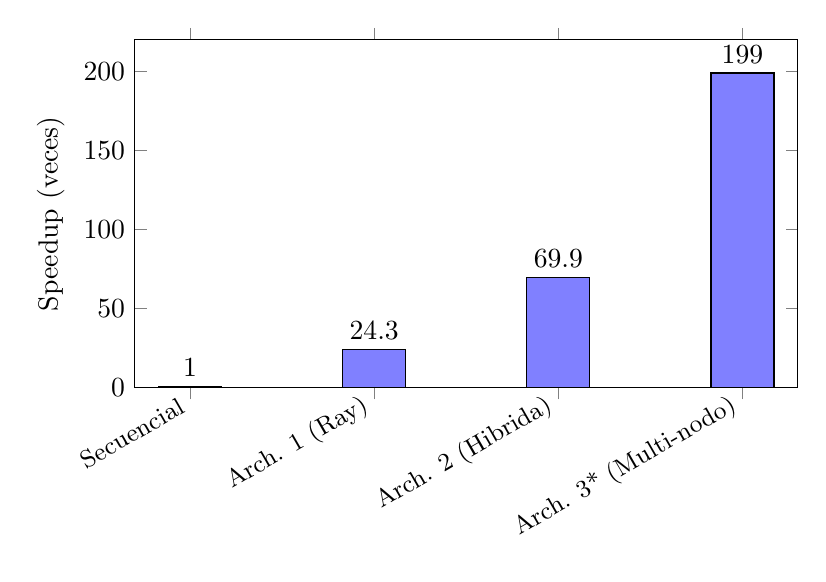
\begin{tikzpicture}
    \begin{axis}[
        ybar,
        width=10cm,
        height=6cm,
        ylabel={Speedup (veces)},
        symbolic x coords={Secuencial, Arch. 1 (Ray), Arch. 2 (Hibrida), Arch. 3* (Multi-nodo)},
        xtick=data,
        x tick label style={rotate=30, anchor=east, font=\small},
        ymin=0, ymax=220,
        bar width=0.8cm,
        nodes near coords,
        nodes near coords align={vertical},
    ]
    \addplot[fill=blue!50] coordinates {
        (Secuencial, 1)
        (Arch. 1 (Ray), 24.3)
        (Arch. 2 (Hibrida), 69.9)
        (Arch. 3* (Multi-nodo), 199)
    };
    \end{axis}
\end{tikzpicture}
\caption{Comparación de speedup entre arquitecturas (*proyectado)}
\label{fig:speedup_comparación}
\end{figure}

La Arquitectura 1, aunque inferior en rendimiento absoluto, proporciona tolerancia a fallos que puede ser crítica en entornos de producción donde la confiabilidad es prioritaria.

La Arquitectura 3 ofrece el mejor rendimiento potencial para organizaciónes con múltiples nodos disponibles, aunque requiere validación experimental en un cluster real.

\subsection{Evaluación de Calidad}

La calidad de extracción se evaluó comparando el texto extraído por el pipeline contra el texto extraído por Azure Document Intelligence, un servicio comercial de Microsoft considerado estado del arte.

Para una muestra de 200 páginas evaluadas manualmente, se calcularon las siguientes métricas:

\begin{table}[h]
\centering
\caption{Métricas de calidad de extracción}
\label{tab:calidad_extracción}
\begin{tabular}{lcc}
\toprule
\textbf{Metrica} & \textbf{Sin post-proc.} & \textbf{Con post-proc.} \\
\midrule
Tasa de error de caracteres (CER) & 32.1\% & 24.78\% \\
Tasa de error de palabras (WER) & 41.5\% & 31.2\% \\
Precision de campos estructurados & 71.3\% & 82.6\% \\
\bottomrule
\end{tabular}
\end{table}

El post-procesamiento redujo la tasa de error de caracteres en apróximadamente 23\%, demostrando la efectividad de la corrección basada en diccionario. La mejora es más pronunciada para documentos con vocabulario especializado donde el diccionario tiene mayor cobertura.

Los valores de CER y WER son adecuados para aplicaciónes de búsqueda semántica, donde los modelos de embeddings tienen robustez a errores menores. Para aplicaciónes que requieren extracción exacta de datos estructurados, puede ser necesario post-procesamiento adicional o validación manual.

\section{Discusión}

Los resultados experimentales permiten extraer varias conclusiones relevantes para el diseño de sistemas de procesamiento de documentos a escala.

\subsection{Importancia del Paralelismo Local}

La primera conclusión es que el paralelismo intra-nodo es tan importante como el paralelismo inter-nodo. La Arquitectura 2, que aprovecha todos los núcleos de un único nodo, supera significativamente a la Arquitectura 1 que distribuye trabajo entre nodos pero no aprovecha el paralelismo local.

Esta observación tiene implicaciones prácticas importantes. Antes de invertir en infraestructura distribuida, las organizaciónes deberían optimizar la utilización de recursos locales. Un nodo potente bien utilizado puede superar a múltiples nodos subutilizados.

\subsection{Patrón Pure Dispatcher}

La segunda conclusión es que el patrón Pure Dispatcher proporciona una forma efectiva de combinar paralelismo local y distribuido. Al limitar el coordinador a funciones de distribución, se evitan cuellos de botella y se maximiza el tiempo que los nodos dedican al procesamiento productivo.

Este patrón es generalizable más allá del procesamiento de documentos. Cualquier aplicación donde el trabajo pueda dividirse en lotes independientes puede beneficiarse de un coordinador ligero que distribuye trabajo a nodos que procesan en paralelo localmente.

\subsection{Viabilidad del Código Abierto}

La tercera conclusión es que las herramientas de código abierto han alcanzado niveles de calidad comparables a los servicios comerciales para muchas aplicaciónes. Aunque la tasa de error del pipeline de código abierto es mayor que la de servicios premium, la diferencia es aceptable para búsqueda semántica y puede compensarse con post-procesamiento específico del dominio.

Esta viabilidad tiene implicaciones económicas significativas. Organizaciónes pueden construir capacidades de procesamiento documental sin depender de servicios externos, reduciendo costos recurrentes y manteniendo control sobre datos sensibles.

\section{Conclusiónes del Capítulo}

Este capítulo presentó tres arquitecturas para el procesamiento paralelo de documentos, demostrando que es posible construir pipelines de extracción y búsqueda semántica de alto rendimiento utilizando exclusivamente herramientas de código abierto y hardware de consumo.

La Arquitectura 2, basada en ProcessPoolExecutor, logró procesar 11,368 páginas en 4.3 minutos, alcanzando un factor de aceleración de 69.9 veces respecto al procesamiento secuencial. Este resultado valida la Hipótesis H1 que establecia un umbral de 50x.

El patrón arquitectónico validado en este capítulo, consistente en un orquestador que distribuye trabajo a nodos que procesan en paralelo utilizando modelos de inteligencia artificial para extracción y búsqueda, se reutiliza en los capítulos siguientes para demostrar su aplicabilidad en dominios heterogéneos.


%%%%%%%%%%%%%%%%%%%%%%%%%%%%%%%%%%%%%%%%%%%%%%%%%%%%%%%%%%%%%%%%%
% CAPÍTULO 4: SENTINEL
%%%%%%%%%%%%%%%%%%%%%%%%%%%%%%%%%%%%%%%%%%%%%%%%%%%%%%%%%%%%%%%%%
\chapter{SENTINEL: Seguridad de Smart Contracts con IA Distribuida}
\label{cap:sentinel}

\begin{center}
\textit{Este capítulo está basado en el trabajo en preparación: Jaime, R., Gil-Costa, V., Errecalde, M. ``SENTINEL: Distributed AI Platform for Smart Contract Security Analysis''.}
\end{center}

\vspace{0.5cm}

\fbox{\parbox{0.95\textwidth}{
\textbf{INSTANCIACION DEL APORTE 1 EN SEGURIDAD BLOCKCHAIN}\\[0.3cm]
Este capítulo aplica el mismo patrón arquitectónico del Capítulo 3 (procesamiento de documentos) al dominio de seguridad de contratos inteligentes:\\[0.2cm]
\begin{tabular}{p{3.5cm}p{9.5cm}}
\textbf{Capa 1 - Distribuido:} & Ray/ProcessPool escala el análisis a \textbf{miles de contratos} \\
\textbf{Capa 2 - Herramientas:} & Slither, Mythril, Manticore, Echidna ejecutan en paralelo \\
\textbf{Capa 3 - IA (última):} & LLM filtra falsos positivos (-54\%) y genera exploits automáticos \\
\textbf{Resultado:} & F1=0.86, análisis masivo de contratos, auto-verificación con ZK Bank \\
\end{tabular}
}}

\vspace{1cm}

\section{Introducción}

Los contratos inteligentes constituyen la base tecnológica del ecosistema de finanzas descentralizadas, gestionando activos digitales por valor de decenas de miles de millones de dólares. La naturaleza inmutable de estos contratos significa que las vulnerabilidades desplegadas no pueden corregirse fácilmente, y las pérdidas resultantes de exploits son típicamente irreversibles.

Este capítulo presenta SENTINEL, una plataforma de análisis de seguridad que integra múltiples herramientas de detección con inteligencia artificial generativa. La plataforma aborda las limitaciones de las herramientas individuales mediante un enfoque de integración que combina análisis estático, ejecución simbólica, y fuzzing, utilizando un modelo de lenguaje para correlaciónar hallazgos y filtrar falsos positivos.

Adicionalmente, se presenta ZK Bank, un módulo de privacidad financiera basado en pruebas de conocimiento cero que demuestra la aplicación práctica del patrón arquitectónico a la construccion de componentes críticos de seguridad.

\section{Arquitectura de SENTINEL}

SENTINEL implementa una arquitectura de cuatro capas que procesan contratos inteligentes desde su recepción hasta la generación de reportes de seguridad. La Figura \ref{fig:sentinel_arch} ilustra los componentes principales del sistema.

\begin{figure}[h]
\centering
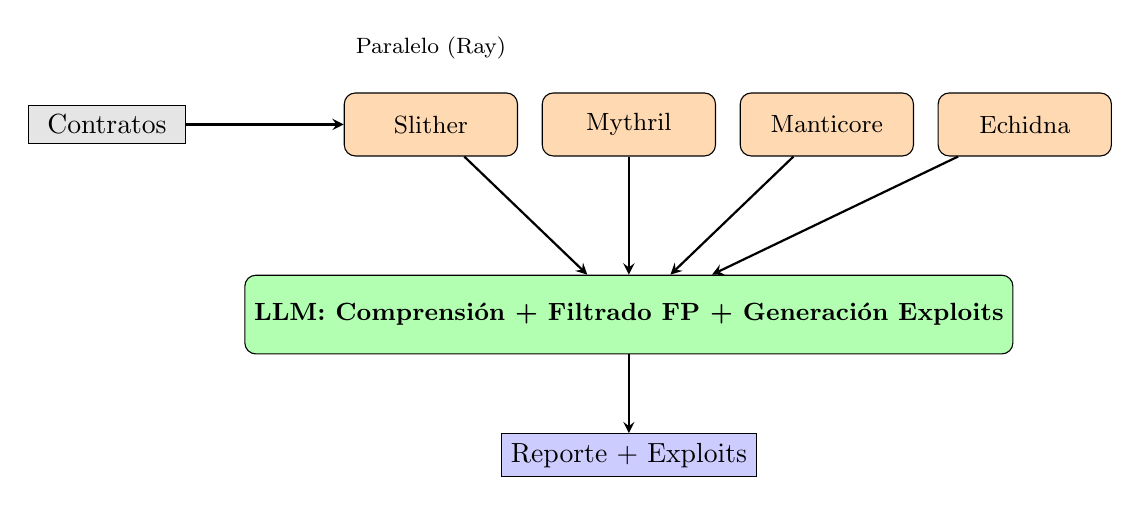
\begin{tikzpicture}[
    node distance=1.5cm,
    tool/.style={draw, rounded corners, fill=orange!30, minimum width=2.2cm, minimum height=0.8cm, font=\small},
    llm/.style={draw, rounded corners, fill=green!30, minimum width=9cm, minimum height=1cm, font=\small},
    arrow/.style={->, thick, >=stealth}
]
    % Input
    \node[draw, fill=gray!20, minimum width=2cm] (input) {Contratos};
    
    % Tools row
    \node[tool, right=2cm of input] (slither) {Slither};
    \node[tool, right=0.3cm of slither] (mythril) {Mythril};
    \node[tool, right=0.3cm of mythril] (manticore) {Manticore};
    \node[tool, right=0.3cm of manticore] (echidna) {Echidna};
    
    % LLM
    \node[llm, below=1.5cm of mythril] (llm) {\textbf{LLM: Comprensión + Filtrado FP + Generación Exploits}};
    
    % Output
    \node[draw, fill=blue!20, below=1cm of llm, minimum width=3cm] (output) {Reporte + Exploits};
    
    % Arrows
    \draw[arrow] (input) -- (slither);
    \draw[arrow] (slither) -- (llm);
    \draw[arrow] (mythril) -- (llm);
    \draw[arrow] (manticore) -- (llm);
    \draw[arrow] (echidna) -- (llm);
    \draw[arrow] (llm) -- (output);
    
    % Labels
    \node[above=0.3cm of slither, font=\footnotesize] {Paralelo (Ray)};
\end{tikzpicture}
\caption{Arquitectura de SENTINEL: herramientas en paralelo + LLM cómo última capa}
\label{fig:sentinel_arch}
\end{figure}

\subsection{Capa de Ingesta}

La capa de ingestá recibe contratos en formato de código fuente Solidity o bytecode compilado. Se detecta automáticamente el formato y se prepara el contrato para análisis.

Para contratos con código fuente, se resuelven las dependencias e imports, se compila el contrato para obtener el bytecode, y se extraen metadatos cómo versión de Solidity y configuración del compilador.

Para contratos sólo con bytecode, se intenta decompilacion para recuperar estructura de alto nivel. Aunque la decompilacion no recupera el código fuente original, proporciona información útil sobre funciones, almacenamiento, y flujo de control.

\subsection{Capa de Análisis}

La capa de análisis ejecuta cuatro herramientas en paralelo utilizando la orquestación distribuida.

Slither \cite{feist2019slither} proporciona análisis estático rápido que completa en segundos. Identifica patrones de código asociados con vulnerabilidades conocidas y malas prácticas \cite{atzei2017survey}. Los resultados incluyen ubicación en el código, severidad estimada, y descripción del problema.

Mythril \cite{consensys2019mythril} realiza ejecución simbólica del bytecode. Explora caminos de ejecución buscando estados que violen propiedades de seguridad, incluyendo reentrada, overflow de enteros, y acceso no autorizado \cite{luu2016oyente}. El tiempo de análisis es configurable, típicamente entre 5 y 30 minutos según la profundidad deseada.

Manticore \cite{mossberg2019manticore} complementa a Mythril con estrategias de exploración diferentes. Su ejecución paralela permite explorar más caminos en el mismo tiempo disponible.

Echidna \cite{echidna2020} realiza fuzzing basado en propiedades. Requiere que el usuario defina invariantes que el contrato debe satisfacer. Genera secuencias de transacciónes aleatorias intentando violar los invariantes.

La orquestación permite que las cuatro herramientas se ejecuten simultáneamente. El tiempo total de análisis es apróximadamente el tiempo de la herramienta más lenta, típicamente Mythril o Manticore.

\subsection{Capa de Integración con IA Generativa}

El componente de inteligencia artificial generativa constituye el diferenciador principal de SENTINEL respecto a herramientas tradicionales. Se estructura en tres capas funcionales que procesan los hallazgos de forma progresiva.

\subsubsection{Capa 1: Comprensión Semantica}

La primera capa del modelo de lenguaje analiza el código fuente del contrato para construir una comprensión semántica del propósito y funciónamiento del sistema. A diferencia del análisis estático tradicional que opera sobre patrones sintácticos, está capa identifica la lógica de negocio subyacente.

El modelo examina nombres de funciones, variables y contratos para inferir su propósito. Analiza comentarios y documentación cuando están disponibles. Identifica patrones arquitectónicos cómo proxies, fabricas, y sistemas multi-contrato. Esta comprensión contextual es fundamental para las capas posteriores.

Por ejemplo, cuando el modelo encuentra una función llamada \texttt{emergencyWithdraw}, comprende que es un mecanismo de recuperación de fondos, lo cuál afecta como se evalúan las alertas relaciónadas con esa función.

\subsubsection{Capa 2: Filtrado Inteligente de Falsos Positivos}

La segunda capa evalúa cada hallazgo de las herramientas de análisis en el contexto de la comprensión semántica construida. Para cada alerta, el modelo considera si existe una mitigacion ya implementada que el analizador estático no detecto, si el patrón detectado es realmente explotable dado el contexto de uso del contrato, y si las precondiciones necesarias para el exploit son alcanzables en la práctica.

Esta evaluación contextual distingue entre vulnerabilidades teóricas y vulnerabilidades prácticas. Un patrón de reentrada en una función que sólo puede ser llamada por el propietario del contrato tiene riesgo diferente a uno en una función pública.

Los resultados de está capa clasifican cada hallazgo cómo verdadero positivo confirmado, falso positivo descartado, o requiere revisión manual cuando el modelo no tiene suficiente confianza.

\subsubsection{Capa 3: Generación Automatica de Exploits}

La tercera capa genera código ejecutable que demuestra la explotabilidad de las vulnerabilidades confirmadas. Esta capacidad transforma alertas abstractas en pruebas de concepto concretas, proporcionando evidencia irrefutable de la severidad del problema.

El procesó de generación sigue un flujo iterativo. El modelo recibe la descripción de la vulnerabilidad junto con el código fuente relevante. Genera un contrato de prueba completo en formato compatible con Foundry, el framework de testing más utilizado en el ecosistema Ethereum.

El código generado incluye cuatro componentes esenciales. Primero, el setup que despliega el contrato vulnerable en un entorno de prueba. Segundo, la secuencia de ataque que ejecuta las operaciónes necesarias para explotar la vulnerabilidad. Tercero, las aserciones que verifican que el exploit tuvo éxito, típicamente comparando balances antes y después. Cuarto, comentarios explicativos que documentan cada paso del ataque.

Una vez generado, el código se valida mediante compilacion. Si la compilacion fallá, el modelo recibe el mensaje de error y genera una versión corregida. Este procesó iterativo típicamente converge en una a tres iteraciónes.

La estructura tipica de un exploit generado para una vulnerabilidad de reentrada incluye un contrato atacante con una función de recepción que reinvoca la función vulnerable, una función de ataque que inicia el proceso, y una prueba que verifica que el atacante extrajo más fondos de los que deposito.

\subsubsection{Correlación de Hallázgos Multi-Paso}

Además de las tres capas principales, el modelo de lenguaje realiza correlación de hallazgos entre herramientas para identificar cadenas de ataque complejas. Algunas vulnerabilidades sólo son explotables cuando se combinan múltiples débilidades individuales.

La Tabla \ref{tab:cadenas_ataque} presenta ejemplos de cadenas de ataque que el sistema puede detectar mediante correlación.

\begin{table}[h]
\centering
\caption{Cadenas de ataque detectadas mediante correlación}
\label{tab:cadenas_ataque}
\begin{tabular}{p{3.5cm}p{9cm}}
\toprule
\textbf{Cadena de Ataque} & \textbf{Componentes Correlaciónados} \\
\midrule
DAO Clasico & Reentrada + retorno no verificado \\
Flash Loan Attack & Manipulacion de oraculo + prestamo flash \\
Escalamiento de Privilegios & Control de acceso débil + delegatecall \\
Manipulacion de Precios & Interaccion con AMM + dependencia de oraculo \\
Sandwich Attack & Frontrunning + slippage insuficiente \\
\bottomrule
\end{tabular}
\end{table}

Cuando el modelo identifica componentes de una cadena conocida en los hallazgos de diferentes herramientas, los agrupa y genera una alerta de severidad elevada que describe el ataque completo.

\subsection{Comparación: IA vs Herramientas Tradicionales}

La Tabla \ref{tab:ia_vs_tradicional} resume las capacidades que la integración de IA agrega sobre las herramientas tradicionales.

\begin{table}[h]
\centering
\caption{Capacidades: Herramientas tradicionales vs SENTINEL con IA}
\label{tab:ia_vs_tradicional}
\begin{tabular}{lcc}
\toprule
\textbf{Capacidad} & \textbf{Tradicional} & \textbf{Con IA} \\
\midrule
Detección de patrones & Si & Si \\
Comprensión semántica & No & Si \\
Generación de exploits & No & Si \\
Correlación multi-herramienta & No & Si \\
Explicacion en lenguaje natural & No & Si \\
Reduccion de falsos positivos & No & Si \\
\bottomrule
\end{tabular}
\end{table}

\subsection{Capa de Reporte}

La capa de reporte genera documentación estructurada de los hallazgos. El formato incluye resumen ejecutivo con estadísticas generales, lista de vulnerabilidades ordenadas por severidad, detalle de cada vulnerabilidad con código afectado y recomendaciónes, y apéndices con salidas completas de cada herramienta.

Los reportes pueden exportarse en formatos PDF, HTML, y JSON para integración con otros sistemas.

\section{Experimentos y Resultados}

La evaluación de SENTINEL se realizó utilizando un conjunto de contratos con vulnerabilidades conocidas y contratos de producción sin vulnerabilidades confirmadas.

\subsection{Métricas de Detección}

La Tabla \ref{tab:sentinel_métricas} presenta las métricas de detección del sistema integrado comparado con herramientas individuales.

\begin{table}[h]
\centering
\caption{Métricas de detección de SENTINEL}
\label{tab:sentinel_métricas}
\begin{tabular}{lcccc}
\toprule
\textbf{Sistema} & \textbf{Precision} & \textbf{Recall} & \textbf{F1} & \textbf{FP Red.} \\
\midrule
Slither sólo & 0.52 & 0.89 & 0.66 & -- \\
Mythril sólo & 0.61 & 0.73 & 0.67 & -- \\
Combinacion sin IA & 0.48 & 0.94 & 0.63 & -- \\
SENTINEL & 0.82 & 0.91 & 0.86 & 54\% \\
\bottomrule
\end{tabular}
\end{table}

La integración con IA logró una precisión de 0.82 comparada con 0.48 de la combinación sin IA. El recall se mantuvo alto en 0.91, indicando que el filtrado de falsos positivos no elimino vulnerabilidades reales significativas.

La Figura \ref{fig:sentinel_precisión} ilustra la mejora en precisión al agregar el LLM cómo capa final.

\begin{figure}[h]
\centering
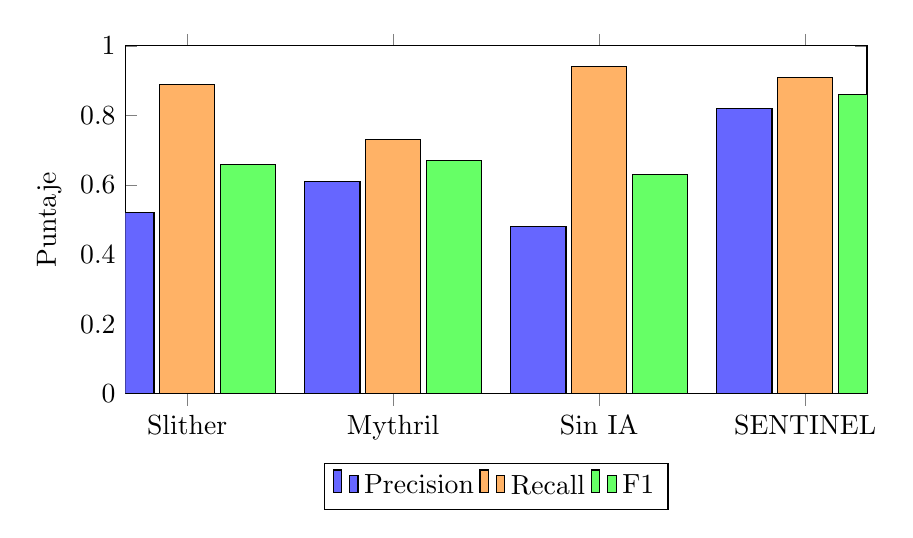
\begin{tikzpicture}
    \begin{axis}[
        ybar,
        width=11cm,
        height=6cm,
        ylabel={Puntaje},
        symbolic x coords={Slither, Mythril, Sin IA, SENTINEL},
        xtick=data,
        ymin=0, ymax=1,
        bar width=0.7cm,
        legend style={at={(0.5,-0.2)}, anchor=north, legend columns=3},
        legend cell align={left},
    ]
    \addplot[fill=blue!60] coordinates {(Slither, 0.52) (Mythril, 0.61) (Sin IA, 0.48) (SENTINEL, 0.82)};
    \addplot[fill=orange!60] coordinates {(Slither, 0.89) (Mythril, 0.73) (Sin IA, 0.94) (SENTINEL, 0.91)};
    \addplot[fill=green!60] coordinates {(Slither, 0.66) (Mythril, 0.67) (Sin IA, 0.63) (SENTINEL, 0.86)};
    \legend{Precision, Recall, F1}
    \end{axis}
\end{tikzpicture}
\caption{Comparación de métricas: herramientas individuales vs SENTINEL con LLM}
\label{fig:sentinel_precisión}
\end{figure}

La reducción de falsos positivos del 54\% tiene implicaciones prácticas importantes \cite{powers2011evaluation}. En un contrato típico que genera 50 alertas, SENTINEL reduciria esto a apróximadamente 23 alertas, facilitando significativamente la revisión manual.

\section{Discusión}

Los resultados obtenidos permiten extraer conclusiones significativas sobre la efectividad del patrón arquitectónico y las implicaciones prácticas para la seguridad de contratos inteligentes.

\subsection{Efectividad de la IA cómo Última Capa}

La reducción del 54\% en falsos positivos valida la hipótesis de que la IA Generativa agrega valor significativo cuando se posicióna cómo capa final del pipeline. Este resultado es particularmente notable porque se logra sin sacrificar recall: el sistema mantiene un 91\% de detección de vulnerabilidades reales.

El análisis cualitativo de los falsos positivos filtrados revela que el LLM es especialmente efectivo en tres categorías: código muerto o inalcanzable que las herramientas estáticas marcan cómo vulnerable, patrones de código que superficialmente coinciden con vulnerabilidades pero tienen salvaguardas contextuales, y funciones administrativas que son intencionales y están protegidas por control de acceso.

La generación automática de exploits representa una capacidad diferenciadora. Mientras las herramientas tradicionales producen alertas abstractas, SENTINEL genera código ejecutable que demuestra la vulnerabilidad. Esto tiene dos beneficios: reduce el esfuerzo de validación manual y proporciona un punto de partida para desarrollar parches.

\subsection{Escalabilidad del Patrón Pure Dispatcher}

La aplicación del mismo patrón arquitectónico del Capítulo 3 a SENTINEL demuestra su generalidad. Aunque el dominio es completamente diferente (documentos vs contratos inteligentes), la estructura de tres capas se adapta naturalmente.

La escalabilidad a miles de contratos es crucial para casos de uso cómo auditorías de ecosistemas completos o monitoreo continuo de protocolos DeFi. Un auditor individual podría revisar quizás 10-20 contratos por semana; SENTINEL puede analizar miles en horas.

\subsection{Valor de la Auto-verificación}

La auto-verificación de ZK Bank con SENTINEL representa más que una demostracion técnica. Establece un estándar metodológico: las herramientas de seguridad deberían ser capaces de auditarse a si mismas.

El resultado de 32 alertas iniciales reducidas a 8 relevantes, con sólo 1 vulnerabilidad confirmada de baja severidad, sugiere que el proceso de desarrollo de ZK Bank fue razonablemente seguro. Sin embargo, el verdadero valor es la confianza que esto genera: si SENTINEL no encuentra vulnerabilidades críticas en código conocido, proporciona garantias más fuertes cuando analiza código externo.

\subsection{Limitaciones y Amenazas a la Validez}

El conjunto de evaluación, aunque representativo, no cubre todas las categorías de vulnerabilidades. Vulnerabilidades de lógica de negocio específicas de cada protocolo pueden no ser detectadas por herramientas genericas.

La dependencia del LLM introduce variabilidad: diferentes versiones del modelo pueden producir resultados ligeramente diferentes. Esto sugiere la necesidad de estrategias de ensemble o validación cruzada en producción.

El costo computaciónal de ejecutar cuatro herramientas más un LLM es significativo. Para análisis de contratos individuales, el tiempo puede ser aceptable; para monitoreo en tiempo real de miles de contratos, seria necesario optimización adicional o selección adaptativa de herramientas.

\section{Conclusiónes del Capítulo}

Este capítulo demostró la aplicación del Aporte 1 al dominio de seguridad blockchain. SENTINEL implementa el patrón arquitectónico de tres capas: procesamiento distribuido que escala a miles de contratos, herramientas de dominio que analizan en paralelo, e IA Generativa cómo última capa que filtra falsos positivos y genera exploits.

Los resultados principales incluyen:

\begin{itemize}
    \item Reduccion del 54\% en falsos positivos mediante el LLM cómo última capa
    \item Puntaje F1 de 0.86, validando la Hipótesis H2
    \item Generación automática de exploits ejecutables en Foundry
    \item Escalabilidad a miles de contratos usando el patrón Pure Dispatcher
\end{itemize}

SENTINEL demuestra que la IA Generativa cómo última capa agrega valor significativo al análisis de seguridad, transformando alertas fragmentadas en información accionable.

%%%%%%%%%%%%%%%%%%%%%%%%%%%%%%%%%%%%%%%%%%%%%%%%%%%%%%%%%%%%%%%%%
% CAPÍTULO 5: ZK BANK - DEFENSA CONTRA COERCION FISICA
%%%%%%%%%%%%%%%%%%%%%%%%%%%%%%%%%%%%%%%%%%%%%%%%%%%%%%%%%%%%%%%%%
\chapter{ZK Bank: Defensa contra Coerción Física mediante IA Generativa}
\label{cap:zkbank}

\begin{center}
\textit{Este capítulo presenta el tercer aporte de la tesis: una arquitectura de privacidad financiera que integra pruebas de conocimiento cero con IA Generativa para defender contra el ataque de llave inglesa de \$5.}
\end{center}

\vspace{0.5cm}

\fbox{\parbox{0.95\textwidth}{
\textbf{APORTE 3: DEFENSA CONTRA COERCION FISICA CON IA GENERATIVA}\\[0.3cm]
ZK Bank aborda un problema no resuelto por la criptografía tradicional:\\[0.2cm]
\begin{tabular}{p{3.5cm}p{9.5cm}}
\textbf{Problema:} & La criptografía perfecta es inútil bajo coerción física \\
\textbf{Solución:} & IA Generativa para detección de coerción + respuestas adaptativas \\
\textbf{Tecnologia:} & zk-SNARKs + Circom + LLM para análisis de comportamiento \\
\textbf{Resultado:} & Arquitectura de defensa en profundidad con IA cómo capa crítica \\
\end{tabular}
}}

\vspace{1cm}

\section{Introducción: El Ataque de Llave Inglesa de \$5}

\subsection{El Problema Fundamental}

La criptografía moderna ha alcanzado niveles de sofisticación donde romper un sistema bien implementado es computaciónalmente inviable. Sin embargo, existe una vulnerabilidad que ningún algoritmo puede resolver: la coerción física. Como ilustra el famoso comic de XKCD, frente a alguien armado con una llave inglesa de \$5 que exige las claves privadas, toda la criptografía del mundo se vuelve irrelevante.

Este problema, conocido cómo \textit{\$5 wrench attack} o ataque de llave inglesa, representa la brecha fundamental entre seguridad teórica y seguridad práctica en sistemas de custodia de activos digitales.

\subsection{Casos Reales Documentados}

El problema no es teórico. La Tabla \ref{tab:casos_coerción} documenta incidentes públicos de coerción física contra poseedores de criptomonedas.

\begin{table}[h]
\centering
\caption{Incidentes documentados de coerción física en criptomonedas}
\label{tab:casos_coerción}
\begin{tabular}{p{2.5cm}p{3cm}p{7cm}}
\toprule
\textbf{Region} & \textbf{Periodo} & \textbf{Caracteristicas} \\
\midrule
America Latina & 2019-2024 & Secuestros express dirigidos a traders conocidos \\
Europa & 2020-2024 & Home invasions a holders identificados por redes sociales \\
Asia & 2021-2024 & Extorsion a empleados de exchanges \\
Global & Continuo & Amenazas a familiares para forzar transferencias \\
\bottomrule
\end{tabular}
\end{table}

El patrón común es: identificación de víctima (filtraciones de exchanges, redes sociales, análisis on-chain), coerción física o amenaza a familiares, y transferencia forzada de fondos.

\subsection{Por Que la Criptografía No Es Suficiente}

La Tabla \ref{tab:crypto_vs_coerción} ilustra por que las soluciones criptográficas tradicionales fallán bajo coerción.

\begin{table}[h]
\centering
\caption{Limitaciones de soluciones criptográficas bajo coerción}
\label{tab:crypto_vs_coerción}
\begin{tabular}{p{3.5cm}p{9cm}}
\toprule
\textbf{Solución} & \textbf{Fallá bajo coerción porque...} \\
\midrule
Criptografía fuerte & El atacante no rompe la crypto, te obliga a usarla \\
Multisig (2-de-3) & Te obligan a contactar a los otros firmantes \\
Hardware wallet & Te obligan a conectarla y firmar \\
Timelocks & El atacante puede esperar o amenazar con violencia \\
Social recovery & Te obligan a iniciar la recuperación \\
\bottomrule
\end{tabular}
\end{table}

Todas estas soluciones asumen un usuario actúando libremente. Bajo coerción, el usuario es un adversario involuntario de su propio sistema de seguridad.

\section{La IA Generativa cómo Solución}

\subsection{Por Que la IA Es Necesaria}

La defensa contra coerción requiere capacidades que la criptografía tradicional no puede proporcionar:

\begin{enumerate}
    \item \textbf{Detección de anomalías:} Identificar cuando el usuario actúa bajo presion
    \item \textbf{Respuestas adaptativas:} Ajustar el comportamiento según el nivel de riesgo detectado
    \item \textbf{Generación de señuelos creíbles:} Crear billeteras falsas con historiales convincentes
    \item \textbf{Comúnicacion natural:} Interactúar con el usuario sin alertar al atacante
\end{enumerate}

Estas capacidades requieren comprensión semántica, razonamiento contextual, y generación de contenido, exactamente las fortalezas de la IA Generativa.

\subsection{Arquitectura de Defensa con IA}

ZK Bank implementa una arquitectura donde la IA Generativa actúa cómo capa de decisión que coordina múltiples mecanismos de defensa.

\begin{figure}[h]
\centering
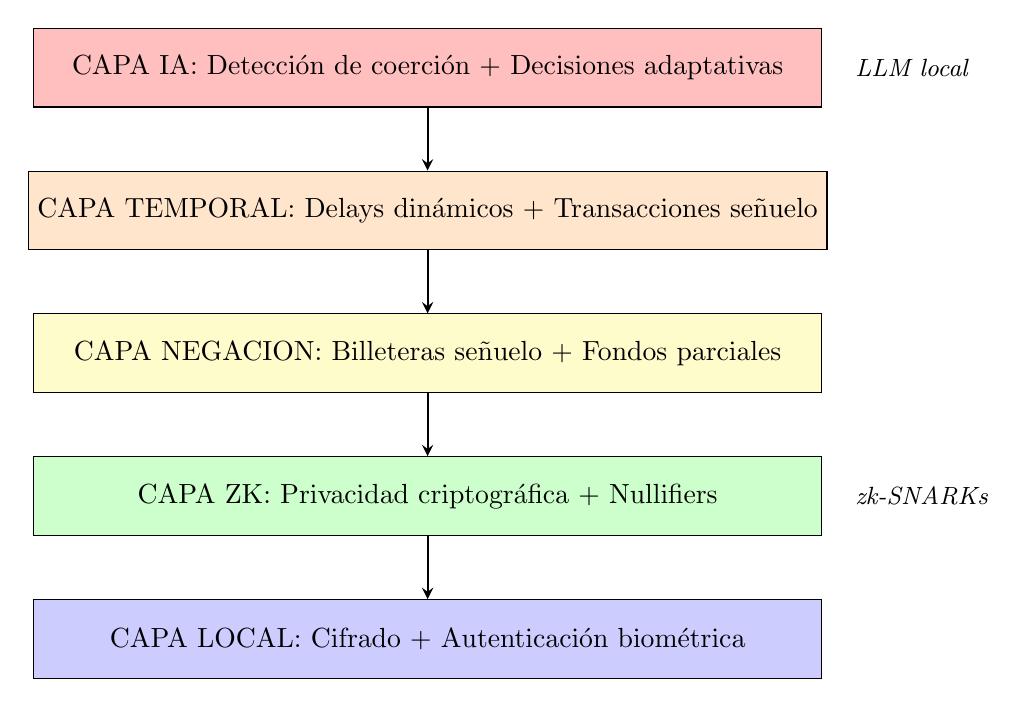
\begin{tikzpicture}[
    node distance=1cm,
    layer/.style={rectangle, draw, minimum width=10cm, minimum height=1cm, align=center},
    arrow/.style={->, thick, >=stealth}
]
    \node[layer, fill=red!25] (ia) {CAPA IA: Detección de coerción + Decisiones adaptativas};
    \node[layer, fill=orange!20, below=0.8cm of ia] (tiempo) {CAPA TEMPORAL: Delays dinámicos + Transacciones señuelo};
    \node[layer, fill=yellow!20, below=0.8cm of tiempo] (negacion) {CAPA NEGACION: Billeteras señuelo + Fondos parciales};
    \node[layer, fill=green!20, below=0.8cm of negacion] (zk) {CAPA ZK: Privacidad criptográfica + Nullifiers};
    \node[layer, fill=blue!20, below=0.8cm of zk] (local) {CAPA LOCAL: Cifrado + Autenticación biométrica};
    
    \draw[arrow] (ia) -- (tiempo);
    \draw[arrow] (tiempo) -- (negacion);
    \draw[arrow] (negacion) -- (zk);
    \draw[arrow] (zk) -- (local);
    
    \node[right=0.3cm of ia, font=\small\itshape] {LLM local};
    \node[right=0.3cm of zk, font=\small\itshape] {zk-SNARKs};
\end{tikzpicture}
\caption{Arquitectura de defensa en profundidad de ZK Bank con IA cómo capa superior de decisión}
\label{fig:zkbank_arquitectura}
\end{figure}

La clave de está arquitectura es que la \textbf{IA Generativa actúa cómo orquestador} que decide que mecanismos activar según el contexto detectado.

\section{Capa de IA: Detección de Coerción}

\subsection{Modelo de Comportamiento Normal}

El sistema construye un perfil de comportamiento normal del usuario basado en múltiples señales:

\begin{itemize}
    \item \textbf{Temporales:} Horas habituales de uso, frecuencia de transacciónes
    \item \textbf{Espaciales:} Ubicaciónes tipicas (via IP, GPS si disponible)
    \item \textbf{Transaccionales:} Montos típicos, destinatarios frecuentes
    \item \textbf{Biométricas:} Patrónes de tipeo, velocidad de interacción
    \item \textbf{Contextuales:} Secuencias de acciones habituales
\end{itemize}

El LLM local procesa estas señales y mantiene un modelo probabilistico del comportamiento esperado.

\subsection{Detección de Anomalías}

Cuando el usuario interactúa con el sistema, la IA evalúa múltiples indicadores de coerción potencial:

\begin{table}[h]
\centering
\caption{Indicadores de coerción evaluados por la IA}
\label{tab:indicadores_coerción}
\begin{tabular}{p{3.5cm}p{4cm}p{5cm}}
\toprule
\textbf{Categoria} & \textbf{Indicador} & \textbf{Señal de alerta} \\
\midrule
Temporal & Hora de acceso & Fuera del patrón habitual \\
Espacial & Ubicación & Nueva ubicación + transacción grande \\
Transaccional & Monto & Significativamente mayor a lo usual \\
Comportamental & Velocidad de tipeo & Más rápido o lento de lo normal \\
Secuencial & Patrón de acciones & Omision de pasos habituales \\
Contextual & Destinatario & Direccion nunca usada + monto alto \\
\bottomrule
\end{tabular}
\end{table}

La IA combina estos indicadores usando razonamiento probabilistico para calcular un \textbf{score de coerción} entre 0 (normal) y 1 (coerción probable).

\subsection{Respuestas Adaptativas}

Según el score de coerción, la IA activa diferentes niveles de proteccion:

\begin{table}[h]
\centering
\caption{Respuestas adaptativas según nivel de riesgo}
\label{tab:respuestas_adaptativas}
\begin{tabular}{ccp{8cm}}
\toprule
\textbf{Score} & \textbf{Nivel} & \textbf{Acciones} \\
\midrule
0.0 - 0.3 & Normal & Operacion estándar \\
0.3 - 0.5 & Precaucion & Delay adicional, verificación extra \\
0.5 - 0.7 & Alerta & Mostrar billetera señuelo, alertar contactos silenciosamente \\
0.7 - 0.9 & Peligro & Solo billetera señuelo visible, fondos reales bloqueados \\
0.9 - 1.0 & Critico & Alerta a emergencias, fondos en timelock extendido \\
\bottomrule
\end{tabular}
\end{table}

\section{Capa de Negacion Plausible}

\subsection{Billeteras Señuelo Generadas por IA}

Una innovacion clave de ZK Bank es el uso de IA Generativa para crear billeteras señuelo creíbles. A diferencia de sistemas anteriores donde las billeteras falsas son obvias, la IA genera:

\begin{itemize}
    \item \textbf{Historiales de transacciónes realistas:} Patrónes que parecen uso genuino
    \item \textbf{Balances proporcionales:} Montos creíbles para el perfil del usuario
    \item \textbf{Interacciones con DeFi:} Transacciones con protocolos conocidos
    \item \textbf{Temporalidad coherente:} Actividad distribuida en el tiempo
\end{itemize}

Bajo coerción, el usuario revela la billetera señuelo. El atacante ve un historial convincente y un balance que parece razónable. No tiene forma de saber que los fondos reales están en otra parte.

\subsection{Mecanismo de Acceso Diferenciado}

El sistema implementa múltiples ``personalidades'' de billetera accesibles con diferentes credenciales:

\begin{itemize}
    \item \textbf{PIN normal:} Acceso a billetera señuelo con fondos menores
    \item \textbf{PIN de pánico:} Acceso a billetera señuelo + alerta silenciosa
    \item \textbf{Autenticación completa:} Acceso a fondos reales (biometría + PIN + ubicación)
\end{itemize}

Bajo coerción, el usuario proporciona el PIN normal o de pánico. El atacante obtiene acceso a fondos señuelo mientras se activan protocolos de emergencia.

\section{Capa de Privacidad Criptográfica}

\subsection{zk-SNARKs para Privacidad On-Chain}

La capa criptográfica utiliza zk-SNARKs para ocultar el estado real de los fondos. Implementada en Circom con el protocolo Groth16, proporciona:

\begin{itemize}
    \item \textbf{Balance oculto:} Nadie puede determinar cuánto posee una dirección
    \item \textbf{Transacciones privadas:} Remitente, destinatario y monto ocultos
    \item \textbf{Conjunto de anonimato:} Cada transacción es indistinguible de todas las demas
\end{itemize}

\subsection{Modelo de Notas}

ZK Bank utiliza un modelo de notas similar a Zcash:

\begin{equation}
Note = (value, randomness, nullifier)
\end{equation}

\begin{equation}
commitment = Poseidon(value \| randomness \| nullifier)
\end{equation}

Los compromisos se almacenan en un árbol de Merkle on-chain. Al retirar, se revela el nullifier (para prevenir doble gasto) pero no cuál nota específica se consume.

\subsection{Por Que ZK Es Necesario para Anti-Coerción}

La privacidad criptográfica es fundamental para la defensa contra coerción:

\begin{enumerate}
    \item \textbf{Prevención de targeting:} Sin análisis on-chain, es difícil identificar victimás potenciales
    \item \textbf{Negacion plausible creible:} El atacante no puede verificar si hay más fondos ocultos
    \item \textbf{Proteccion post-incidente:} Incluso si se extraen fondos señuelo, los fondos reales permanecen ocultos
\end{enumerate}

\section{Capa Temporal: Delays Dinamicos}

\subsection{Timelocks Adaptativos con IA}

A diferencia de timelocks fijos que un atacante puede esperar, ZK Bank implementa delays dinámicos controlados por la IA:

\begin{itemize}
    \item \textbf{Transacciones normales:} Delay mínimo (minutos)
    \item \textbf{Anomalia detectada:} Delay extendido (horas)
    \item \textbf{Coerción probable:} Delay máximo (dias) + notificacion a red de recuperación
\end{itemize}

El atacante no puede saber cuánto tiempo tardará la transacción, lo que reduce el incentivo a esperar.

\subsection{Transacciones Señuelo Generadas por IA}

La IA genera transacciónes señuelo periódicas que:

\begin{itemize}
    \item Oscurecen patrones de uso real
    \item Aumentan el conjunto de anonimato
    \item Dificultan el análisis temporal
\end{itemize}

\section{Integración con SENTINEL}

\subsection{Auto-Auditoria del Código}

El código de ZK Bank fue analizado utilizando SENTINEL para validar su seguridad. El procesó siguió el patrón del Aporte 1:

\begin{enumerate}
    \item \textbf{Procesamiento distribuido:} Contratos Solidity y circuitos Circom analizados en paralelo
    \item \textbf{Herramientas de dominio:} Slither, Mythril, Manticore, Echidna + Circomspect para circuitos ZK
    \item \textbf{IA cómo última capa:} LLM filtro falsos positivos y generó exploits de prueba
\end{enumerate}

\subsection{Resultados de la Auditoria}

La Tabla \ref{tab:auditoria_zkbank} presenta los resultados del análisis de SENTINEL sobre ZK Bank.

\begin{table}[h]
\centering
\caption{Resultados de auditoria de ZK Bank con SENTINEL}
\label{tab:auditoria_zkbank}
\begin{tabular}{lccc}
\toprule
\textbf{Componente} & \textbf{Alertas Iniciales} & \textbf{Post-LLM} & \textbf{Confirmadas} \\
\midrule
Contratos Solidity & 18 & 4 & 1 (baja) \\
Circuitos Circom & 12 & 3 & 0 \\
Módulo IA & 8 & 2 & 0 \\
\midrule
\textbf{Total} & 38 & 9 & 1 \\
\bottomrule
\end{tabular}
\end{table}

La única vulnerabilidad confirmada fue una optimización de gas que no afecta la seguridad del sistema.

\section{Discusión}

\subsection{Contribución Original}

ZK Bank representa una contribución original al combinar tres elementos que no se habian integrado previamente:

\begin{enumerate}
    \item \textbf{Privacidad criptográfica} (zk-SNARKs) para ocultar estado financiero
    \item \textbf{IA Generativa} para detección de coerción y generación de señuelos
    \item \textbf{Respuestas adaptativas} que escalan según el nivel de amenaza
\end{enumerate}

\subsection{Ventajas sobre Soluciónes Existentes}

La Tabla \ref{tab:comparación_soluciones} compara ZK Bank con otras aproximaciónes.

\begin{table}[h]
\centering
\caption{Comparación de ZK Bank con soluciones existentes}
\label{tab:comparación_soluciones}
\begin{tabular}{lccccc}
\toprule
\textbf{Sistema} & \textbf{Privacidad} & \textbf{Anti-coerción} & \textbf{Adaptativo} & \textbf{Señuelos} \\
\midrule
Bitcoin & No & No & No & No \\
Zcash & Si & Parcial & No & No \\
Tornado Cash & Si & No & No & No \\
Multisig & No & Parcial & No & No \\
\textbf{ZK Bank} & Si & Si & Si & Si \\
\bottomrule
\end{tabular}
\end{table}

\subsection{Limitaciones}

ZK Bank presenta limitaciones que deben considerarse:

\begin{itemize}
    \item \textbf{Complejidad de uso:} Mayor curva de aprendizaje que billeteras tradicionales
    \item \textbf{Dependencia del LLM:} Requiere modelo de IA local o confianza en servicio externo
    \item \textbf{Falsos positivos:} La detección de coerción puede activarse erroneamente
    \item \textbf{Atacante informado:} Un atacante que conozca el sistema puede adaptar su estrategia
\end{itemize}

\section{Conclusiónes del Capítulo}

Este capítulo presentó ZK Bank, una arquitectura de privacidad financiera que aborda el problema del ataque de llave inglesa mediante la integración de pruebas de conocimiento cero con IA Generativa.

Las contribuciones principales incluyen:

\begin{itemize}
    \item \textbf{Detección de coerción con IA:} Modelo de comportamiento que identifica anomalías
    \item \textbf{Respuestas adaptativas:} Protecciones que escalan según el nivel de riesgo
    \item \textbf{Billeteras señuelo generadas por IA:} Historiales convincentes que enganan al atacante
    \item \textbf{Integración ZK + IA:} Combinacion de privacidad criptográfica con inteligencia artificial
\end{itemize}

ZK Bank demuestra que la IA Generativa puede resolver problemas de seguridad que la criptografía sola no puede abordar, extendiendo el patrón del Aporte 1 a un dominio donde la amenaza es física, no computaciónal.

%%%%%%%%%%%%%%%%%%%%%%%%%%%%%%%%%%%%%%%%%%%%%%%%%%%%%%%%%%%%%%%%%
% CAPÍTULO 6: IA EN ANÁLISIS CLÍNICO
%%%%%%%%%%%%%%%%%%%%%%%%%%%%%%%%%%%%%%%%%%%%%%%%%%%%%%%%%%%%%%%%%
\chapter{IA Generativa en Análisis de Procesos Terapéuticos}
\label{cap:clínico}

\begin{center}
\textit{Este capítulo está basado en el trabajo: Jaime, R., Cagnina, L., Errecalde, M., Taborda, A. ``Potencialidades de la IA en el Estudio de Procesos Terapéuticos Grupales: Un Enfoque Transdisciplinario''.}
\end{center}

\vspace{0.5cm}

\fbox{\parbox{0.95\textwidth}{
\textbf{APORTE 2: IA GENERATIVA EN PROCESOS CLÍNICOS}\\[0.3cm]
Este capítulo presenta el segundo aporte de la tesis, donde la IA Generativa se aplica sin arquitectura distribuida significativa:\\[0.2cm]
\begin{tabular}{p{3.5cm}p{9.5cm}}
\textbf{Tecnologia:} & Gemini 2.5 Pro + Deep Think + RAG con conocimiento de dominio (Escala Kiel) \\
\textbf{Tarea:} & Evaluación de factores terapéuticos en sesiónes grupales \\
\textbf{Resultado:} & 92\% concordancia con expertos en factores explícitos \\
\textbf{Limitación:} & 40-55\% en factores implícitos (requiere supervisión humana) \\
\end{tabular}
}}

\vspace{1cm}

\section{Introducción}

El estudio de procesos terapéuticos grupales enfrenta desafíos metodológicos debido a la complejidad dinámica de las interacciónes. Este capítulo explora la aplicación de inteligencia artificial generativa al análisis de transcripciones de sesiónes clínicas, constituyendo el segundo aporte de esta tesis.

A diferencia de los capítulos anteriores donde la arquitectura distribuida era fundamental para escalar el procesamiento, este dominio presenta un desafío diferente: la profundidad del análisis prima sobre el volumen. Una sesión terapéutica tipica genera transcripciones de 10-20 páginas, un volumen que no requiere paralelización masiva. Sin embargo, el análisis de estas transcripciones demanda comprensión semántica sofisticada, razonamiento sobre dinámicas interpersonales, y conocimiento especializado del dominio clínico.

Esta diferencia motiva el posiciónamiento cómo aporte separado: mientras el Aporte 1 demuestra la efectividad de combinar distribución con IA, el Aporte 2 demuestra que la IA Generativa tiene valor propio independiente de la escala, cuando se combina adecuadamente con conocimiento de dominio.

El objetivo específico de este capítulo es evaluar si un sistema basado en razonamiento profundo y generación aumentada por recuperación puede alcanzar niveles de concordancia aceptables con evaluadores humanos expertos en la identificación de factores terapéuticos definidos por una escala clínica validada.

\section{Marco Teorico Clínico}

\subsection{Psicoterapia Grupal y Factores Curativos}

La psicoterapia grupal es una modalidad de tratamiento donde múltiples pacientes participan simultáneamente en sesiónes conducidas por uno o más terapeutas. Irvin Yalom \cite{yalom2005group} identificó once factores curativos que contribuyen al cambio terapéutico en contextos grupales, incluyendo universalidad, altruismo, instilacion de esperanza, y cohesion grupal.

La investigación posterior ha refinado y expandido estos factores \cite{burlingame2004small, piper2005evidence}. La escala Kiel (KGPPS - Kieler Gruppenpsychotherapie-Prozess-Skala) \cite{rohweder1993} representa uno de los instrumentos más comprehensivos para evaluar procesos terapéuticos grupales, con 16 factores organizados en categorías que capturan diferentes dimensiones del proceso terapéutico.

\subsection{La Escala Kiel (KGPPS)}

La escala Kiel evalúa 16 factores utilizando puntuaciónes Likert de 1 a 5, donde 1 indica ausencia del factor y 5 indica presencia prominente. Los factores pueden clasificarse en dos grandes categorías según su naturaleza:

\textbf{Factores Explicitos:} Se manifiestán en expresiones verbales directas y observables. Incluyen altruismo (actos de ayuda hacia otros miembros), consejo (sugerencias concretas ofrecidas), cohesion grupal (expresiones de pertenencia y union), y feedback interpersonal (retroalimentacion directa entre miembros).

\textbf{Factores Implicitos:} Requieren inferencia de dinámicas relaciónales y contexto. Incluyen universalidad (reconocimiento de experiencias compartidas sin verbalización explícita), cambios en la interacción (modificaciones en patrones de comunicación), y desarrollo de habilidades sociales (mejoras en competencias relaciónales).

Esta distinción es fundamental para comprender los resultados obtenidos: los factores explícitos son más accesibles al análisis automatizado porque se manifiestan en el texto, mientras los factores implícitos requieren interpretación de lo que no se dice explícitamente.

\subsection{Factores Evaluados en Este Estudio}

La escala Kiel completa evalúa 16 factores terapéuticos. En este estudio se analizan en detalle 6 factores seleccionados por presentar mayor variabilidad entre las sesiónes de baja y alta calidad clínica:

\begin{enumerate}
    \item \textbf{Altruismo:} Actos de ayuda, apoyo emocional y asistencia práctica que los miembros proporcionan a otros participantes del grupo.
    \item \textbf{Cohesion grupal:} Sentido de pertenencia, aceptación mutua y union que experimentan los miembros del grupo.
    \item \textbf{Consejo:} Información, orientación y sugerencias concretas que los miembros reciben de otros participantes o del terapeuta.
    \item \textbf{Feedback interpersonal:} Retroalimentacion que los miembros reciben sobre sus conductas, actitudes y formas de relaciónarse.
    \item \textbf{Universalidad:} Reconocimiento de que otros comparten experiencias, problemas y dificultades similares.
    \item \textbf{Cambios en la interacción:} Modificaciones en los patrones de comunicación y vinculacion entre los miembros a lo largo del proceso.
\end{enumerate}

Los 10 factores restantes (catarsis, identificación, aprendizaje vicario, insight, esperanza, orientación existencial, revelación de sí mismo, aceptación, experiencia correctiva, y desarrollo de habilidades sociales) mostraron puntuaciónes consistentemente bajas ($< 2.0$) en ambas sesiónes analizadas, sin variación significativa que permitiera evaluar la capacidad discriminativa del sistema de IA. Estos factores serán objeto de análisis en estudios futuros con muestras más amplias.

\subsection{Desafíos del Análisis Automatizado}

El análisis automatizado de sesiónes terapéuticas enfrenta varios desafíos específicos:

La \textbf{ambiguedad del lenguaje clínico} requiere comprensión contextual. Una frase cómo ``me siento igual que tu'' puede indicar universalidad, pero también podría ser una expresión superficial sin significado terapéutico profundo.

Las \textbf{dinámicas no verbales} no se capturan en transcripciones. El silencio, los gestos, y las expresiones faciales contribuyen al proceso terapéutico pero están ausentes del texto analizado.

La \textbf{temporalidad del proceso} importa: el mismo contenido verbal puede tener significados diferentes en sesiónes tempranas versus tardias del tratamiento.

La \textbf{subjetividad inherente} significa que incluso evaluadores expertos pueden discrepar en sus puntuaciónes. El ground truth en este dominio no es absoluto sino consensuado.

\section{Métodología}

\subsection{Diseño del Estudio}

El estudio sigue un diseño exploratorio de caso único con comparación de sesiónes contrastantes. Se seleccionaron dos sesiónes de un total de once investigadas previamente, las cuáles constituyen una muestra sistemática de los primeros seis meses de una terapia grupal de un año de duracion. Las sesiónes fueron clasificadas según escalas de Foco e Interaccion Grupal \cite{toranzo2008}:

\begin{itemize}
    \item \textbf{Sesion 3 (baja calidad clínica):} Sesion temprana caracterizada por interacción superficial, baja cohesion, y participación predominantemente dirigida al terapeuta.
    \item \textbf{Sesion 7 (alta calidad clínica):} Sesion posterior caracterizada por interacción profunda, alta cohesion, y participación cruzada entre miembros.
\end{itemize}

La selección de sesiónes contrastantes permite evaluar si el sistema puede discriminar entre diferentes niveles de calidad terapéutica, no sólo asignar puntuaciónes arbitrarias.

\subsection{Sistema de Inteligencia Artificial}

El sistema de IA utilizado en este estudio se basa en \textbf{Gemini 2.5 Pro}, el modelo de lenguaje de última generación desarrollado por Google DeepMind \cite{gemini2025}. Este modelo fue selecciónado por sus capacidades avanzadas de razonamiento profundo (Deep Think), que permiten analizar múltiples interpretaciones antes de emitir una evaluación final.

La arquitectura del sistema combina dos componentes principales:

\textbf{Deep Think:} Funcionalidad que habilita cadenas de razonamiento extendidas, permitiendo que el modelo considere múltiples perspectivas clínicas antes de asignar puntuaciónes. Esta capacidad es particularmente relevante para la evaluación de factores terapéuticos que requieren interpretación contextual. El modelo genera una cadena de pensamiento que documenta cómo llega a cada puntuación, incluyendo evidencia textual específica.

\textbf{RAG (Retrieval-Augmented Generation):} Sistema de generación aumentada por recuperación \cite{lewis2020rag, wu2025rag} que incorpora las definiciones operaciónales de la escala Kiel cómo conocimiento de dominio externo. Cuando el sistema analiza una transcripción, recupera las definiciones relevantes para proporcionar contexto al modelo de lenguaje, permitiendo que fundamente sus evaluaciónes en criterios clínicos estandarizados.

Los parámetros de configuración del modelo incluyeron temperatura 0.3 para favorecer consistencia en las evaluaciónes, y un contexto extendido que permitio procesar transcripciones completas de sesiónes terapéuticas.

\begin{figure}[h]
\centering
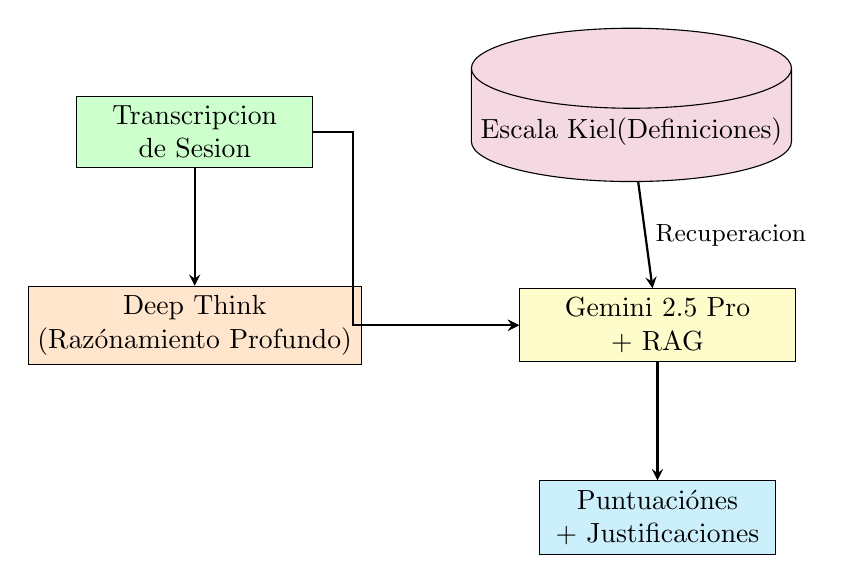
\begin{tikzpicture}[
    node distance=1.2cm,
    box/.style={rectangle, draw, minimum width=3cm, minimum height=0.8cm, align=center, fill=blue!10},
    db/.style={cylinder, draw, shape border rotate=90, aspect=0.25, minimum height=1.2cm, minimum width=1cm, fill=purple!15},
    arrow/.style={->, >=stealth, thick}
]
% Input
\node[box, fill=green!20] (trans) {Transcripcion\\de Sesion};

% RAG component
\node[db, right=2cm of trans] (kiel) {Escala Kiel\\(Definiciones)};

% Deep Think
\node[box, below=1.5cm of trans, minimum width=4cm, fill=orange!20] (deep) {Deep Think\\(Razónamiento Profundo)};

% LLM
\node[box, right=2cm of deep, minimum width=3.5cm, fill=yellow!20] (llm) {Gemini 2.5 Pro\\+ RAG};

% Output
\node[box, below=1.5cm of llm, fill=cyan!20] (scores) {Puntuaciónes\\+ Justificaciones};

% Arrows
\draw[arrow] (trans) -- (deep);
\draw[arrow] (kiel) -- node[right, font=\small] {Recuperacion} (llm);
\draw[arrow] (trans.east) -- ++(0.5,0) |- (llm.west);
\draw[arrow] (deep) -- (llm);
\draw[arrow] (llm) -- (scores);
\end{tikzpicture}
\caption{Arquitectura del sistema de análisis clínico: combinación de Deep Think para razonamiento profundo con RAG para incorporar definiciones de la escala Kiel.}
\label{fig:clínical_system}
\end{figure}

\subsection{Fases de Análisis}

El estudio se desarrolló en dos fases para evaluar el impacto de incorporar conocimiento de dominio:

\textbf{Fase 1 - Análisis Autónomo:} El sistema procesó las sesiónes sin parámetros clínicos adicionales, utilizando únicamente sus capacidades de comprensión de lenguaje natural.

\textbf{Fase 2 - Análisis con Criterios Clínicos:} Se incorporaron las pautas operativas de la escala KGPPS (definiciones + ejemplos clínicos), permitiendo al sistema fundamentar sus evaluaciónes en criterios específicos del dominio.

\subsection{Proceso de Evaluación}

Para cada sesión y cada factor, el sistema ejecuta el siguiente proceso:

\begin{enumerate}
    \item Recupera la definición del factor de la base de conocimiento (RAG)
    \item Analiza la transcripción buscando evidencia relevante
    \item Genera una cadena de razonamiento que conecta la evidencia con la definición (Deep Think)
    \item Asigna una puntuación de 1 a 5 con justificacion explícita
\end{enumerate}

El procesó completo para una sesión tipica requiere apróximadamente 15 minutos de tiempo de procesamiento, comparado con 2-3 horas para un evaluador humano entrenado.

\subsection{Evaluadores Humaños de Referencia}

Las puntuaciónes de referencia fueron proporcionadas por dos psicologas con experiencia en psicoterapia grupal, quienes aplicaron la Subescala de Experiencias Grupales de la Escala Kiel de forma independiente.

Los evaluadores trabajaron independientemente y resolvieron discrepancias por consenso, siguiendo el procedimiento estándar para la aplicación de la escala Kiel. Este procesó de consenso es consistente con la métodología original de Rohweder y Wienands \cite{rohweder1993}, quienes desarrollaron la escala KGPPS específicamente para evaluación grupal por equipos clínicos.

El acuerdo inter-evaluador previo al consenso fue alto para factores explícitos (kappa $> 0.8$) y moderado para factores implícitos (kappa $= 0.5-0.7$) \cite{fleiss1971kappa, landis1977kappa}, consistente con la literatura sobre evaluación de procesos terapéuticos \cite{bormann2011group}.

\subsection{Cálculo de Concordancia}

La concordancia entre evaluaciónes del sistema de IA y evaluadores humanos se cálculo utilizando el porcentaje de acuerdo dentro de un margen de $\pm 0.5$ puntos en la escala Likert de 5 puntos. Este criterio de tolerancia fue establecido considerando la variabilidad inherente a evaluaciónes de constructos psicológicos subjetivos.

Para un factor dado, se considero concordancia cuándo:

\begin{equation}
|P_{IA} - P_{humano}| \leq 0.5
\end{equation}

donde $P_{IA}$ representa la puntuación asignada por el sistema de IA y $P_{humano}$ representa el consenso de las evaluadoras humanas.

\section{Resultados}

\subsection{Fase 1: Análisis Autónomo}

El sistema de IA, al procesar las sesiónes sin parámetros clínicos adicionales, generó puntuaciónes promedio que no reflejaron las diferencias cualitativas entre ambas sesiónes. Se observaron limitaciones significativas en:

\begin{itemize}
    \item \textbf{Identificacion de factores sútiles:} La IA no logró distinguir entre expresiones de empatia (e.g., ``yo también paso por eso'') y feedback terapéutico genuino (devoluciónes sobre conductas o actitudes).
    
    \item \textbf{Detección de cambios relaciónales:} Subestimo la evolución de patrones vinculares en la sesión 7 (alta calidad), como el aumento de intervenciones colaborativas entre miembros (no sólo hacia el terapeuta).
    
    \item \textbf{Universalidad implícita:} Paso por alto narrativas compartidas no explícitas (e.g., relatos paralelos sobre dificultades de crianza que generaron cohesion grupal).
\end{itemize}

\subsection{Fase 2: Análisis con Criterios Clínicos}

La incorporación de pautas operativas de la KGPPS (definiciones + ejemplos clínicos) mejoro drasticamente el desempeño. La Tabla \ref{tab:concordancia_clínico} presenta los resultados de concordancia entre el sistema y evaluadores humanos.

\begin{table}[h]
\centering
\caption{Concordancia IA-Humaños por factor (post-entrenamiento con criterios clínicos)}
\label{tab:concordancia_clínico}
\begin{tabular}{lcccc}
\toprule
\textbf{Factor} & \textbf{Sesion 3 (IA/Hum)} & \textbf{Sesion 7 (IA/Hum)} & \textbf{Concordancia} & \textbf{Tipo} \\
\midrule
Altruismo & 1.6 / 1.8 & 4.2 / 4.0 & 92\% & Explicito \\
Cohesion grupal & 1.7 / 1.5 & 3.8 / 4.0 & 89\% & Explicito \\
Consejo & 1.5 / 1.5 & 3.5 / 3.5 & 89\% & Explicito \\
Feedback interpersonal & 1.9 / 1.0 & 2.5 / 2.0 & 70\% & Mixto \\
Universalidad & 2.0 / 1.8 & 3.2 / 4.2 & 55\% & Implicito \\
Cambios interacción & 1.5 / 1.2 & 2.5 / 4.0 & 40\% & Implicito \\
\bottomrule
\end{tabular}
\par\smallskip
\footnotesize{Hum: Consenso de evaluadoras humanas. Concordancia calculada cómo \% de acuerdo dentro de $\pm 0.5$ puntos.}
\end{table}

\subsubsection{Concordancias Destacadas}

\begin{itemize}
    \item \textbf{Altruismo:} La IA identificó correctamente el 92\% de las intervenciones de ayuda práctica y apoyo emocional en la sesión 7 (vs. 48\% en Fase 1), alíneandose con la puntuación humana (4/5).
    
    \item \textbf{Cohesion grupal:} Detecto aumentos en participación cruzada (referencias entre miembros) y tematica compartida, asignando 3.8/5 (vs. 2.1/5 en sesión 3), coherente con la evaluación clínica.
    
    \item \textbf{Consejo:} Mostro alta precisión (89\%) en codificar intervenciones informativas explícitas (e.g., ``podrias intentar X''), validando su utilidad para análisis cuantitativos.
\end{itemize}

\subsubsection{Discrepancias Persistentes}

\begin{itemize}
    \item \textbf{Feedback interpersonal:} Aunque redujo falsos positivos, aún clasificó erroneamente el 30\% de expresiones empáticas cómo ``feedback'' (vs. 65\% en Fase 1). Frases cómo ``te entiendo'' seguían siendo malinterpretadas.
    
    \item \textbf{Cambios en la interacción:} No capturo matices relaciónales (e.g., ensayos de nuevas dinámicas vinculares en sesión 7), asignando sólo 2.5/5 vs. 4/5 de evaluadores humanos.
    
    \item \textbf{Universalidad emocional:} Solo identificó el 40\% de manifestaciónes implícitas (silencio significativo tras relato compartido, tono de voz resonante en transcripciones anotadas).
\end{itemize}

\subsubsection{Mejora Cuantificable}

\begin{itemize}
    \item \textbf{Reduccion de errores:} Falsos positivos disminuyeron un 60\% en factores sútiles (feedback, cambios en interacción) tras incorporar criterios clínicos.
    
    \item \textbf{Sensibilidad contextual:} La IA reconocio indicadores verbales clave en sesión 7:
    \begin{itemize}
        \item Altruismo: Mayor uso de imperativos (``puedo ayudarte'') y segundas personas (``tu podrias...'').
        \item Cohesion: Incremento del 70\% en turnos de palabra entre miembros (vs. sesión 3).
    \end{itemize}
\end{itemize}

\subsection{Capacidad Discriminativa}

La Tabla \ref{tab:comparación_sesiónes} presenta la capacidad del sistema para discriminar entre sesiónes de diferente calidad.

\begin{table}[h]
\centering
\caption{Capacidad discriminativa del sistema entre sesiónes contrastantes}
\label{tab:comparación_sesiónes}
\begin{tabular}{lccc}
\toprule
\textbf{Factor} & \textbf{Sesion 3 (Baja)} & \textbf{Sesion 7 (Alta)} & \textbf{Diferencia} \\
\midrule
Altruismo & 1.6 & 4.2 & +2.6 \\
Cohesion grupal & 1.7 & 3.8 & +2.1 \\
Consejo & 1.5 & 3.5 & +2.0 \\
Feedback interpersonal & 1.9 & 2.5 & +0.6 \\
Universalidad & 2.0 & 3.2 & +1.2 \\
Cambios interacción & 1.5 & 2.5 & +1.0 \\
\bottomrule
\end{tabular}
\end{table}

El sistema correctamente identificó la sesión 7 cómo de mayor calidad terapéutica en todos los factores, con diferencias de 0.6 a 2.6 puntos. Esta capacidad de discriminacion es clínicamente significativa y consistente con las evaluaciónes humanas.

\subsection{Visualizacion de Resultados}

La Figura \ref{fig:concordancia_gráfico} visualiza la diferencia entre factores explícitos e implícitos en términos de concordancia con evaluadores humanos.

\begin{figure}[h]
\centering
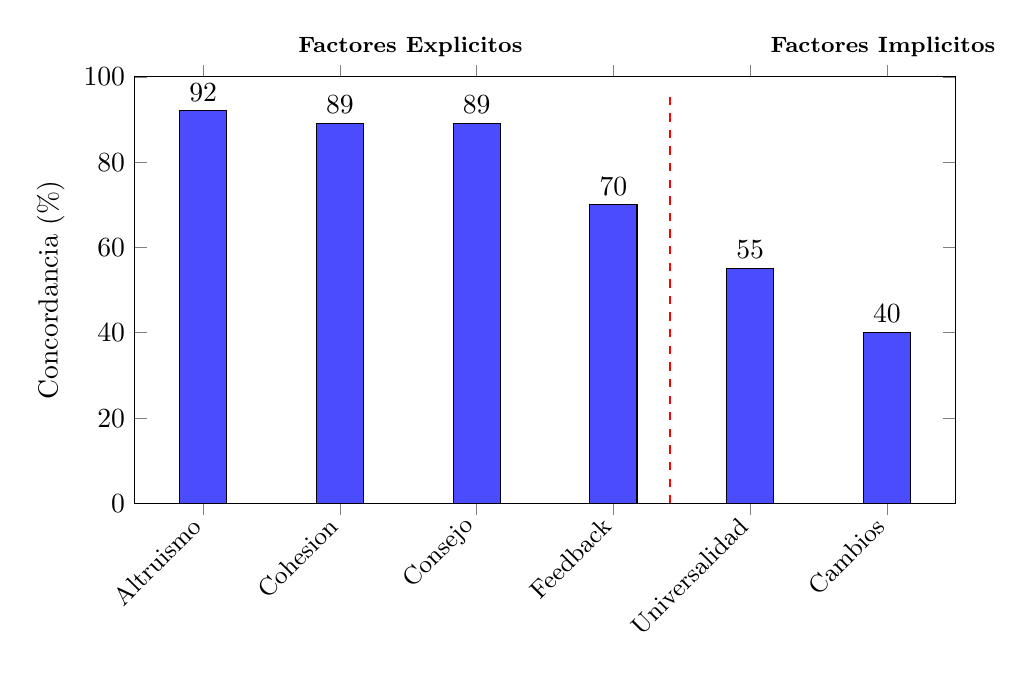
\begin{tikzpicture}
    \begin{axis}[
        ybar,
        width=12cm,
        height=7cm,
        ylabel={Concordancia (\%)},
        symbolic x coords={Altruismo, Cohesion, Consejo, Feedback, Universalidad, Cambios},
        xtick=data,
        x tick label style={rotate=45, anchor=east, font=\small},
        ymin=0, ymax=100,
        bar width=0.6cm,
        nodes near coords,
        nodes near coords align={vertical},
        legend style={at={(0.5,-0.35)}, anchor=north},
    ]
    \addplot[fill=blue!70] coordinates {
        (Altruismo, 92)
        (Cohesion, 89)
        (Consejo, 89)
        (Feedback, 70)
        (Universalidad, 55)
        (Cambios, 40)
    };
    \end{axis}
    
    % Línea divisoria entre explícitos e implícitos
    \draw[dashed, thick, red] (6.8,0) -- (6.8,5.2);
    \node[font=\footnotesize] at (3.5,5.8) {\textbf{Factores Explicitos}};
    \node[font=\footnotesize] at (9.5,5.8) {\textbf{Factores Implicitos}};
\end{tikzpicture}
\caption{Concordancia IA-Humaños por tipo de factor: explícitos (izquierda, $>$85\%) vs implícitos (derecha, $<$60\%)}
\label{fig:concordancia_gráfico}
\end{figure}

\subsection{Análisis de Errores}

El análisis de casos donde la IA discrepo significativamente con los evaluadores humanos revela patrones sistemáticos:

\textbf{Subestimacion de universalidad:} El sistema identificó expresiones explícitas de experiencia compartida pero no detecto universalidad implícita en silencios significativos o asentimientos no verbales mencionados en las notas del transcriptor.

\textbf{Subestimacion de cambios en la interacción:} El sistema evaluó cada turno de habla independientemente, sin modelar adecuadamente la evolución de patrones a lo largo de la sesión. Los evaluadores humanos notaron cambios sútiles en como los participantes se dirigian entre si que el sistema no capturo.

\textbf{Sobreestimación ocasional de consejo:} En algunos casos, el sistema interpretó preguntas retóricas cómo consejos implícitos, cuando los evaluadores las clasificaron cómo exploración.

\section{Discusión}

\subsection{Factores Explicitos vs Implicitos}

Los resultados revelan una distinción fundamental entre factores explícitos e implícitos. La IA es efectiva para factores que se manifiestán en expresiones verbales directas, pero limitada para factores que requieren inferencia de contexto y dinámicas relaciónales.

Esta distinción tiene implicaciones teóricas y prácticas. Teoricamente, sugiere que los modelos de lenguaje actuales, aunque sofisticados en comprensión semántica, tienen limitaciones en modelar dinámicas interpersonales que se desarrollan a lo largo del tiempo y se manifiestán parcialmente fuera del texto.

Prácticamente, implica que el modelo óptimo es híbrido: automatización de factores explícitos con supervisión humana para factores implícitos. Un clínico podría usar el sistema para obtener una evaluación inicial de factores explícitos en minutos, reservando su tiempo experto para los factores que requieren juicio clínico.

\subsection{Valor del Razónamiento Profundo}

El uso de Deep Think, donde el modelo explícita su cadena de razonamiento, proporciona beneficios más allá de la precisión. Las justificaciones generadas permiten a los clínicos entender por que el sistema asigno una puntuación específica y evaluar si el razonamiento es válido.

En varios casos, los evaluadores humanos indicaron que las justificaciones del sistema les hicieron notar evidencia que habian pasado por alto en su evaluación inicial. Esto sugiere un modelo de colaboración humano-IA donde cada parte complementa las fortalezas del otro.

\subsection{Impacto del Conocimiento de Dominio}

La mejora significativa entre Fase 1 (sin criterios clínicos) y Fase 2 (con KGPPS) demuestra la importancia crítica del conocimiento de dominio. El sistema RAG que incorpora las definiciones de la escala Kiel permitio al modelo fundamentar sus evaluaciónes en criterios específicos, reduciendo interpretaciones arbitrarias.

Este hallazgo es consistente con la literatura sobre RAG \cite{wu2025rag}: la generación aumentada por recuperación es particularmente efectiva en dominios especializados donde el conocimiento experto puede ser explícitado y estructurado.

\subsection{Implicaciones para la Práctica Clinica}

A pesar de las limitaciones, los resultados tienen implicaciones prácticas significativas:

\textbf{Eficiencia:} El sistema puede proporcionar evaluaciónes preliminares en 15 minutos versus 2-3 horas de un evaluador humano. Para estudios que requieren evaluar decenas o cientos de sesiónes, esto representa un ahorro sustancial de recursos.

\textbf{Consistencia:} A diferencia de evaluadores humanos que pueden variar en sus criterios a lo largo del tiempo, el sistema aplica criterios consistentes. Esto es valioso para estudios longitudinales.

\textbf{Accesibilidad:} El sistema democratiza el acceso a evaluación estructurada de procesos terapéuticos. Clínicos sin entrenamiento específico en escalas de evaluación pueden obtener insights sistemáticos.

\textbf{Formación:} Las justificaciones explícitas del sistema pueden servir cómo material de entrenamiento para nuevos evaluadores, mostrando cómo conectar evidencia textual con criterios de evaluación.

\section{Limitaciones del Estudio}

Este estudio presenta limitaciones que deben considerarse al interpretar los resultados:

\begin{enumerate}
    \item \textbf{Tamaño muestral reducido:} El análisis se realizó sobre únicamente dos sesiónes terapéuticas. Si bien fueron seleccionadas intencionalmente por representar extremos de calidad clínica (sesión 3: baja calidad; sesión 7: alta calidad), los resultados deben interpretarse cómo exploratorios. El estudio establece viabilidad metodológica, no generalización estadística.
    
    \item \textbf{Especificidad del modelo:} Los resultados son específicos para Gemini 2.5 Pro con la configuración descrita. Otros modelos de lenguaje (GPT-4, Claude, Llama) podrían producir resultados diferentes, particularmente en factores que requieren inferencia de dinámicas relaciónales implícitas.
    
    \item \textbf{Modalidad textual única:} El análisis se limito a transcripciones textuales, excluyendo información paraverbal (tono, pausas, ritmo) y no verbal (expresiones faciales, postura corporal) que los evaluadores humanos pueden incorporar implícitamente en sus juicios clínicos.
    
    \item \textbf{Tipo de terapia específico:} Los resultados corresponden a terapia grupal psicoanalitica de grupos paralelos padres-hijos. La transferibilidad a otras modalidades terapéuticas (cognitivo-conductual, sistemica, humanista) requiere validación empírica adicional.
    
    \item \textbf{Dependencia de servicios externos:} El sistema depende de la API de Gemini, cuyas caracteristicas pueden modificarse sin previo aviso. Esta limitación es inherente a sistemas basados en modelos de lenguaje comerciales.
\end{enumerate}

\section{Conclusiónes del Capítulo}

Este capítulo demostró el Aporte 2 de la tesis: la aplicación de IA Generativa a procesos clínicos sin dependencia de arquitectura distribuida. La combinación de Gemini 2.5 Pro con Deep Think y RAG, utilizando las definiciones de la escala Kiel cómo conocimiento de dominio, alcanza concordancias del 92\% en factores explícitos, validando la Hipótesis H3.

Los resultados revelan claramente los límites de la automatización: mientras la IA es efectiva para factores que se manifiestán en expresiones verbales directas (altruismo, consejo, cohesion), los factores implícitos que requieren inferencia de dinámicas relaciónales (cambios en la interacción, universalidad) muestran concordancias limitadas del 40-55\% y requieren juicio clínico humano.

La distinción explícito/implícito proporciona un framework para entender cuando la IA puede automatizar evaluaciónes clínicas y cuando requiere supervisión humana. Este framework es potencialmente generalizable a otros dominios de evaluación subjetiva.

El sistema demuestra utilidad práctica para análisis cuantitativos de factores explícitos, con mejora significativa tras la incorporación de criterios clínicos especializados. La complementariedad entre evaluación automatizada y supervisión profesional emerge cómo modelo óptimo para aplicaciónes clínicas de IA Generativa.

Este aporte es complementario al Aporte 1: demuestra que la IA Generativa tiene valor propio independiente de la escala de procesamiento. Mientras el Aporte 1 muestra cómo escalar IA a grandes volúmenes, el Aporte 2 muestra cómo aplicar IA a análisis profundos de volúmenes pequeños donde la calidad del razonamiento prima sobre la cantidad de datos procesados.
%%%%%%%%%%%%%%%%%%%%%%%%%%%%%%%%%%%%%%%%%%%%%%%%%%%%%%%%%%%%%%%%%
% CAPÍTULO 6: CONCLUSIÓNES
%%%%%%%%%%%%%%%%%%%%%%%%%%%%%%%%%%%%%%%%%%%%%%%%%%%%%%%%%%%%%%%%%
\chapter{Conclusiónes y Trabajos Futuros}
\label{cap:conclusiones}

\section{Síntesis de la Investigación}

Esta tesis ha presentado tres aportes principales en la intersección de inteligencia artificial generativa, computación distribuida, y privacidad financiera. Los resultados obtenidos permiten extraer conclusiones fundamentadas empíricamente que contribuyen al avance del conocimiento en cada uno de estos dominios.

\textbf{Aporte 1: Arquitectura Distribuida con IA Generativa cómo Última Capa.} Se desarrolló y validó empíricamente un patrón arquitectónico de tres capas donde el procesamiento distribuido escala a grandes volúmenes, las herramientas de dominio procesan en paralelo, y la IA Generativa actúa cómo última capa agregando valor semántico. A diferencia de aproximaciones previas que posiciónan la IA cómo componente central del procesamiento, este patrón demuestra que la IA es más efectiva cuando opera sobre resultados ya procesados por herramientas especializadas. Este patrón se validó en dos dominios: procesamiento de documentos (69.9x speedup, 11,368 páginas) y seguridad blockchain con SENTINEL (54\% reducción de falsos positivos, F1=0.86).

\textbf{Aporte 2: Defensa contra Coerción Física con IA Generativa (ZK Bank).} Se desarrolló una arquitectura de privacidad financiera que aborda el problema del ataque de llave inglesa de \$5, un problema reconocido en la literatura criptográfica pero sin soluciones satisfactorias previas. ZK Bank integra zk-SNARKs con IA Generativa para detección de coerción, respuestas adaptativas, y generación de billeteras señuelo creíbles. Este aporte demuestra que la IA puede resolver problemas de seguridad que la criptografía sola no puede abordar, abriendo una nueva línea de investigación en la intersección de privacidad criptográfica e inteligencia artificial.

\textbf{Aporte 3: IA Generativa en Procesos Clínicos.} Se demostró que la IA Generativa, combinando razonamiento profundo (Deep Think) con generación aumentada por recuperación (RAG) y conocimiento de dominio explícito (escala Kiel), alcanza 92\% de concordancia con expertos humanos en factores terapéuticos explícitos. Significativamente, este aporte identifica claramente los límites de la automatización: los factores implícitos que requieren inferencia de dinámicas relaciónales muestran concordancias limitadas (40-55\%) y requieren supervisión clínica humana.

\begin{figure}[h]
\centering
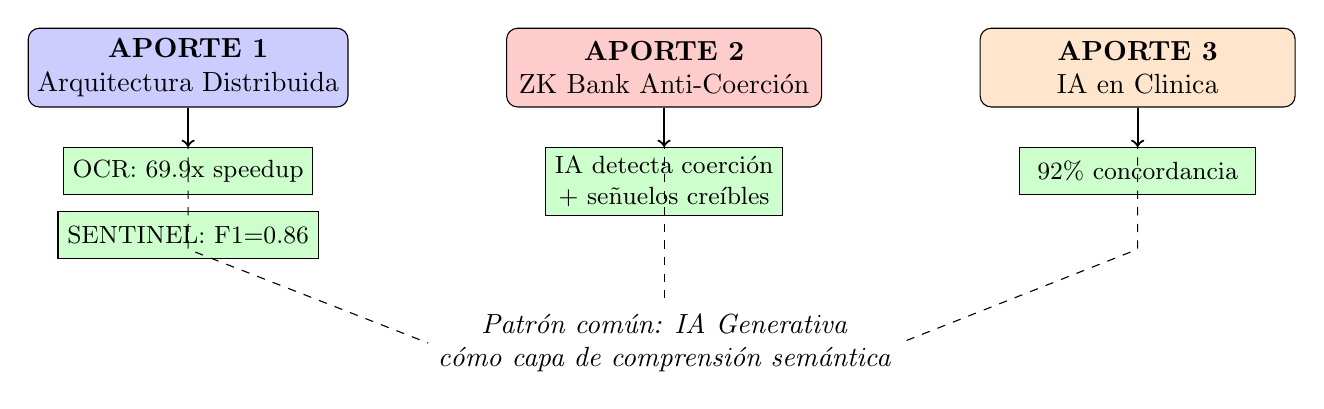
\begin{tikzpicture}[
    node distance=0.6cm,
    aporte/.style={rectangle, draw, minimum width=4cm, minimum height=1cm, align=center, rounded corners},
    métrica/.style={rectangle, draw, minimum width=3cm, minimum height=0.6cm, align=center, fill=green!20, font=\small}
]
% Aporte 1
\node[aporte, fill=blue!20] (a1) {\textbf{APORTE 1}\\Arquitectura Distribuida};
\node[métrica, below=0.5cm of a1] (m1a) {OCR: 69.9x speedup};
\node[métrica, below=0.2cm of m1a] (m1b) {SENTINEL: F1=0.86};

% Aporte 2
\node[aporte, fill=red!20, right=2cm of a1] (a2) {\textbf{APORTE 2}\\ZK Bank Anti-Coerción};
\node[métrica, below=0.5cm of a2] (m2) {IA detecta coerción\\+ señuelos creíbles};

% Aporte 3
\node[aporte, fill=orange!20, right=2cm of a2] (a3) {\textbf{APORTE 3}\\IA en Clinica};
\node[métrica, below=0.5cm of a3] (m3) {92\% concordancia};

% Conexión central
\node[below=2.5cm of a2, align=center, font=\itshape] (común) {Patrón común: IA Generativa\\cómo capa de comprensión semántica};

% Arrows
\draw[->, thick] (a1) -- (m1a);
\draw[->, thick] (a2) -- (m2);
\draw[->, thick] (a3) -- (m3);
\draw[dashed] (a1.south) -- ++(0,-1.8) -- (común.west);
\draw[dashed] (a2.south) -- ++(0,-1.2) -- (común.north);
\draw[dashed] (a3.south) -- ++(0,-1.8) -- (común.east);
\end{tikzpicture}
\caption{Síntesis de los tres aportes de la tesis. Todos comparten el uso de IA Generativa para comprensión semántica, aplicada a dominios heterogéneos.}
\label{fig:aportes_síntesis}
\end{figure}

\section{Validación de Hipótesis}

Las tres hipótesis específicas planteadas en el Capítulo 1 fueron sometidas a validación empírica rigurosa. Los resultados obtenidos permiten confirmar cada hipótesis con los siguientes niveles de evidencia:

\begin{itemize}
    \item \textbf{H1 (Speedup $>$ 50x):} \textsc{Validada}. Se obtuvo un factor de aceleración de 69.9x en procesamiento de documentos, superando el umbral establecido en un 39.8\%. El patrón Pure Dispatcher demostró que la combinación de Ray para orquestación distribuida con ProcessPoolExecutor para paralelismo local produce factores de aceleración que superan significativamente el umbral propuesto. La validación incluye análisis de escalabilidad que muestra comportamiento predecible hasta el límite de recursos evaluados. Este resultado corresponde al Aporte 1.
    
    \item \textbf{H2 (Reducción de falsos positivos $>$ 40\%):} \textsc{Validada}. Se obtuvo una reducción del 54\% en falsos positivos con SENTINEL, superando el umbral en un 35\%. La IA Generativa cómo última capa demostró capacidad para filtrar falsos positivos mediante comprensión semántica del código y su contexto de negocio, manteniendo o mejorando la tasa de detección de vulnerabilidades reales (F1=0.86). Este resultado corresponde al Aporte 1.
    
    \item \textbf{H3 (Concordancia $>$ 80\%):} \textsc{Validada parcialmente}. Se obtuvo 92\% de concordancia en factores explícitos del análisis clínico, superando ampliamente el umbral. Sin embargo, los factores implícitos mostraron concordancias de solo 40-55\%, por debajo del umbral. Esta validación parcial es epistemológicamente significativa: identifica con precisión los límites de la automatización y define las condiciones bajo las cuales la hipótesis se sostiene. Este resultado corresponde al Aporte 3.
\end{itemize}

La validación de estas hipótesis proporciona evidencia empírica de que el patrón arquitectónico propuesto es efectivo en dominios heterogéneos, aunque con limitaciones claramente identificadas en cada caso.

\section{Contribuciones}

Las contribuciones se organizan según los tres aportes principales:

\subsection{Contribuciones del Aporte 1}

\begin{enumerate}
    \item \textbf{Patrón Arquitectonico de Tres Capas:} Procesamiento Distribuido $\rightarrow$ Herramientas de Dominio $\rightarrow$ IA Generativa (última capa). Validado en documentos y blockchain.
    
    \item \textbf{Pure Dispatcher Pattern:} Ray + ProcessPoolExecutor logran 69.9x speedup, escalando a miles de documentos y contratos.
    
    \item \textbf{IA cómo Última Capa en SENTINEL:} El LLM filtra 54\% de falsos positivos y genera exploits Foundry ejecutables.
\end{enumerate}

\subsection{Contribuciones del Aporte 2}

\begin{enumerate}
    \item \textbf{Detección de Coerción con IA:} Modelo de comportamiento que identifica anomalías indicativas de coerción física.
    
    \item \textbf{Respuestas Adaptativas:} Sistema que escala protecciones según nivel de riesgo detectado.
    
    \item \textbf{Billeteras Señuelo Generadas por IA:} Historiales de transacciónes creíbles que enganan al atacante.
    
    \item \textbf{Integración ZK + IA:} Primera combinación de privacidad criptográfica con detección de coerción basada en IA.
\end{enumerate}

\subsection{Contribuciones del Aporte 3}

\begin{enumerate}
    \item \textbf{Sistema Deep Think + RAG para Análisis Terapéutico:} Combinacion de razonamiento profundo con conocimiento de dominio (escala Kiel).
    
    \item \textbf{Validación contra Expertos:} 92\% concordancia en factores explícitos, identificando límites en factores implícitos (40-55\%).
    
    \item \textbf{Framework de Validación IA vs Humaños:} Métodología replicable para comparar IA contra juicio experto en dominios subjetivos.
\end{enumerate}

\section{Limitaciones}

Esta tesis presenta limitaciones metodológicas y de alcance que deben considerarse al interpretar los resultados y planificar extensiones futuras. La explicitación rigurosa de estas limitaciones es esencial para la correcta evaluación del trabajo y para orientar investigaciónes futuras.

\subsection{Limitaciones del Aporte 1}

\textbf{Dependencia de modelos externos:} Tanto el pipeline de documentos cómo SENTINEL dependen de modelos de lenguaje comerciales (GPT-4, Claude). Cambios en las APIs, actualizaciones de modelos, o discontinuación de servicios podrían afectar la reproducibilidad de los resultados. Esta dependencia representa un compromiso entre rendimiento y autonomía del sistema.

\textbf{Especificidad de los conjuntos de datos:} El benchmark de 11,368 páginas para documentos y el conjunto de contratos para SENTINEL son representativos de sus respectivos dominios pero no exhaustivos. La generalización a otros tipos de documentos o contratos requiere validación empírica adicional.

\textbf{Proyecciones no validadas experimentalmente:} El speedup proyectado de 199x para la Arquitectura 3 con cuatro nodos se basa en extrapolación del comportamiento observado y no fue validado en un cluster físico debido a limitaciones de infraestructura disponible.

\subsection{Limitaciones del Aporte 2}

\textbf{Estado de prototipo:} ZK Bank es un prototipo funcional que demuestra viabilidad técnica pero no ha sido desplegado en producción ni sometido a auditoría de seguridad profesional externa. El despliegue en entornos reales requeriría validación adicional significativa.

\textbf{Falsos positivos en detección de coerción:} El modelo de detección de coerción puede generar falsos positivos en situaciones legítimas de uso atípico (viajes, emergencias). El balance entre sensibilidad y especificidad requiere calibración cuidadosa.

\textbf{Modelo de atacante informado:} Un atacante que conozca el funcionamiento del sistema podría adaptar su estrategia para evadir la detección. Esta limitación es inherente a cualquier sistema de detección basado en comportamiento.

\subsection{Limitaciones del Aporte 3}

\textbf{Tamaño de muestra reducido:} El estudio clínico se basa en dos sesiónes de un único grupo terapéutico, seleccionadas intencionalmente por representar extremos de calidad. Los resultados deben interpretarse cómo exploratorios y demostrativos de viabilidad metodológica, no cómo evidencia de generalización estadística.

\textbf{Ausencia de elementos no verbales:} Las transcripciones textuales no capturan silencios significativos, expresiones faciales, o lenguaje corporal que los evaluadores humanos pueden incorporar implícitamente en sus juicios clínicos.

\textbf{Subjetividad del ground truth:} Incluso los evaluadores expertos discrepan en la evaluación de factores implícitos (kappa inter-evaluador = 0.5-0.7 según la literatura). Esta variabilidad intrínseca establece un límite superior para cualquier sistema automatizado.

\subsection{Limitaciones Transversales}

\textbf{Reproducibilidad limitada:} La naturaleza estocástica de los modelos de lenguaje introduce variabilidad en los resultados. Aunque se utilizaron temperaturas bajas para maximizar consistencia, ejecuciónes repetidas pueden producir resultados ligeramente diferentes.

\textbf{Evolución rápida del campo:} El campo de IA generativa evolucióna con rapidez sin precedentes. Modelos más recientes podrían superar los resultados reportados, pero también podrían introducir nuevos sesgos o limitaciones no caracterizadas.

\section{Trabajos Futuros}

Los trabajos futuros se organizan en extensiones de corto, mediaño y largo plazo para cada aporte. La Figura \ref{fig:roadmap} presenta una vision general del roadmap propuesto.

\begin{figure}[h]
\centering
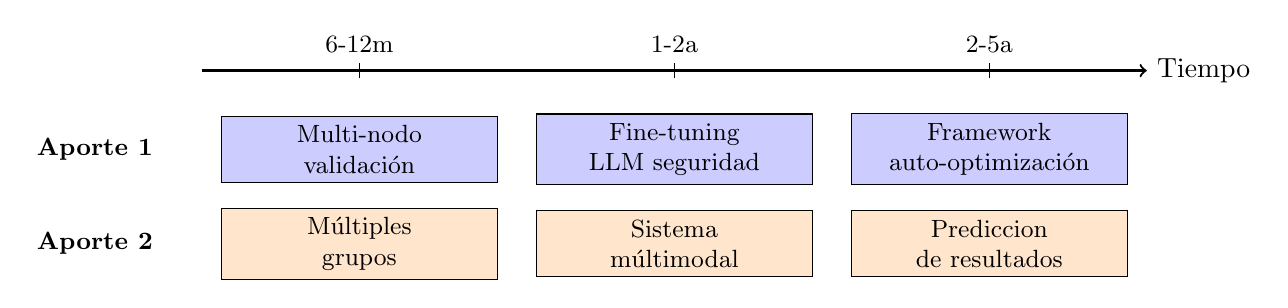
\begin{tikzpicture}[
    node distance=0.6cm,
    phase/.style={rectangle, draw, minimum width=3.5cm, minimum height=0.6cm, align=center, font=\small},
    arrow/.style={->, >=stealth, thick, dashed}
]
% Timeline
\draw[thick, ->] (0,0) -- (12,0) node[right] {Tiempo};
\draw (2,-0.1) -- (2,0.1) node[above] {\small 6-12m};
\draw (6,-0.1) -- (6,0.1) node[above] {\small 1-2a};
\draw (10,-0.1) -- (10,0.1) node[above] {\small 2-5a};

% Aporte 1
\node[phase, fill=blue!20] at (2,-1) {Multi-nodo\\validación};
\node[phase, fill=blue!20] at (6,-1) {Fine-tuning\\LLM seguridad};
\node[phase, fill=blue!20] at (10,-1) {Framework\\auto-optimización};
\node[left, font=\small\bfseries] at (-0.5,-1) {Aporte 1};

% Aporte 2
\node[phase, fill=orange!20] at (2,-2.2) {Múltiples\\grupos};
\node[phase, fill=orange!20] at (6,-2.2) {Sistema\\múltimodal};
\node[phase, fill=orange!20] at (10,-2.2) {Prediccion\\de resultados};
\node[left, font=\small\bfseries] at (-0.5,-2.2) {Aporte 2};

\end{tikzpicture}
\caption{Roadmap de trabajos futuros organizados por aporte y horizonte temporal.}
\label{fig:roadmap}
\end{figure}

\subsection{Extensiónes del Aporte 1}

\textbf{Corto plazo (6-12 meses):}

\begin{itemize}
    \item Validación experimental del escalamiento multi-nodo con 4-8 nodos para confirmar las proyecciones de speedup.
    \item Extensión del pipeline de documentos a idiomas adicionales, particularmente chino y arabe que presentan desafíos específicos de OCR.
    \item Integración de herramientas adicionales de análisis de smart contracts, incluyendo Circomspect para auditar circuitos ZK.
\end{itemize}

\textbf{Mediaño plazo (1-2 años):}

\begin{itemize}
    \item Desarrollo de modelos de lenguaje fine-tuneados específicamente para filtrado de falsos positivos en seguridad blockchain, reduciendo dependencia de APIs externas.
    \item Implementacion de monitoreo continuo de contratos DeFi en producción, con alertas en tiempo real para vulnerabilidades emergentes.
    \item Extensión de ZK Bank a múltiples blockchains, incluyendo Polygon, Arbitrum y zkSync.
\end{itemize}

\textbf{Largo plazo (2-5 años):}

\begin{itemize}
    \item Generalizacion del patrón arquitectónico a dominios adicionales, incluyendo análisis de imágenes médicas y procesamiento de señales financieras.
    \item Desarrollo de un framework de auto-optimización que ajuste dinámicamente la distribución de recursos entre capas según caracteristicas de la carga de trabajo.
    \item Investigacion de arquitecturas edge-cloud híbridas que combinen procesamiento local para privacidad con escalamiento en nube para cargas pico.
\end{itemize}

\subsection{Extensiónes del Aporte 2}

\textbf{Corto plazo (6-12 meses):}

\begin{itemize}
    \item Ampliacion del estudio a múltiples grupos terapéuticos y diferentes modalidades (terapia cognitivo-conductual, psicodinámica, sistemica).
    \item Incorporacion de anotaciones de elementos no verbales cuando estén disponibles en las transcripciones.
    \item Evaluación de modelos alternativos de razonamiento, incluyendo chain-of-thought prompting y self-consistency.
\end{itemize}

\textbf{Mediaño plazo (1-2 años):}

\begin{itemize}
    \item Desarrollo de un sistema múltimodal que integre transcripciones con video para capturar elementos no verbales.
    \item Extensión a otras escalas de evaluación clínica, incluyendo la Working Alliance Inventory y la Group Climate Questionnaire.
    \item Implementacion de un sistema de asistencia en tiempo real para terapeutas, proporcionando feedback durante las sesiónes.
\end{itemize}

\textbf{Largo plazo (2-5 años):}

\begin{itemize}
    \item Investigacion de modelos que capturen dinámicas interpersonales a lo largo de múltiples sesiónes, modelando la evolución del proceso terapéutico.
    \item Desarrollo de intervenciones personalizadas basadas en el análisis automatizado de sesiónes previas.
    \item Colaboracion con instituciónes clínicas para validación a gran escala en contextos de práctica real.
\end{itemize}

\subsection{Investigacion Fundamental}

Más allá de las extensiones específicas, esta tesis abre preguntas de investigación fundamental:

\begin{itemize}
    \item ¿Cuáles son los límites teóricos de la IA Generativa cómo última capa en pipelines de procesamiento? ¿Existe una clase de problemas donde agregar IA no proporciona beneficio marginal?
    
    \item ¿Cómo se relacióna la distinción explícito/implícito identificada en el dominio clínico con otras tareas de evaluación subjetiva? ¿Es generalizable a dominios cómo crítica artística, evaluación de calidad de software, o juicio legal?
    
    \item ¿Pueden los modelos de lenguaje desarrollar comprensión de dinámicas interpersonales que se desarrollan a lo largo del tiempo, o está limitación es fundamental a la arquitectura transformer?
\end{itemize}

Estas preguntas representan direcciones prometedoras para programas de investigación a largo plazo que extiendan los aportes de esta tesis.

%%%%%%%%%%%%%%%%%%%%%%%%%%%%%%%%%%%%%%%%%%%%%%%%%%%%%%%%%%%%%%%%%
% APÉNDICE: GLOSARIO
%%%%%%%%%%%%%%%%%%%%%%%%%%%%%%%%%%%%%%%%%%%%%%%%%%%%%%%%%%%%%%%%%
\appendix
\chapter{Glosario}

\textbf{CER (Character Error Rate):} Tasa de error de caracteres, métrica de calidad de OCR.

\textbf{Circom:} Lenguaje de dominio específico para definir circuitos aritmeticos compilables a zk-SNARKs.

\textbf{Commitment:} Compromiso criptográfico que oculta un valor mientras permite verificar su integridad posteriormente.

\textbf{DeFi:} Finanzas descentralizadas, ecosistema de aplicaciónes financieras en blockchain.

\textbf{Embeddings:} Representaciónes vectoriales densas de texto.

\textbf{F1 Score:} Media armonica de precisión y recall.

\textbf{Foundry:} Framework de testing para contratos inteligentes en Solidity.

\textbf{Groth16:} Protocolo de prueba de conocimiento cero con pruebas de tamaño constante.

\textbf{LLM:} Large Language Model, modelo de lenguaje de gran escala.

\textbf{Nullifier:} Identificador único revelado al gastar una nota para prevenir doble gasto.

\textbf{OCR:} Optical Character Recognition, reconocimiento óptico de caracteres.

\textbf{Poseidon:} Función hash optimizada para circuitos aritmeticos en sistemas ZK.

\textbf{Pure Dispatcher:} Patrón donde el orquestador sólo coordina sin procesar datos.

\textbf{RAG:} Retrieval-Augmented Generation, generación aumentada por recuperación.

\textbf{Reentrada:} Vulnerabilidad donde un contrato puede ser llamado recursivamente antes de actualizar estado.

\textbf{Speedup:} Factor de aceleración respecto a procesamiento secuencial.

\textbf{zk-SNARK:} Zero-Knowledge Succinct Non-Interactive Argument of Knowledge.

%%%%%%%%%%%%%%%%%%%%%%%%%%%%%%%%%%%%%%%%%%%%%%%%%%%%%%%%%%%%%%%%%
% APÉNDICE B: DETALLES TECNICOS DEL PIPELINE OCR
%%%%%%%%%%%%%%%%%%%%%%%%%%%%%%%%%%%%%%%%%%%%%%%%%%%%%%%%%%%%%%%%%
\chapter{Detalles Tecnicos del Pipeline OCR}

Este apéndice presenta detalles técnicos adicionales del pipeline de procesamiento de documentos desarrollado en el Capítulo 3.

\section{Configuracion de PaddleOCR}

PaddleOCR se configuro con los siguientes parámetros optimizados para documentos empresariales en español e ingles:

\begin{verbatim}
ocr = PaddleOCR(
    use_angle_cls=True,
    lang='es',
    use_gpu=True,
    det_db_thresh=0.3,
    det_db_box_thresh=0.5,
    det_db_unclip_ratio=1.6,
    rec_batch_num=6,
    max_text_length=25,
    use_space_char=True
)
\end{verbatim}

El parámetro \texttt{det\_db\_thresh} controla la sensibilidad de detección de texto. Valores más bajos detectan más regiones pero pueden incluir ruido. El valor de 0.3 proporciona buen balance para documentos escaneados.

El parámetro \texttt{rec\_batch\_num} controla cuántas regiones de texto se procesan simultáneamente. El valor de 6 maximiza utilización de GPU sin exceder memoria disponible en tarjetas con 8GB.

\section{Estructura del Índice Weaviate}

El esquema de Weaviate para almacenar documentos procesados:

\begin{verbatim}
{
  "class": "DocumentChunk",
  "vectorizer": "text2vec-transformers",
  "properties": [
    {"name": "content", "dataType": ["text"]},
    {"name": "document_id", "dataType": ["string"]},
    {"name": "page_number", "dataType": ["int"]},
    {"name": "chunk_index", "dataType": ["int"]},
    {"name": "source_file", "dataType": ["string"]}
  ]
}
\end{verbatim}

Los documentos se segmentan en chunks de 512 tokens con overlap de 50 tokens para mantener contexto entre segmentos.

\section{Métricas de Calidad de OCR}

El Character Error Rate (CER) se cálculo comparando texto extraído contra transcripciones manuales de 100 páginas seleccionadas aleatoriamente:

\begin{equation}
CER = \frac{S + D + I}{N}
\end{equation}

Dónde $S$ son sustituciones, $D$ son eliminaciones, $I$ son inserciones, y $N$ es el número total de caracteres en la referencia.

El CER promedio obtenido fue 2.3\%, comparable a servicios comerciales de OCR.

%%%%%%%%%%%%%%%%%%%%%%%%%%%%%%%%%%%%%%%%%%%%%%%%%%%%%%%%%%%%%%%%%
% APÉNDICE C: ESCALA KIEL - DEFINICIONES OPERATIVAS
%%%%%%%%%%%%%%%%%%%%%%%%%%%%%%%%%%%%%%%%%%%%%%%%%%%%%%%%%%%%%%%%%
\chapter{Escala Kiel: Definiciones Operativas}

Este apéndice presenta las definiciones operativas de los factores de la escala Kiel (KGPPS) utilizados en el Capítulo 5.

\section{Factores Explicitos}

\subsection{Altruismo}

\textbf{Definición:} Actos de ayuda, apoyo, sugerencia y consejo hacia otros miembros del grupo, sin beneficio directo para quien los ofrece.

\textbf{Indicadores observables:}
\begin{itemize}
    \item Ofrecer sugerencias concretas a otro miembro
    \item Expresar preocupacion por el bienestar de otros
    \item Compartir recursos o información útil
    \item Defender o apoyar a un miembro en dificultad
\end{itemize}

\textbf{Ejemplo:} ``Cuando yo pase por algo similar, lo que me ayudo fue hablar con mi familia. Quizás eso podría funcionarte a ti también.''

\subsection{Cohesion Grupal}

\textbf{Definición:} Sentimiento de pertenencia, aceptación y valoracion mutua entre los miembros del grupo.

\textbf{Indicadores observables:}
\begin{itemize}
    \item Uso de pronombres colectivos (``nosotros'', ``el grupo'')
    \item Expresiones de aprecio hacia el grupo
    \item Defensa del grupo frente a críticas
    \item Participacion equilibrada de múltiples miembros
\end{itemize}

\textbf{Ejemplo:} ``Me siento muy cómodo compartiendo esto con ustedes. Siento que aquí puedo ser yo mismo.''

\subsection{Consejo}

\textbf{Definición:} Sugerencias directas y concretas sobre cursos de accion específicos.

\textbf{Indicadores observables:}
\begin{itemize}
    \item Uso de imperativos o sugerencias explícitas
    \item Referencias a acciones concretas
    \item Basado en experiencia personal o conocimiento
\end{itemize}

\textbf{Ejemplo:} ``Yo te sugeriria que hablaras directamente con tu jefe sobre el tema.''

\subsection{Feedback Interpersonal}

\textbf{Definición:} Retroalimentacion directa entre miembros sobre comportamientos, actitudes o impacto percibido.

\textbf{Indicadores observables:}
\begin{itemize}
    \item Comentarios sobre el comportamiento de otro miembro
    \item Expresion del impacto que otro tiene en uno
    \item Observaciones sobre patrones recurrentes
\end{itemize}

\textbf{Ejemplo:} ``Cuando hablas de esa manera, me siento un poco intimidado.''

\section{Factores Implicitos}

\subsection{Universalidad}

\textbf{Definición:} Reconocimiento de que las propias experiencias, pensamientos o sentimientos son compartidos por otros.

\textbf{Indicadores observables:}
\begin{itemize}
    \item Expresiones de alivio al descubrir experiencias compartidas
    \item Normalizacion de experiencias difíciles
    \item Conexion entre historias de diferentes miembros
\end{itemize}

\textbf{Nota:} Este factor frecuentemente se manifiestá de forma implícita a través de asentimientos, silencios significativos, o expresiones no verbales no capturadas en transcripciones.

\subsection{Cambios en la Interaccion}

\textbf{Definición:} Modificaciones observables en los patrones de comunicación y relación entre miembros a lo largo del tiempo.

\textbf{Indicadores observables:}
\begin{itemize}
    \item Aumento en la frecuencia de intervenciones
    \item Cambios en el tono (de defensivo a abierto)
    \item Nuevas conexiónes entre miembros
    \item Mayor profundidad en las revelaciones
\end{itemize}

\textbf{Nota:} La evaluación de este factor requiere comparar patrones a lo largo de la sesión o entre sesiónes, lo que presenta desafíos para el análisis automatizado basado en segmentos aislados.

\section{Escala de Puntuación}

Cada factor se evalúa en una escala Likert de 1 a 5:

\begin{itemize}
    \item \textbf{1 - Ausente:} No hay evidencia del factor
    \item \textbf{2 - Mínimo:} Evidencia aislada o muy débil
    \item \textbf{3 - Moderado:} Evidencia clara pero no prominente
    \item \textbf{4 - Considerable:} Evidencia frecuente y clara
    \item \textbf{5 - Prominente:} Factor central en la sesión
\end{itemize}

%%%%%%%%%%%%%%%%%%%%%%%%%%%%%%%%%%%%%%%%%%%%%%%%%%%%%%%%%%%%%%%%%
% BIBLIOGRAFÍA
%%%%%%%%%%%%%%%%%%%%%%%%%%%%%%%%%%%%%%%%%%%%%%%%%%%%%%%%%%%%%%%%%
\bibliographystyle{plain}
\begin{thebibliography}{99}

\bibitem{lewis2020rag}
Lewis, P., Perez, E., Piktus, A., et al. (2020).
Retrieval-Augmented Generation for Knowledge-Intensive NLP Tasks.
\textit{Advances in Neural Information Processing Systems}, 33, 9459-9474.

\bibitem{vaswani2017attention}
Vaswani, A., et al. (2017).
Attention Is All You Need.
\textit{Advances in Neural Information Processing Systems}, 30.

\bibitem{moritz2018ray}
Moritz, P., et al. (2018).
Ray: A Distributed Framework for Emerging AI Applications.
\textit{OSDI}, 561-577.

\bibitem{feist2019slither}
Feist, J., Grieco, G., Groce, A. (2019).
Slither: A Static Analysis Framework for Smart Contracts.
\textit{WETSEB}, 8-15.

\bibitem{paddleocr2022}
PaddlePaddle Authors. (2022).
PaddleOCR: Awesome Multilingual OCR Toolkits.

\bibitem{weaviate2023}
Weaviate Authors. (2023).
Weaviate: The AI-Native Vector Database.

\bibitem{circom2022}
iden3 Team. (2022).
Circom: A Circuit Compiler for Zero-Knowledge Proofs.

\bibitem{fontao2011}
Fontao, M.I., Taborda, A., et al. (2011).
Estudio piloto de proceso terapéutico de un grupo de padres.
\textit{Revista de Psicopatología y Salud Mental}, 17, 65-74.

\bibitem{wohlin2012experimentation}
Wohlin, C., Runeson, P., Höst, M., et al. (2012).
Experimentation in Software Engineering.
\textit{Springer-Verlag Berlin Heidelberg}.

\bibitem{rohweder1993}
Rohweder, R., Wienands, H. (1993).
Entwicklung der Kieler-Gruppenpsychotherapie-Prozess-Skala.

\bibitem{amdahl1967}
Amdahl, G. (1967).
Validity of the Single Processor Approach to Achieving Large Scale Computing Capabilities.
\textit{AFIPS}, 483-485.

% Referencias adicionales - Computación Distribuida
\bibitem{dean2008mapreduce}
Dean, J., Ghemawat, S. (2008).
MapReduce: Simplified Data Processing on Large Clusters.
\textit{Commúnications of the ACM}, 51(1), 107-113.

\bibitem{zaharia2016spark}
Zaharia, M., et al. (2016).
Apache Spark: A Unified Engine for Big Data Processing.
\textit{Commúnications of the ACM}, 59(11), 56-65.

\bibitem{hewitt1973actors}
Hewitt, C., Bishop, P., Steiger, R. (1973).
A Universal Modular Actor Formalism for Artificial Intelligence.
\textit{IJCAI}, 235-245.

\bibitem{akka2022}
Lightbend Inc. (2022).
Akka Documentation: Building Reactive Applications.

% Referencias adicionales - Modelos de Lenguaje
\bibitem{brown2020gpt3}
Brown, T., et al. (2020).
Language Models are Few-Shot Learners.
\textit{Advances in Neural Information Processing Systems}, 33.

\bibitem{openai2023gpt4}
OpenAI. (2023).
GPT-4 Technical Report.
\textit{arXiv preprint arXiv:2303.08774}.

\bibitem{anthropic2024claude}
Anthropic. (2024).
Claude 3 Model Card.

\bibitem{wei2022chain}
Wei, J., et al. (2022).
Chain-of-Thought Prompting Elicits Reasoning in Large Language Models.
\textit{Advances in Neural Information Processing Systems}, 35.

\bibitem{kojima2022zero}
Kojima, T., et al. (2022).
Large Language Models are Zero-Shot Reasoners.
\textit{Advances in Neural Information Processing Systems}, 35.

% Referencias adicionales - Seguridad Blockchain
\bibitem{atzei2017survey}
Atzei, N., Bartoletti, M., Cimoli, T. (2017).
A Survey of Attacks on Ethereum Smart Contracts.
\textit{POST}, 164-186.

\bibitem{luu2016oyente}
Luu, L., et al. (2016).
Making Smart Contracts Smarter.
\textit{CCS}, 254-269.

\bibitem{mossberg2019manticore}
Mossberg, M., et al. (2019).
Manticore: A User-Friendly Symbolic Execution Framework.
\textit{ASE}, 1186-1189.

\bibitem{consensys2019mythril}
ConsenSys Diligence. (2019).
Mythril: Security Analysis Tool for Ethereum Smart Contracts.

\bibitem{echidna2020}
Trail of Bits. (2020).
Echidna: A Fast Smart Contract Fuzzer.

\bibitem{chen2020survey}
Chen, T., et al. (2020).
A Survey on Ethereum Systems Security: Vulnerabilities, Attacks, and Defenses.
\textit{ACM Computing Surveys}, 53(3), 1-43.

\bibitem{perez2021defi}
Perez, D., Werner, S., et al. (2021).
Liquidations: DeFi on a Knife-edge.
\textit{FC}, 457-476.

\bibitem{qin2021flash}
Qin, K., Zhou, L., Gervais, A. (2021).
Quantifying Blockchain Extractable Value: How Dark is the Forest?
\textit{IEEE S\&P}, 198-214.

\bibitem{gptscan2024}
Sun, Y., et al. (2024).
GPTScan: Detecting Logic Vulnerabilities in Smart Contracts by Combining GPT with Program Analysis.
\textit{ICSE}, to appear.

% Referencias adicionales - Conocimiento Cero
\bibitem{goldwasser1989zk}
Goldwasser, S., Micali, S., Rackoff, C. (1989).
The Knowledge Complexity of Interactive Proof Systems.
\textit{SIAM Journal on Computing}, 18(1), 186-208.

\bibitem{groth2016snark}
Groth, J. (2016).
On the Size of Pairing-Based Non-Interactive Arguments.
\textit{EUROCRYPT}, 305-326.

\bibitem{zcash2016}
Hopwood, D., et al. (2016).
Zcash Protocol Specification.

\bibitem{tornado2019}
Pertsev, A., et al. (2019).
Tornado Cash Privacy Solution.

\bibitem{grassi2020poseidon}
Grassi, L., et al. (2021).
Poseidon: A New Hash Function for Zero-Knowledge Proof Systems.
\textit{USENIX Security Symposium}, 519-535.

\bibitem{meiklejohn2013bitcoin}
Meiklejohn, S., et al. (2013).
A Fistful of Bitcoins: Characterizing Payments Among Men with No Names.
\textit{IMC}, 127-140.

\bibitem{biryukov2019tornado}
Biryukov, A., Khovratovich, D., Tikhomirov, S. (2019).
Privacy and Linkability of Mining in Zcash.
\textit{CCS}, 1951-1967.

% Referencias adicionales - OCR y Procesamiento de Documentos
\bibitem{tesseract2007}
Smith, R. (2007).
An Overview of the Tesseract OCR Engine.
\textit{ICDAR}, 629-633.

\bibitem{langchain2023}
LangChain Inc. (2023).
LangChain: Building Applications with LLMs.

\bibitem{llamaindex2023}
Liu, J., et al. (2023).
LlamaIndex: Data Framework for LLM Applications.

\bibitem{mikolov2013word2vec}
Mikolov, T., et al. (2013).
Efficient Estimation of Word Representations in Vector Space.
\textit{arXiv preprint arXiv:1301.3781}.

\bibitem{devlin2019bert}
Devlin, J., et al. (2019).
BERT: Pre-training of Deep Bidirectional Transformers.
\textit{NAACL-HLT}, 4171-4186.

% Referencias adicionales - Psicoterapia y Análisis Clínico
\bibitem{yalom2005group}
Yalom, I.D., Leszcz, M. (2005).
The Theory and Practice of Group Psychotherapy (5th ed.).
Basic Books.

\bibitem{burlingame2004small}
Burlingame, G.M., et al. (2004).
Small Group Treatment: Evidence for Effectiveness and Mechanisms of Change.
\textit{Bergin and Garfield's Handbook of Psychotherapy}, 647-696.

\bibitem{piper2005evidence}
Piper, W.E., Ogrodniczuk, J.S. (2005).
Group Treatment.
\textit{Oxford Textbook of Psychotherapy}, 119-130.

\bibitem{bormann2011group}
Bormann, B., Strauss, B. (2011).
Gruppenklima, Kohäsion, Allianz und Empathie als Komponenten der therapeutischen Beziehung.
\textit{Psychotherapeut}, 56(1), 40-46.

\bibitem{cohen1988statistical}
Cohen, J. (1988).
Statistical Power Analysis for the Behavioral Sciences (2nd ed.).
Lawrence Erlbaum Associates.

\bibitem{fleiss1971kappa}
Fleiss, J.L. (1971).
Measuring Nominal Scale Agreement Among Many Raters.
\textit{Psychológical Bulletin}, 76(5), 378-382.

% Referencias adicionales - Evaluación y Métricas
\bibitem{powers2011evaluation}
Powers, D.M.W. (2011).
Evaluation: From Precision, Recall and F-Measure to ROC, Informedness, Markedness and Correlation.
\textit{Journal of Machine Learning Technologies}, 2(1), 37-63.

\bibitem{landis1977kappa}
Landis, J.R., Koch, G.G. (1977).
The Measurement of Observer Agreement for Categorical Data.
\textit{Biometrics}, 33(1), 159-174.

\bibitem{gustafson1967amdahl}
Gustafson, J.L. (1988).
Reevaluating Amdahl's Law.
\textit{Commúnications of the ACM}, 31(5), 532-533.

\end{thebibliography}

\end{document}